\documentclass[11pt,a4paper]{article}

% ============================================================
% Packages
% ============================================================
\usepackage[utf8]{inputenc}
\usepackage[T1]{fontenc}
\usepackage{amsmath,amssymb,amsfonts}
\usepackage{graphicx}
\usepackage{booktabs}
\usepackage{multirow}
\usepackage{hyperref}
\usepackage{xcolor}
\usepackage{float}
\usepackage{enumitem}
\usepackage{algorithm}
\usepackage{algpseudocode}
\usepackage{natbib}
\usepackage[margin=1in]{geometry}
\usepackage{caption}
\usepackage{subcaption}
\usepackage{tabularx}
\usepackage{array}
\usepackage{tikz}
\usetikzlibrary{shapes.geometric, arrows.meta, positioning, calc, fit, backgrounds, decorations.pathreplacing}

\graphicspath{{paper_assets/}}

% TikZ styles
\tikzset{
    block/.style={rectangle, draw, fill=blue!12, text width=11em, text centered, rounded corners, minimum height=3em, font=\small},
    wideblock/.style={rectangle, draw, fill=blue!12, text width=14em, text centered, rounded corners, minimum height=3em, font=\small},
    phase/.style={rectangle, draw, fill=orange!22, text width=15em, text centered, rounded corners, minimum height=3em, font=\small\bfseries},
    data/.style={rectangle, draw, fill=green!15, text width=13em, text centered, rounded corners, minimum height=3em, font=\small},
    output/.style={rectangle, draw, fill=red!12, text width=12em, text centered, rounded corners, minimum height=3em, font=\small},
    persona/.style={rectangle, draw, fill=violet!15, text width=7em, text centered, rounded corners, minimum height=3.2em, font=\scriptsize},
    label/.style={font=\scriptsize\itshape, text=gray!70!black},
    arrow/.style={-{Stealth[length=2.5mm]}, thick},
}

\hypersetup{
    colorlinks=true,
    linkcolor=blue,
    citecolor=blue,
    urlcolor=blue
}

% ============================================================
\title{A New Generation of USD/INR Prediction Systems:\\
GDELT Sentiment, Variational Decomposition, Multi-Persona LLMs, Market Memory, and Topology-Enabled Predictions from Chaos}

\author{
    Dhruv Kumar\thanks{\texttt{dhruv.kumar@pilani.bits-pilani.ac.in}} \and
    Amrit Lahari\thanks{\texttt{f20230442@pilani.bits-pilani.ac.in}} \and
    Suyash Handa\thanks{\texttt{f20230029@pilani.bits-pilani.ac.in}} \and
    Shrey Bansal\thanks{\texttt{f20230649@pilani.bits-pilani.ac.in}}
}

\date{April 2026}

% ============================================================
\begin{document}

\maketitle

% ============================================================
% ABSTRACT
% ============================================================
\begin{abstract}
USD/INR forecasting is difficult because the Indian foreign exchange market is a managed-float system shaped by RBI intervention, imported energy shocks, dollar cycles, geopolitical events, and delayed rather than immediate news absorption. This paper consolidates the full research program embodied in the repository: Phase-A/Phase-B/Phase-C VMD and GDELT pipelines, EGARCH and hybrid volatility models, multi-model ensemble forecasting, regime-switching Monte Carlo simulation, the debiased Gemini V4 multi-persona architecture, the newer market-memory-first \texttt{final phase} stack, and the \texttt{TEPC} topology-chaos branch. Across the saved repo artifacts, raw aggregate signals are weak in isolation (Goldstein vs.\ IMF$_3$ correlation $= 0.010$; US average tone vs.\ USD/INR correlation $= 0.164$), but structured feature engineering recovers delayed signal: \texttt{Tone\_Economy} reaches a statistically significant correlation of $-0.147$ with IMF$_3$, meaningful-pattern analysis finds peak lags of 9 days for Goldstein and 12 days for tone, and the Phase-C danger-day classifier achieves 40\% precision with 52\% recall. In the historical Gemini track, V4 improves over V3 from 0.274\% to 0.270\% mean hybrid absolute error and from 61.3\% to 64.2\% directional accuracy under a sign-of-change evaluation, while January 2026 live predictions average 0.322\% absolute error. In the \texttt{final phase} walk-forward backtest, the memory-only ablation is strongest over 100 test days (MAE price 0.242, directional accuracy 61\%), indicating that compact shared state can outperform heavier feature blends. In the strict raw-GDELT TEPC run, \texttt{tepc\_full} leads on macro-F1 (0.337) with 77.5\% breakout accuracy, while persona blending reduces return MAE to 0.002695 and live 100-day runs show chaos features as the strongest classifier. The repository-wide conclusion is that USD/INR rewards regime detection, volatility classification, shared-state compression, and topology-aware modeling far more than naive direct price regression or heavyweight deep sequence models.
\end{abstract}

\textbf{Keywords:} USD/INR, GDELT, VMD, EGARCH, Monte Carlo, LLM Forecasting, Market Memory, TEPC, Chaos Modeling, Exchange Rate Prediction

% ============================================================
% 1. INTRODUCTION
% ============================================================
\section{Introduction}

Forecasting exchange rates remains one of the hardest problems in empirical finance. The central puzzle established by \citet{meese1983} still holds in modern settings: out-of-sample currency forecasting is notoriously brittle, and many structurally motivated models fail to beat simple benchmarks. This challenge is especially acute for USD/INR, where a managed-float regime, cross-asset dependence on oil and the dollar, event-driven sentiment shocks, and intermittent RBI intervention complicate the mapping from public information to next-day price movement. In such a market, a model can fit history extremely well while remaining economically useless in forward tests.

At the same time, the informational environment has changed. Global news databases such as GDELT provide dense coverage of political, economic, and geopolitical events in near real time \citep{leetaru2013}. Financial modeling has also broadened from classical volatility models \citep{bollerslev1986, nelson1991} toward boosted trees, neural sequence models, and more recently large language models (LLMs) and multi-agent reasoning systems \citep{chen2016xgboost, sezer2020, lopez2023, xie2023, li2024llm}. The repository studied in this paper is best understood as a research laboratory built around that shift: it starts from raw GDELT sentiment and macro data, progresses through VMD-based decomposition and danger-day classification, then evolves into LLM-assisted forecasting, memory-first hybrid modeling, and finally topology- and chaos-driven network forecasting.

This paper does not present a single homogeneous benchmark in which every model is evaluated under one frozen protocol. Instead, it documents and synthesizes the full research program captured by the repository. That distinction matters. The project contains multiple branches developed over time for different forecasting objectives: volatility classification, next-day point prediction, probabilistic scenario forecasting, walk-forward ablations under information embargo, and topology-aware breakout modeling. The scientific value lies in comparing these branches as complementary answers to the same core question: \textit{what kinds of signals and model structures actually survive contact with USD/INR?}

The central conclusion that emerges is pragmatic. USD/INR is not a market in which arbitrarily complex models automatically help. Raw aggregate sentiment is too weak; direct price regression is unstable; deep sequence models can fail spectacularly; and naive feature augmentation can worsen performance. Signal appears only after decomposition, thematic filtering, lag engineering, state compression, or network-level modeling. In other words, the market problem is not simply ``predict tomorrow's price'', but rather \textit{identify which layer of the market is predictable}: volatility, directional stress, shared market state, or synchronized macro-network regimes.

\subsection{Contributions}

Our main contributions are as follows:

\begin{itemize}[leftmargin=*]
    \item \textbf{Repository-wide synthesis of a multi-stage research program.} We consolidate the phase-based VMD/GDELT experiments, GARCH and ensemble branches, Gemini persona systems, the newer market-memory-first stack, and the TEPC topology-chaos branch into one coherent paper.

    \item \textbf{A transparent account of where signal actually appears in USD/INR.} We show that raw aggregate Goldstein signal is nearly useless on its own, while thematic filtering, lag analysis, and structured state representations recover delayed and economically interpretable predictive structure.

    \item \textbf{Evidence that off-the-shelf direct forecasting is poorly matched to this market.} ARIMA, SARIMA, GRU, LSTM, Attention, and several news-augmented regressors all underperform simple benchmarks or produce negative $R^2$, whereas volatility classification, market memory, and topology-aware models remain useful.

    \item \textbf{A detailed empirical bridge from LLM prompting to stateful and chaos-aware forecasting.} We document how the repository evolves from Gemini V4 debiased persona systems to the \texttt{final phase} memory-first framework and finally to TEPC, where graph topology and coupled Lorenz dynamics become first-class features.
\end{itemize}

\begin{figure*}[t]
\centering
\resizebox{\textwidth}{!}{%
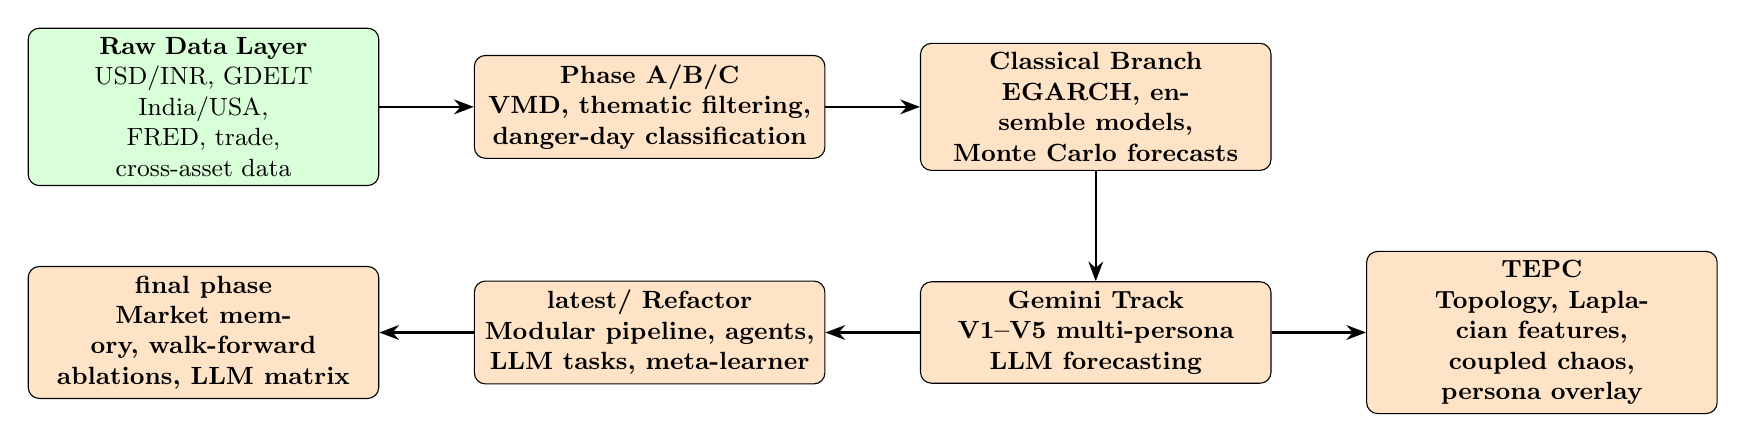
\begin{tikzpicture}[node distance=0.9cm]
    \node[data, text width=12em] (raw) {\textbf{Raw Data Layer}\\USD/INR, GDELT India/USA,\\FRED, trade, cross-asset data};

    \node[phase, right=1.2cm of raw, text width=12em] (phaseabc) {\textbf{Phase A/B/C}\\VMD, thematic filtering,\\danger-day classification};

    \node[phase, right=1.2cm of phaseabc, text width=12em] (classic) {\textbf{Classical Branch}\\EGARCH, ensemble models,\\Monte Carlo forecasts};

    \node[phase, below=1.4cm of classic, text width=12em] (gemini) {\textbf{Gemini Track}\\V1--V5 multi-persona\\LLM forecasting};

    \node[phase, left=1.2cm of gemini, text width=12em] (latest) {\textbf{latest/ Refactor}\\Modular pipeline, agents,\\LLM tasks, meta-learner};

    \node[phase, left=1.2cm of latest, text width=12em] (finalphase) {\textbf{final phase}\\Market memory, walk-forward\\ablations, LLM matrix};

    \node[phase, right=1.2cm of gemini, text width=12em] (tepc) {\textbf{TEPC}\\Topology, Laplacian features,\\coupled chaos, persona overlay};

    \draw[arrow] (raw) -- (phaseabc);
    \draw[arrow] (phaseabc) -- (classic);
    \draw[arrow] (classic) -- (gemini);
    \draw[arrow] (gemini) -- (latest);
    \draw[arrow] (latest) -- (finalphase);
    \draw[arrow] (gemini) -- (tepc);
\end{tikzpicture}}
\caption{Repository evolution as a research program rather than a single monolithic model. Early signal extraction work (Phase A/B/C) feeds the quantitative branches; Gemini V1--V5 introduces debiased multi-persona forecasting; \texttt{latest/} acts as a modular bridge; \texttt{final phase} formalizes market memory and walk-forward ablations; TEPC extends the program into dynamic topology and chaos-aware forecasting.}
\label{fig:evolution}
\end{figure*}

% ============================================================
% 2. RELATED WORK
% ============================================================
\section{Related Work}

\subsection{Exchange-Rate Forecasting and Volatility Modeling}

Exchange-rate predictability has long been constrained by the Meese--Rogoff result that structural models struggle to outperform naive random-walk baselines out of sample \citep{meese1983}. Later syntheses emphasized that no single specification consistently dominates across periods and regimes \citep{rossi2013, engel2014}. On the volatility side, GARCH-class models remain foundational because they explicitly model clustering and asymmetric shock transmission \citep{bollerslev1986, nelson1991}. Recent applied work has expanded into boosted trees and deep learning, but systematic reviews still report instability, overfitting, and sensitivity to sample regime and feature design \citep{chen2016xgboost, sezer2020}. Our repository-level findings align with this literature: classical volatility structure remains useful, but direct point forecasting is fragile.

\subsection{News Sentiment, GDELT, and Event-Derived Market Features}

Textual information has long been used as an alternative source of financial signal. Media pessimism can forecast subsequent price pressure \citep{tetlock2007}; large-scale collective mood measures can carry short-horizon market information \citep{bollen2011}; and text mining has become a recurring theme in financial prediction research \citep{nassirtoussi2014, wu2020sentiment}. GDELT is especially attractive because it exposes structured event metadata, Goldstein conflict-cooperation scores, tone values, and mention counts at global scale \citep{leetaru2013}. The gap addressed here is not access to news data per se, but the need to move beyond naive aggregation. The repository shows that raw aggregate scores are weak, while theme filtering, lag design, and event-intensity engineering create more useful features.

\subsection{LLMs, Multi-Agent Reasoning, and Finance}

LLMs have recently been studied as financial reasoners, sentiment extractors, and agent-like forecasters \citep{lopez2023, xie2023, wu2023bloomberggpt, li2024llm}. Prompt engineering and multi-agent decomposition are often used to diversify reasoning paths \citep{wei2022}. Yet the application of LLMs to numerical FX forecasting remains under-specified: the main risks are anchoring on recent price, prompt bias, narrative overconfidence, and lack of temporal learning. The repository addresses these issues in two ways. First, Gemini V4 introduces explicit debiasing via symmetric prompting, randomized direction order, and adaptive weighting. Second, the later \texttt{final phase} and TEPC systems reduce raw price exposure altogether by giving personas structured memory snapshots instead of unmediated spot-price context.

% ============================================================
% 3. REPOSITORY-WIDE RESEARCH DESIGN
% ============================================================
\section{Repository-Wide Research Design}

This paper is built from saved code, reports, plots, and output artifacts spanning the entire repository. Some branches are historical, others are current; some target volatility, others next-day price, and others breakout classification. Table~\ref{tab:repo_tracks} summarizes how these branches fit together.

\begin{table*}[t]
\centering
\small
\caption{Major research tracks represented in the repository.}
\label{tab:repo_tracks}
\resizebox{\textwidth}{!}{%
\begin{tabular}{p{2.2cm}p{3.2cm}p{4.8cm}p{4.8cm}}
\toprule
\textbf{Track} & \textbf{Core Files / Folders} & \textbf{Primary Research Question} & \textbf{Saved Artifacts Used Here} \\
\midrule
Phase A/B/C & \texttt{phase-a/}, \texttt{Phase-B/}, \texttt{Phase-C/} & Can decomposed and thematically filtered news signal identify IMF$_3$-style volatility and danger days? & \texttt{correlation\_results.csv}, \texttt{classifier\_performance.png}, \texttt{balanced\_confusion\_matrix.png}, lead-lag reports \\
GARCH branch & \texttt{GARCH/} & Does EGARCH plus engineered news/macro covariates improve return and volatility modeling? & \texttt{garch\_comparison.csv}, \texttt{feature\_importance.csv}, EGARCH plots \\
Ensemble / Monte Carlo & \texttt{ensemble\_model/}, \texttt{monte\_carlo\_simulation/} & Which quantitative family survives the USD/INR forecasting task, and what is the right uncertainty representation? & \texttt{ultimate\_model\_metrics.csv}, \texttt{ultimate\_weights.csv}, Monte Carlo statistics and fan-chart outputs \\
Gemini personas & \texttt{gemini\_preds/} & Can a debiased multi-persona LLM system improve short-horizon forecasts? & \texttt{simulation\_summary\_v3.csv}, \texttt{simulation\_summary\_v4.csv}, Jan 2026 live outputs \\
\texttt{latest/} & \texttt{latest/} & How should the older Gemini workflows be modularized into tasks, agents, cache, and meta-learning? & Treated here as an architectural bridge; the folder contains code but not a directly comparable saved plot suite \\
\texttt{final phase} & \texttt{final phase/} & Does a market-memory-first, walk-forward, embargoed hybrid system outperform raw feature stacks and persona-only baselines? & \texttt{ablation\_summary.csv}, \texttt{run\_summary.md}, multi-run comparison plots \\
TEPC & \texttt{TEPC/} & Does topology plus coupled chaos create a stronger breakout/return forecasting representation for INR/USD? & strict raw-GDELT and livepull run summaries, plot panels, persona overlay comparisons \\
\bottomrule
\end{tabular}}
\end{table*}

Two methodological cautions follow from this design. First, the paper reports \textit{branch-native} metrics rather than forcing all outputs onto an artificial unified leaderboard. Second, only reproducible artifacts present in the repository are reported numerically. The user request mentioned ARDL and DMI-style comparisons, but no versioned executable ARDL or DMI output files were present in the repository snapshot. We therefore report only implemented baselines rather than retrofitting undocumented numbers.

% ============================================================
% 4. DATA AND METHODOLOGY
% ============================================================
\section{Data and Methodology}

\subsection{Data Layers}

The repository integrates several data layers rather than a single flat table. At minimum these include daily USD/INR levels, India and USA GDELT event streams, FRED macro variables, bilateral Goldstein aggregates, thematic GDELT summaries, and later graph-structured TEPC node feeds. Table~\ref{tab:datasets} lists the most important datasets used across branches.

\begin{table*}[t]
\centering
\small
\caption{Core datasets used across the repository.}
\label{tab:datasets}
\resizebox{\textwidth}{!}{%
\begin{tabular}{lllll}
\toprule
\textbf{Dataset} & \textbf{Role} & \textbf{Rows / Records} & \textbf{Date Range} & \textbf{Notes} \\
\midrule
\texttt{india\_news\_gz\_combined\_sorted.csv} & Raw India GDELT news & 2,546,999 & 2025-01-01 to 2025-12-28 & Main India event archive used for thematic filtering and TEPC raw aggregation \\
\texttt{usa\_news\_combined\_sorted.csv} & Raw USA GDELT news & 14,377,323 & 2025-01-01 to 2025-12-30 & Cross-country comparison and TEPC raw USD-macro news nodes \\
\texttt{usd\_inr\_exchange\_rates\_1year.csv} & Daily FX level & 255 & 2024-12-30 to 2025-12-29 & One-year USD/INR series used by early scripts \\
\texttt{Phase-B/merged\_training\_data.csv} & Thematic + IMF$_3$ training frame & 254 & 2025-01-02 to 2025-12-26 & Central file for Phase-B/Phase-C/GARCH-style workflows \\
\texttt{combined\_goldstein\_exchange\_rates.csv} & Bilateral Goldstein layer & 253 & 2025-01-02 to 2025-12-29 & India/USA Goldstein summaries merged with USD/INR \\
\texttt{political\_news\_exchange\_merged.csv} & Political news aggregate layer & 252 & 2025-01-02 to 2025-12-24 & Event count, tone dispersion, Goldstein mean/std \\
\texttt{Super\_Master\_Dataset.csv} & Long-horizon macro master frame & 1,825 & 2019-01-02 to 2026-01-15 & Main multi-source dataset for later refactors and memory-based systems \\
\texttt{TEPC} live/strict feature frames & Graph-structured node panels & 214 strict rows; 321 livepull rows & strict: 2025-02-13 to 2025-12-24; livepull feature range: 2025-01-14 to 2026-04-10 & Derived inside TEPC runs rather than stored as one canonical root CSV \\
\bottomrule
\end{tabular}}
\end{table*}

\subsection{Phase A: Variational Mode Decomposition}

The first major methodological decision in the repository is to \textit{not} predict the raw USD/INR price with news. Instead, Phase A decomposes the exchange-rate signal into lower-frequency structure and high-frequency residual noise using Variational Mode Decomposition (VMD) \citep{dragomiretskiy2014}. The intuition is simple: macro fundamentals drive the long-run trend, while news is more likely to modulate the short-horizon residual.

Let $f(t)$ denote the exchange-rate series. VMD seeks modes $u_k(t)$ and center frequencies $\omega_k$ by minimizing the total bandwidth of the demodulated modes subject to reconstruction:
\begin{equation}
\min_{\{u_k\},\{\omega_k\}}
\sum_{k=1}^{K}
\left\|
\partial_t
\left[
\left(\delta(t) + \frac{j}{\pi t}\right) * u_k(t)
\right]
e^{-j\omega_k t}
\right\|_2^2
\quad \text{s.t.} \quad \sum_{k=1}^{K} u_k = f.
\end{equation}

The repository uses $K=3$ modes and targets IMF$_3$, the highest-frequency component, as the volatility/noise layer most likely to absorb daily news shocks. This decomposition step is one of the most important conceptual choices in the project: it reframes the problem away from exact long-run valuation and toward event-sensitive movement intensity.

\begin{figure}[t]
\centering
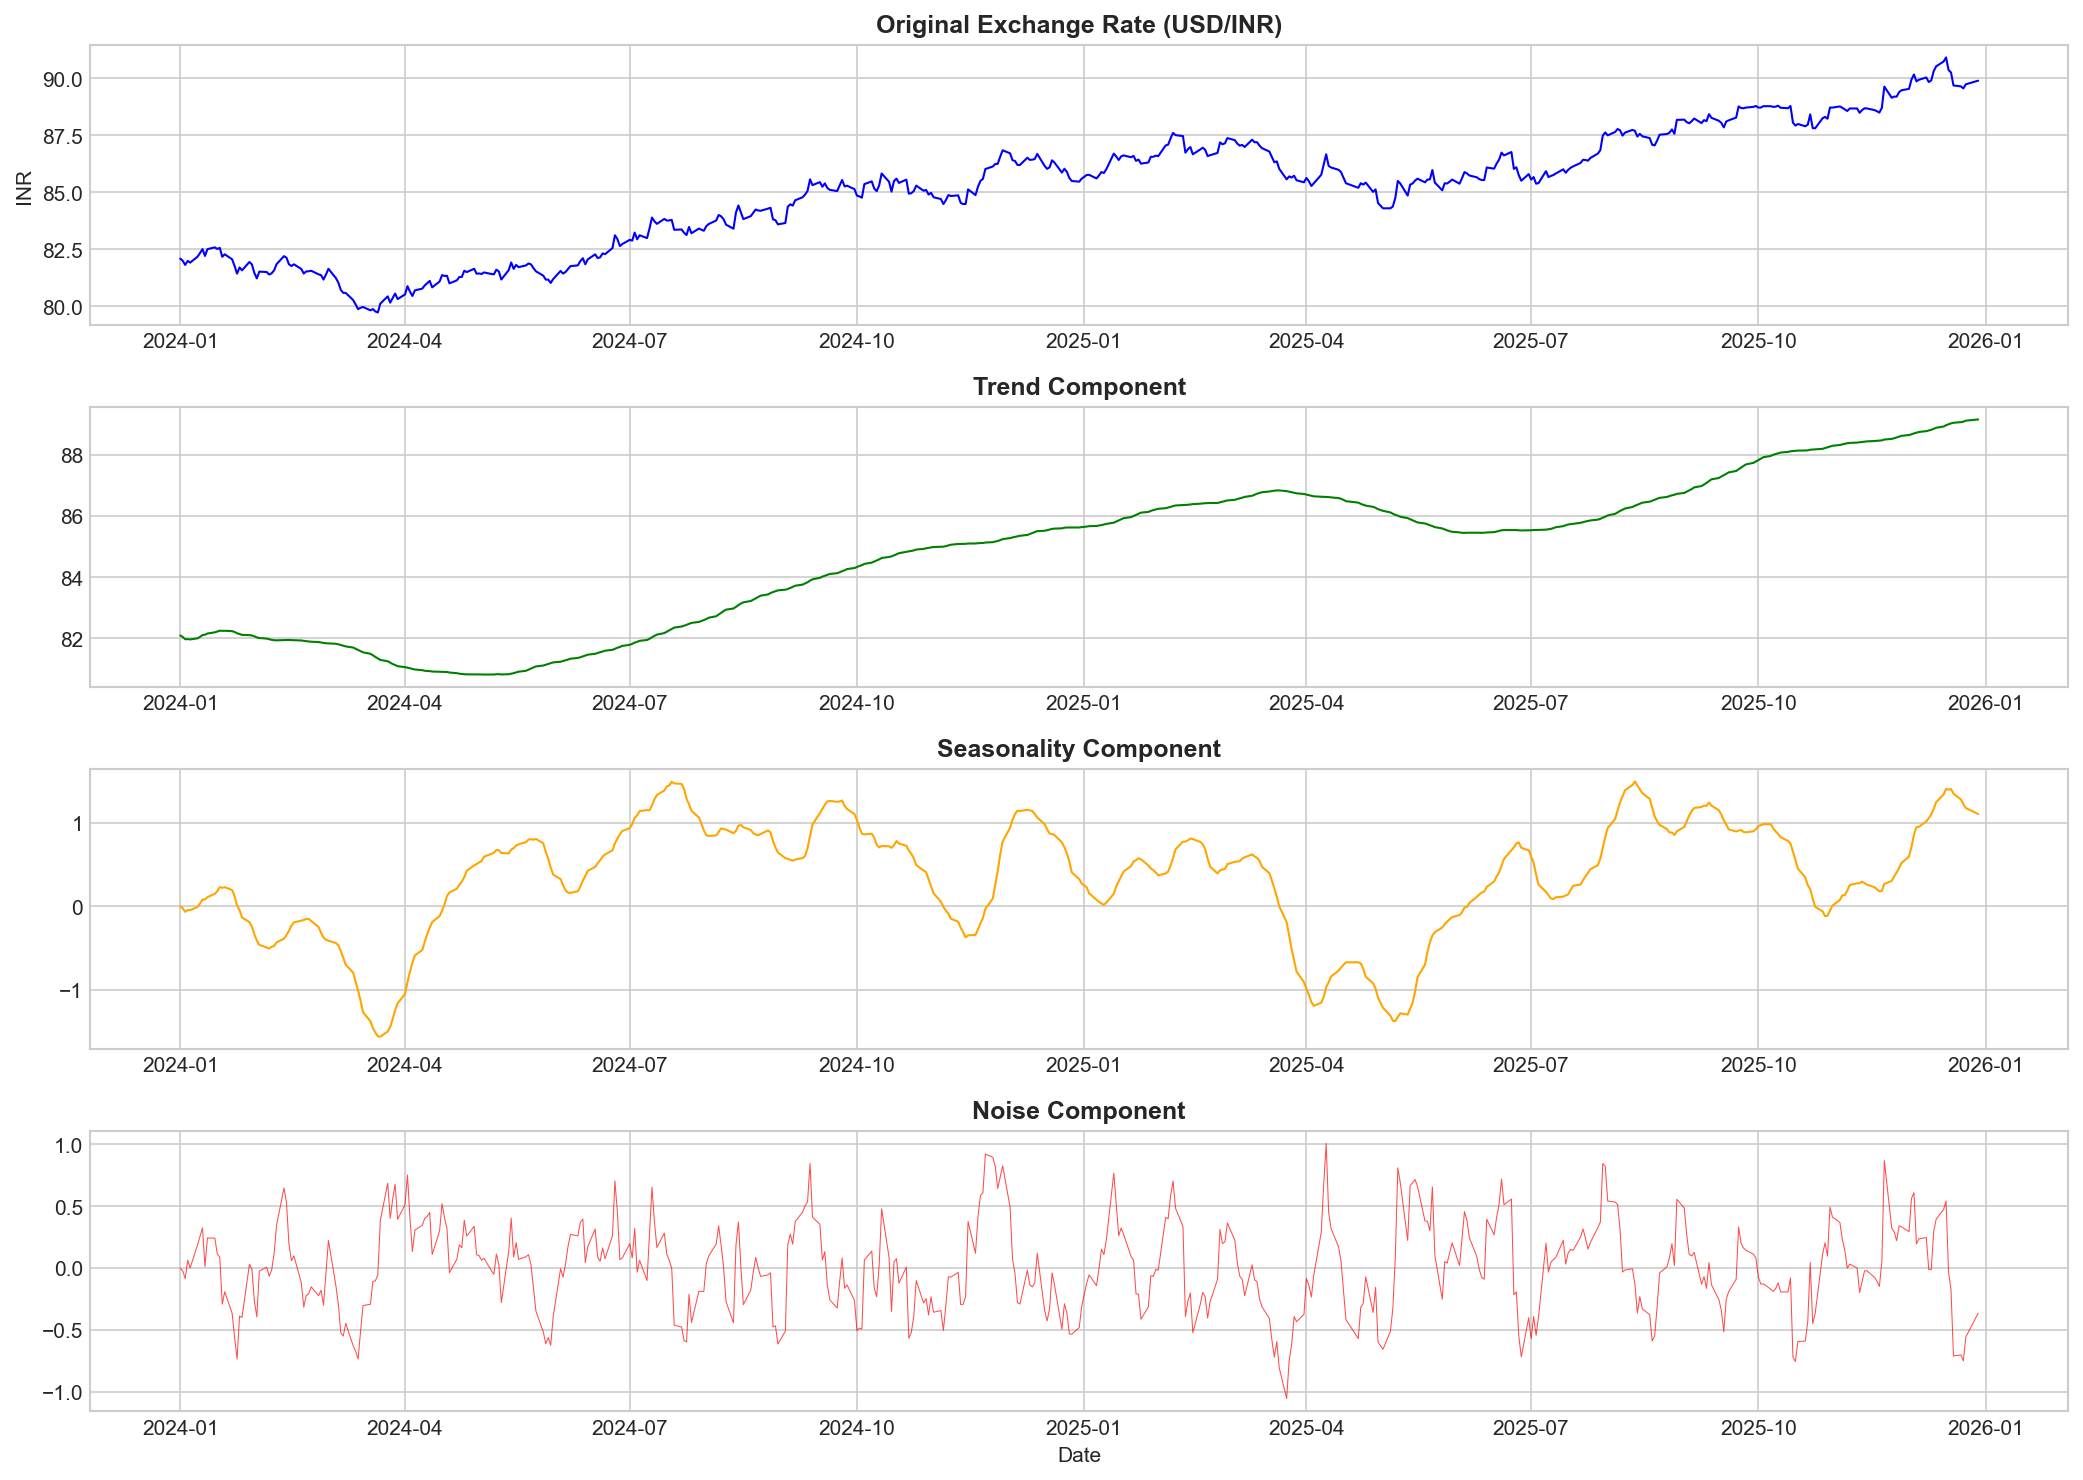
\includegraphics[width=\columnwidth]{ensemble_vmd_decomposition.png}
\caption{Representative VMD decomposition output saved by the ensemble branch. The decomposition separates the USD/INR series into trend, seasonal/cyclic, and noise-like components, with the high-frequency component treated as the most news-sensitive target in the early phases of the project.}
\label{fig:vmd}
\end{figure}

\subsection{Phase B: Thematic Filtering and Lag Engineering}

Naive sentiment aggregation proved too weak for this market. The repository therefore moves to domain-driven thematic filtering, grouping India-related GDELT articles into four currency-relevant themes:
\begin{enumerate}[leftmargin=*]
    \item \textbf{Economy} (139,953 articles): RBI policy, inflation, GDP, forex, reserves, trade, taxation.
    \item \textbf{Conflict} (560,938 articles): protests, crisis, border tension, attacks, strikes, military events.
    \item \textbf{Policy} (594,924 articles): cabinet actions, legislation, ministerial and parliamentary policy events.
    \item \textbf{Corporate} (53,779 articles): major Indian corporates, mergers, scandals, acquisitions, firm-specific shocks.
\end{enumerate}

From these themes the repository constructs 16 daily features spanning tone, Goldstein, counts, and spike variables. A key engineered feature is the impact-weighted Goldstein score:
\begin{equation}
\text{Goldstein}_{\text{weighted}} = \sum_i \text{GoldsteinScale}_i \times \text{NumMentions}_i,
\end{equation}
which distinguishes between a low-attention event and a widely propagated market shock. Later branches extend the same logic into rolling averages, signed log transforms, event heat, and shared memory pressure variables.

\begin{figure*}[t]
\centering
\begin{subfigure}[t]{0.58\textwidth}
    \centering
    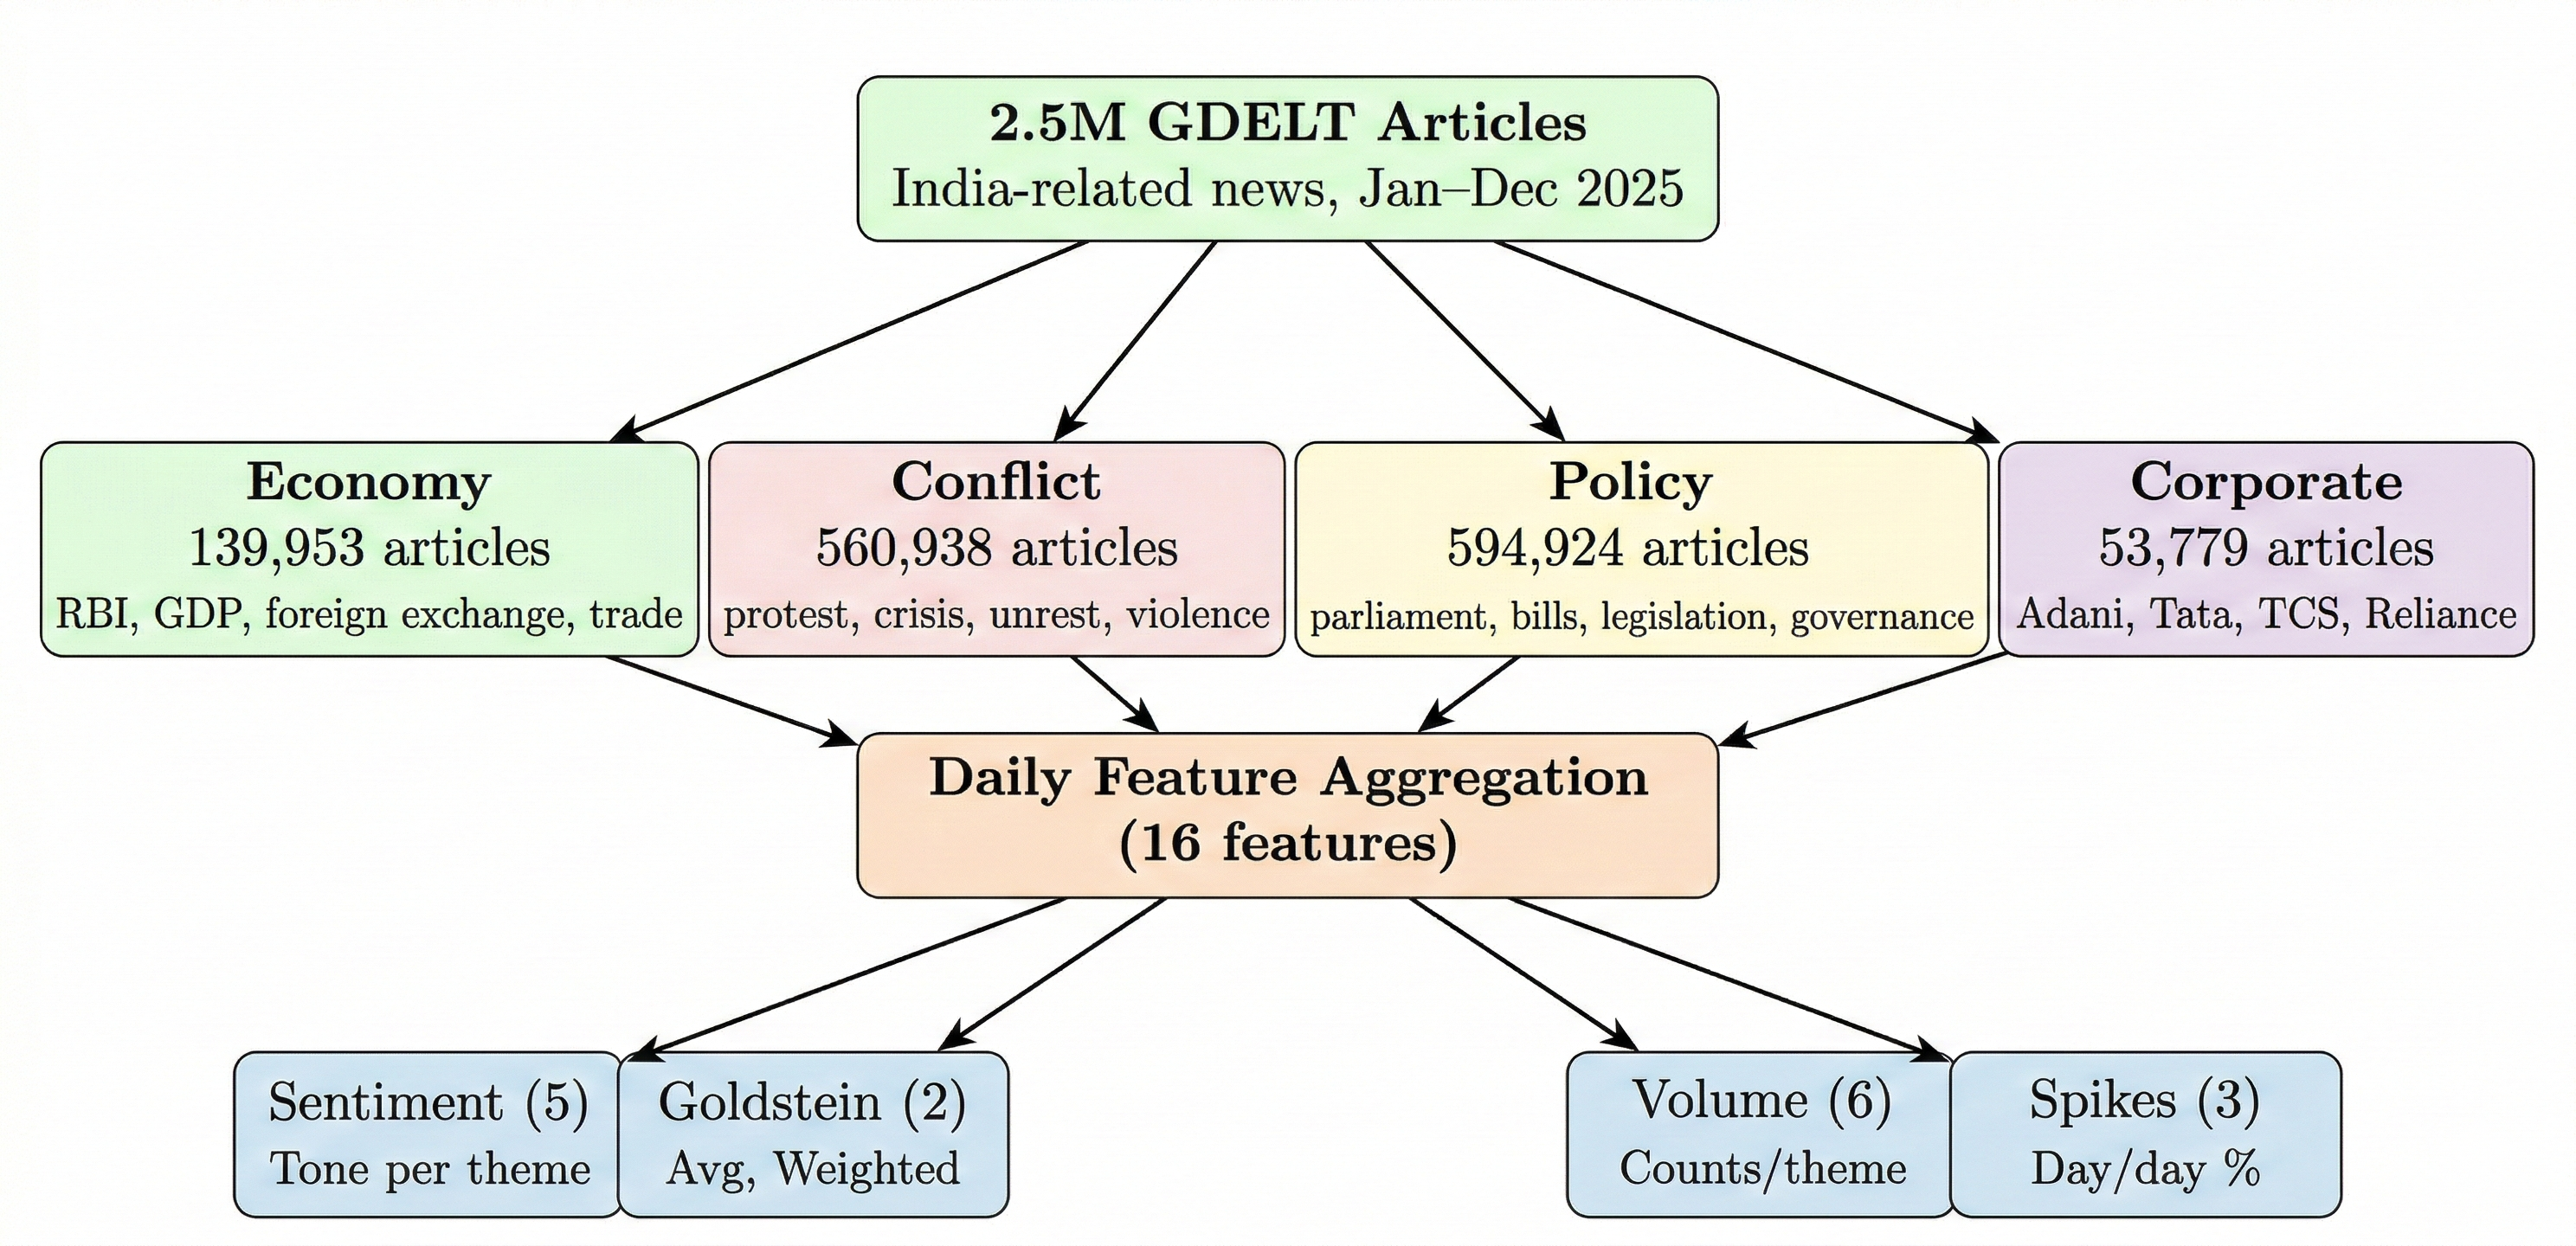
\includegraphics[width=\linewidth]{phase_b_theme_pipeline.png}
    \caption{Theme-filtering and aggregation pipeline used to turn raw GDELT into daily features.}
\end{subfigure}
\hfill
\begin{subfigure}[t]{0.38\textwidth}
    \centering
    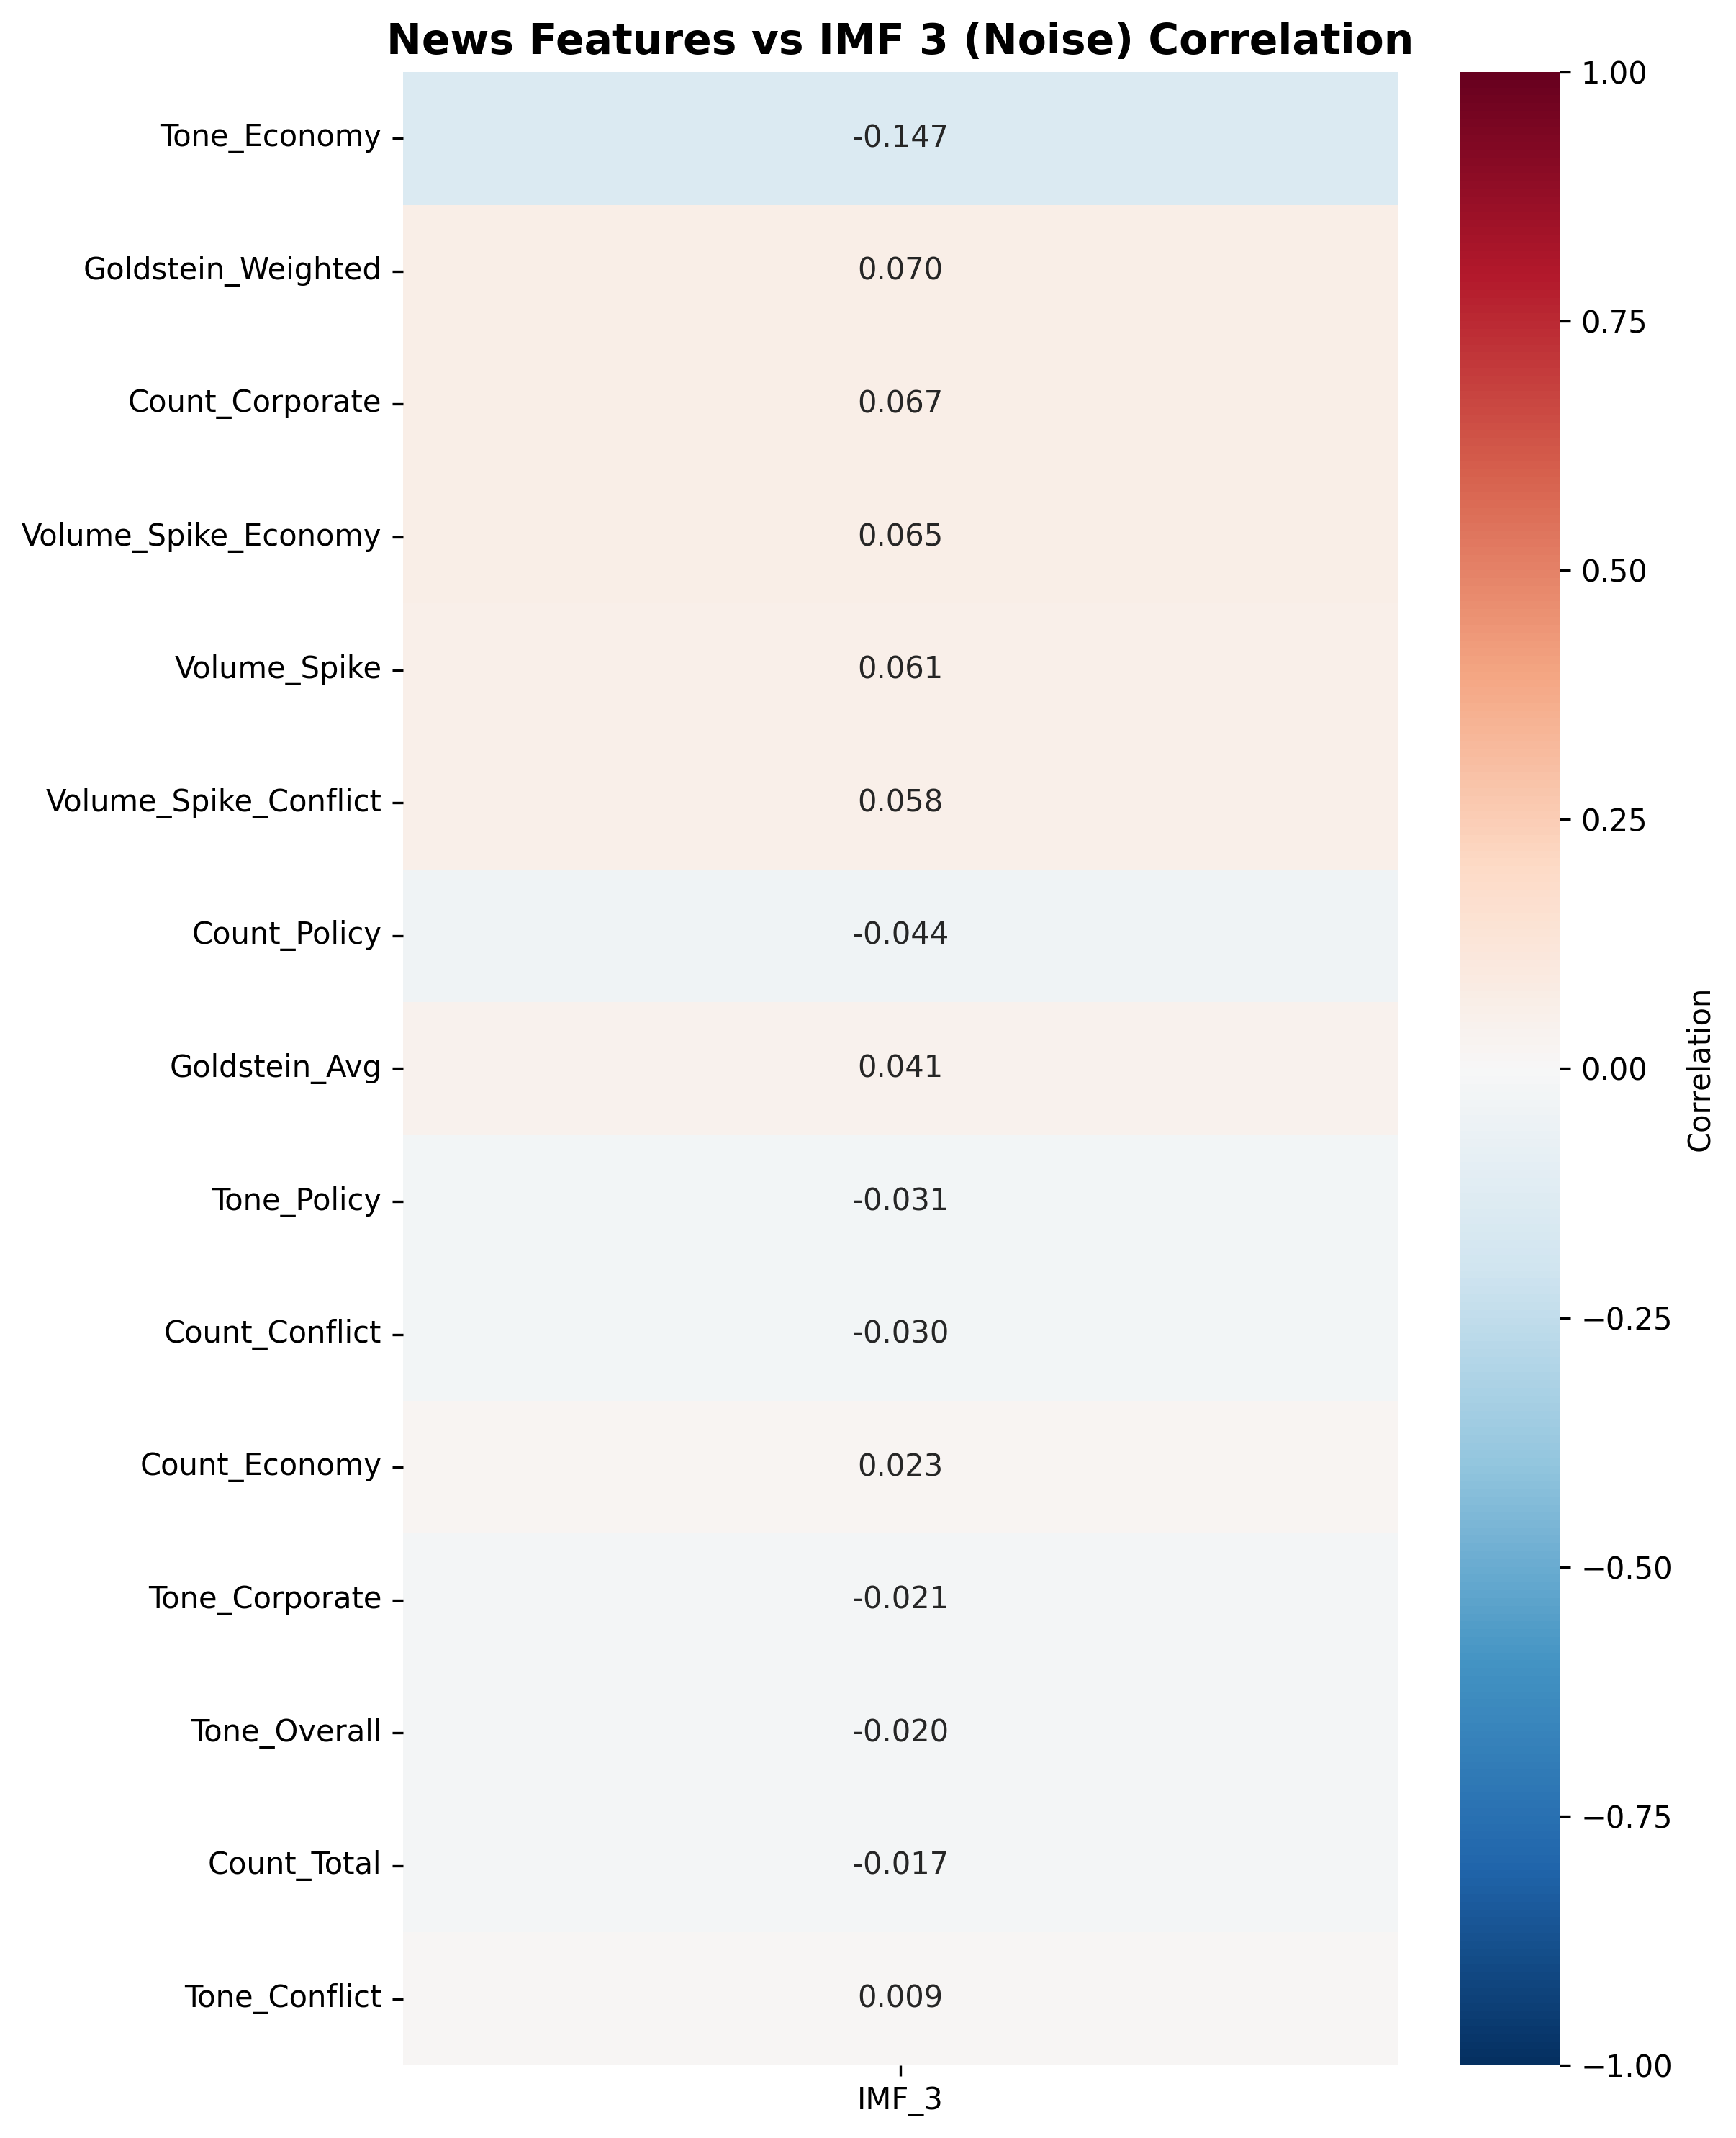
\includegraphics[width=\linewidth]{phase_b_heatmap.png}
    \caption{Correlation heatmap from the Phase-B outputs.}
\end{subfigure}
\caption{Phase-B transforms raw GDELT event streams into market-relevant daily features rather than using undifferentiated aggregate tone.}
\label{fig:phaseb}
\end{figure*}

\subsection{Phase C: Danger-Day Classification}

Phase C formalizes a classification problem instead of a direct price-regression problem. ``Danger days'' are defined as the top 20\% of observations by IMF$_3$ magnitude. For each of the 16 base features, 5 lagged variants are created, yielding an 80-dimensional feature space. The saved \texttt{danger\_signal\_classifier.py} implementation uses XGBoost with class-imbalance handling and an F1-optimized decision threshold.

This framing is central to the paper's argument. In a market where exact next-day price is hard to predict, a classifier that says ``tomorrow is likely to be abnormal'' can still be practically valuable for hedging, risk limits, and treasury execution. The repository's downstream findings consistently support this volatility-first view.

\subsection{Quantitative Forecast Families: EGARCH, Ensemble Models, and Monte Carlo}

The middle repository branches explore three complementary quantitative strategies.

\paragraph{EGARCH and hybrid volatility modeling.}
The EGARCH branch models log variance to capture asymmetric shock effects:
\begin{equation}
\log(\sigma_t^2) = \omega + \alpha |z_{t-1}| + \gamma z_{t-1} + \beta \log(\sigma_{t-1}^2).
\end{equation}
This branch also layers XGBoost over EGARCH-derived and news-derived covariates, allowing conditional volatility to act as a structural prior while tree models absorb nonlinear macro and sentiment interactions.

\paragraph{Large ensemble comparison.}
The ensemble branch evaluates ARIMA, SARIMA, Holt--Winters, GARCH, Monte Carlo, GDELT regressors, VMD trend models, deep learning models (LSTM, GRU, Attention), and a final optimized ensemble. This branch is valuable precisely because it documents many failures. Rather than assuming that more complexity is better, it records where model families collapse under realistic USD/INR conditions.

\paragraph{Monte Carlo scenario forecasting.}
The Monte Carlo branch shifts from point prediction to distributions. Four variants are saved: standard GBM, regime-switching, jump diffusion, and sentiment-augmented drift. This branch is best interpreted as a risk and scenario engine rather than a direct competition for next-day point accuracy.

\subsection{Gemini V4: Debiased Multi-Persona LLM Forecasting}

The Gemini track evolves through several versions, but V4 is the crucial one. It combines a statistical predictor with a 9-persona LLM committee and explicitly targets the failure modes seen in earlier prompting approaches: anchoring, primacy effects, and overconfident directional bias. The personas include macro, rates, flow, RBI, commodity, technical, sentiment, risk, and quant roles.

\begin{figure*}[t]
\centering
\resizebox{\textwidth}{!}{%
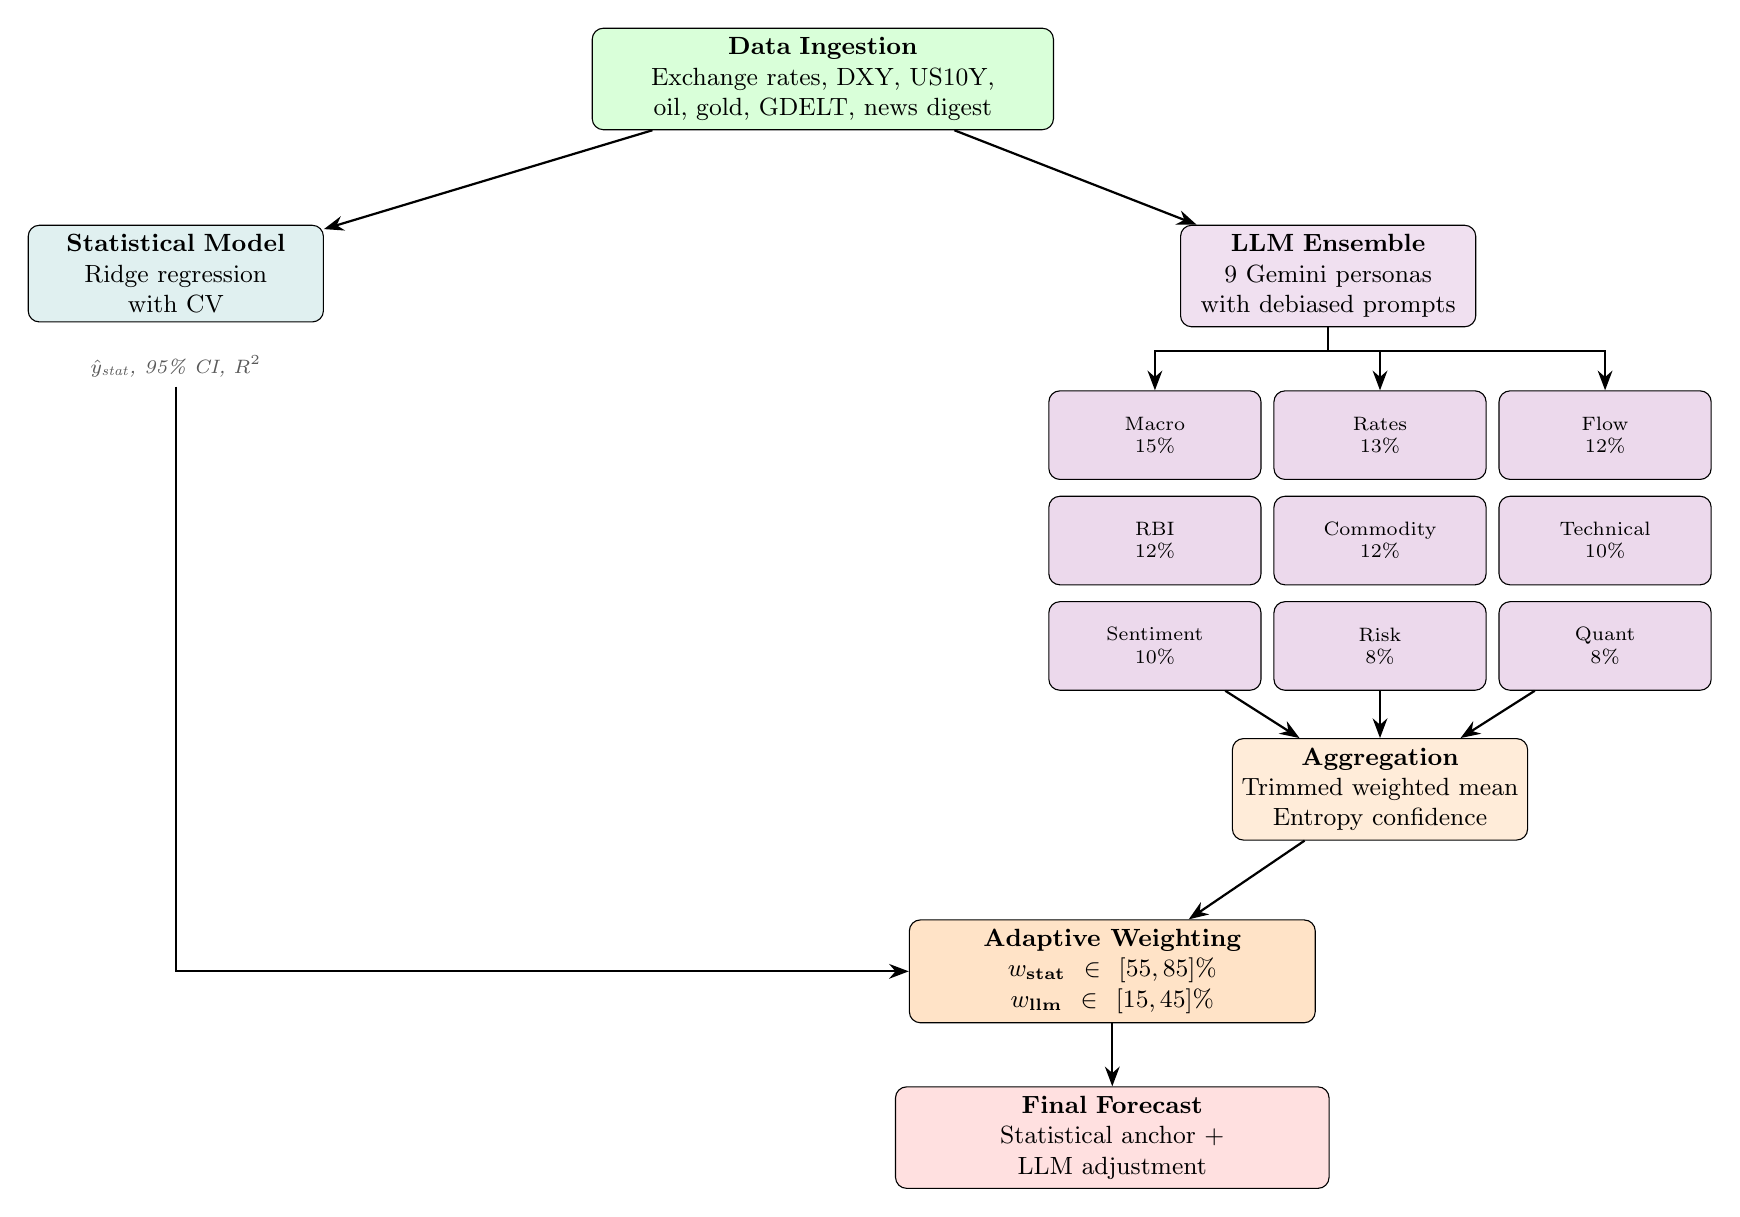
\begin{tikzpicture}[node distance=0.7cm, every node/.style={font=\small}]
    \node[data, text width=16em] (data) {\textbf{Data Ingestion}\\Exchange rates, DXY, US10Y, oil, gold, GDELT, news digest};

    \node[block, below left=1.2cm and 3.4cm of data, fill=teal!12, text width=10em] (stat) {\textbf{Statistical Model}\\Ridge regression\\with CV};
    \node[block, below right=1.2cm and 1.6cm of data, fill=violet!12, text width=10em] (llm) {\textbf{LLM Ensemble}\\9 Gemini personas\\with debiased prompts};

    \node[label, below=0.3cm of stat, text width=10em, align=center] (statout) {$\hat{y}_{\text{stat}}$, 95\% CI, $R^2$};

    \node[persona, below=0.8cm of llm, xshift=-2.2cm] (p1) {Macro\\15\%};
    \node[persona, right=0.15cm of p1] (p2) {Rates\\13\%};
    \node[persona, right=0.15cm of p2] (p3) {Flow\\12\%};
    \node[persona, below=0.2cm of p1] (p4) {RBI\\12\%};
    \node[persona, right=0.15cm of p4] (p5) {Commodity\\12\%};
    \node[persona, right=0.15cm of p5] (p6) {Technical\\10\%};
    \node[persona, below=0.2cm of p4] (p7) {Sentiment\\10\%};
    \node[persona, right=0.15cm of p7] (p8) {Risk\\8\%};
    \node[persona, right=0.15cm of p8] (p9) {Quant\\8\%};

    \node[block, below=0.6cm of p8, fill=orange!15, text width=10em] (agg) {\textbf{Aggregation}\\Trimmed weighted mean\\Entropy confidence};
    \node[phase, below=1cm of agg, xshift=-3.4cm, text width=14em] (adapt) {Adaptive Weighting\\$w_{\text{stat}}\in[55,85]\%$\\$w_{\text{llm}}\in[15,45]\%$};
    \node[output, below=0.8cm of adapt, text width=15em] (final) {\textbf{Final Forecast}\\Statistical anchor +\\LLM adjustment};

    \draw[arrow] (data) -- (stat);
    \draw[arrow] (data) -- (llm);
    \draw[arrow] (llm.south) -- ++(0,-0.3cm) -| (p1.north);
    \draw[arrow] (llm.south) -- ++(0,-0.3cm) -| (p2.north);
    \draw[arrow] (llm.south) -- ++(0,-0.3cm) -| (p3.north);
    \draw[arrow] (p7) -- (agg);
    \draw[arrow] (p8) -- (agg);
    \draw[arrow] (p9) -- (agg);
    \draw[arrow] (statout.south) -- (statout.south |- adapt.west) -- (adapt.west);
    \draw[arrow] (agg) -- (adapt);
    \draw[arrow] (adapt) -- (final);
\end{tikzpicture}}
\caption{Gemini V4 architecture as represented in the repository's historical LLM track. The LLM does not replace the statistical model; it perturbs and annotates it.}
\label{fig:gemini_arch}
\end{figure*}

V4's debiasing techniques are as important as the personas themselves:
\begin{enumerate}[leftmargin=*]
    \item symmetric bull and bear case presentation,
    \item randomized direction order,
    \item explicit confidence intervals and statistical model quality,
    \item persona-level historical accountability,
    \item bias feedback based on prior directional skew,
    \item pip-bounded adjustment magnitudes.
\end{enumerate}

The later repository branches inherit this lesson: persona systems are useful only when they operate as constrained overlays on top of structured quantitative state.

\subsection{\texttt{final phase}: Market-Memory-First Hybrid Forecasting}

The \texttt{final phase} system is the most current engineering-oriented branch in the repository. It departs from the earlier Gemini scripts in three ways.

First, it creates a grouped feature frame spanning technical, macro, master-sentiment, Goldstein, thematic, political, and memory features. Second, it introduces a shared market-memory snapshot that compresses recent history into stable state variables: oil pressure, dollar pressure, carry pressure, India stress, bilateral divergence, event heat, volatility stress, reversal pressure, and a regime label. Third, it evaluates everything under walk-forward backtests with an information embargo, rather than using the most recent price as an implicit shortcut. Concretely, the feature builder predicts a forward target shifted by \texttt{forecast\_horizon\_days + embargo\_days}, so the default task becomes a two-day-gap forecast rather than a trivial persistence exercise.

The persona engine in \texttt{final phase} also differs from the older Gemini branch. Rule personas and LLM personas both consume the same structured market memory, and calibration weights are updated from matured forecast outcomes. This makes the system auditable and branch-comparable in a way the earlier ad hoc scripts were not.

\subsection{TEPC: Topology-Enabled Predictions from Chaos}

TEPC is the most conceptually ambitious branch in the repository. It stops treating USD/INR as a single scalar time series and instead models it as a node in a time-varying macro-geopolitical network. The node universe includes direct market nodes such as INRUSD, DXY, BRENT, GOLD, and US10Y, plus composite nodes such as India sentiment, US sentiment, Goldstein spread, geopolitical risk, and theme pressure.

For each rolling window, TEPC computes a correlation matrix across node shock series, converts correlation into distance,
\begin{equation}
d_{ij} = \sqrt{\frac{1 - \rho_{ij}}{2}},
\end{equation}
and then applies an exponential kernel to obtain a dense adjacency matrix,
\begin{equation}
A_{ij} = \exp\!\left(-\frac{d_{ij}}{\sigma}\right), \qquad A_{ii}=0.
\end{equation}
From the resulting Laplacian $L = D - A$, TEPC extracts degree, density, Fiedler value, spectral entropy, filtration component counts, and target-node adjacency features.

The chaos layer assigns each node a coupled Lorenz oscillator:
\begin{align}
\dot{x} &= \sigma(y - x) - \epsilon(Lx), \\
\dot{y} &= x(\rho - z) - y - 0.35\epsilon(Ly), \\
\dot{z} &= xy - \beta z - 0.15\epsilon(Lz),
\end{align}
with initial conditions derived deterministically from recent volatility, drift, and range position. TEPC then records synchronization, target-node phase response, finite-time Lyapunov-style divergence, and coupling response as predictive features. A strict configuration further enforces \texttt{response\_lag\_days = 2}, explicitly preventing access to the target day's immediately prior price. This makes TEPC the repository's clearest attempt to escape trivial lag-copying.

% ============================================================
% 5. EXPERIMENTAL SETUP
% ============================================================
\section{Experimental Setup}

\subsection{Branch-Specific Evaluation Protocols}

Because the repository is a research program rather than one frozen benchmark, each branch uses the evaluation protocol most appropriate to its question. Table~\ref{tab:protocols} summarizes the main ones used in this paper.

\begin{table*}[t]
\centering
\small
\caption{Evaluation protocols used across major branches.}
\label{tab:protocols}
\resizebox{\textwidth}{!}{%
\begin{tabular}{p{2.3cm}p{4.0cm}p{3.5cm}p{4.4cm}p{3.2cm}}
\toprule
\textbf{Branch} & \textbf{Target} & \textbf{Evaluation Window} & \textbf{Primary Metrics} & \textbf{Key Design Constraint} \\
\midrule
Phase C & IMF$_3$ danger-day classification and 3-class direction & Chronological 80/20 split over Phase-B merged data & precision, recall, F1, accuracy, tuned threshold & Top 20\% IMF$_3$ defines ``danger'' \\
GARCH & Volatility fit and hybrid return modeling & Full saved branch outputs on 2025 daily data & log-likelihood, AIC, BIC, feature importance & Asymmetry and persistence are first-class outputs \\
Ensemble / ultimate model comparison & Next-period point forecast comparison & Saved ensemble holdout artifacts & RMSE, MAE, $R^2$, final optimized weights & Many model families are compared under the same branch \\
Gemini V3/V4 & Next-day price and direction & 2023 full-year saved summary (260 rows) + Jan 2026 live test (21 rows) & mean absolute error \%, sign accuracy, weight ranges & Statistical anchor plus persona adjustment \\
\texttt{final phase} & Future price, return, direction under walk-forward evaluation & 100-day and 30-day walk-forward backtests & MAE price, RMSE price, MAE return, directional accuracy, sign-F1 & Effective two-day target gap via horizon + embargo \\
TEPC strict raw & Breakout, forward return, near-term volatility & 80-day walk-forward strict raw-GDELT run & breakout accuracy, macro-F1, MAE return, volatility MAE & Response lag = 2 days; no flat lag-copying \\
TEPC livepull & Same TEPC tasks on extended node feed & 100-day livepull walk-forward run & breakout accuracy, macro-F1, MAE return & Optional cross-FX and live-news nodes retained when coverage permits \\
\bottomrule
\end{tabular}}
\end{table*}

\subsection{Implemented Baselines}

The repository contains the following implemented comparison families:
\begin{itemize}[leftmargin=*]
    \item classical time-series baselines: ARIMA, SARIMA, Holt--Winters, Theta;
    \item volatility baselines: GARCH, GJR-GARCH, EGARCH;
    \item ML baselines: OLS, Ridge, Random Forest, XGBoost, Gradient Boosting;
    \item deep learning baselines: LSTM, GRU, Attention;
    \item scenario baselines: GBM, jump diffusion, sentiment-augmented drift, regime switching;
    \item LLM baselines and ablations: Gemini V3, Gemini V4, rule personas, memory-only, and later multi-provider LLM persona matrices;
    \item topology/chaos ablations: macro baseline, topology-only, chaos-only, topology+chaos, TEPC full, persona-only, and TEPC persona blends.
\end{itemize}

No saved ARDL or DMI benchmark outputs were found in the repository snapshot. We therefore do not fabricate ARDL/DMI rows in the result tables. Where the user requested such comparisons, we interpret the scientific intent as comparing against the strongest available implemented econometric and technical baselines.

% ============================================================
% 6. RESULTS
% ============================================================
\section{Results}

\subsection{Raw Aggregate News is Weak; Structured and Lagged News is Better}

The first clear repository-wide lesson is negative: raw aggregate news statistics are not enough. Goldstein aggregated directly against IMF$_3$ is almost useless; naive political-news enhancement can even worsen regression models. Only after thematic filtering, lag analysis, and stateful feature engineering does signal become usable.

\begin{table*}[t]
\centering
\small
\caption{Early-stage signal discovery across the repository.}
\label{tab:signal_discovery}
\begin{tabular}{p{4.2cm}p{3.0cm}p{8.0cm}}
\toprule
\textbf{Artifact / Statistic} & \textbf{Value} & \textbf{Interpretation} \\
\midrule
Goldstein vs.\ IMF$_3$ correlation & $0.009965$ & Raw bilateral Goldstein aggregation alone has negligible direct relationship with the decomposed noise target. \\
US average tone vs.\ USD/INR correlation & $0.1639$ & Cross-country tone carries weak but nonzero information; it is not sufficient as a standalone predictor. \\
Phase-B \texttt{Tone\_Economy} vs.\ IMF$_3$ & $-0.1466$ (p $= 0.0194$) & Theme-filtered economic tone becomes statistically meaningful once irrelevant articles are removed. \\
Meaningful-pattern event count correlation with volatility & $-0.1294$ & Event density helps characterize abnormal movement regimes. \\
Peak Goldstein lag & 9 days & The strongest Goldstein relationship appears with delay rather than contemporaneously. \\
Peak tone lag & 12 days & Tone shifts also appear delayed, supporting lagged rather than same-day feature design. \\
Political-news enhancement on RF/XGBoost & RMSE worsened by 1.18\% / 1.78\% & Naive injection of political features can degrade price regressors when decomposition and lag structure are absent. \\
\bottomrule
\end{tabular}
\end{table*}

\begin{figure*}[t]
\centering
\begin{subfigure}[t]{0.48\textwidth}
    \centering
    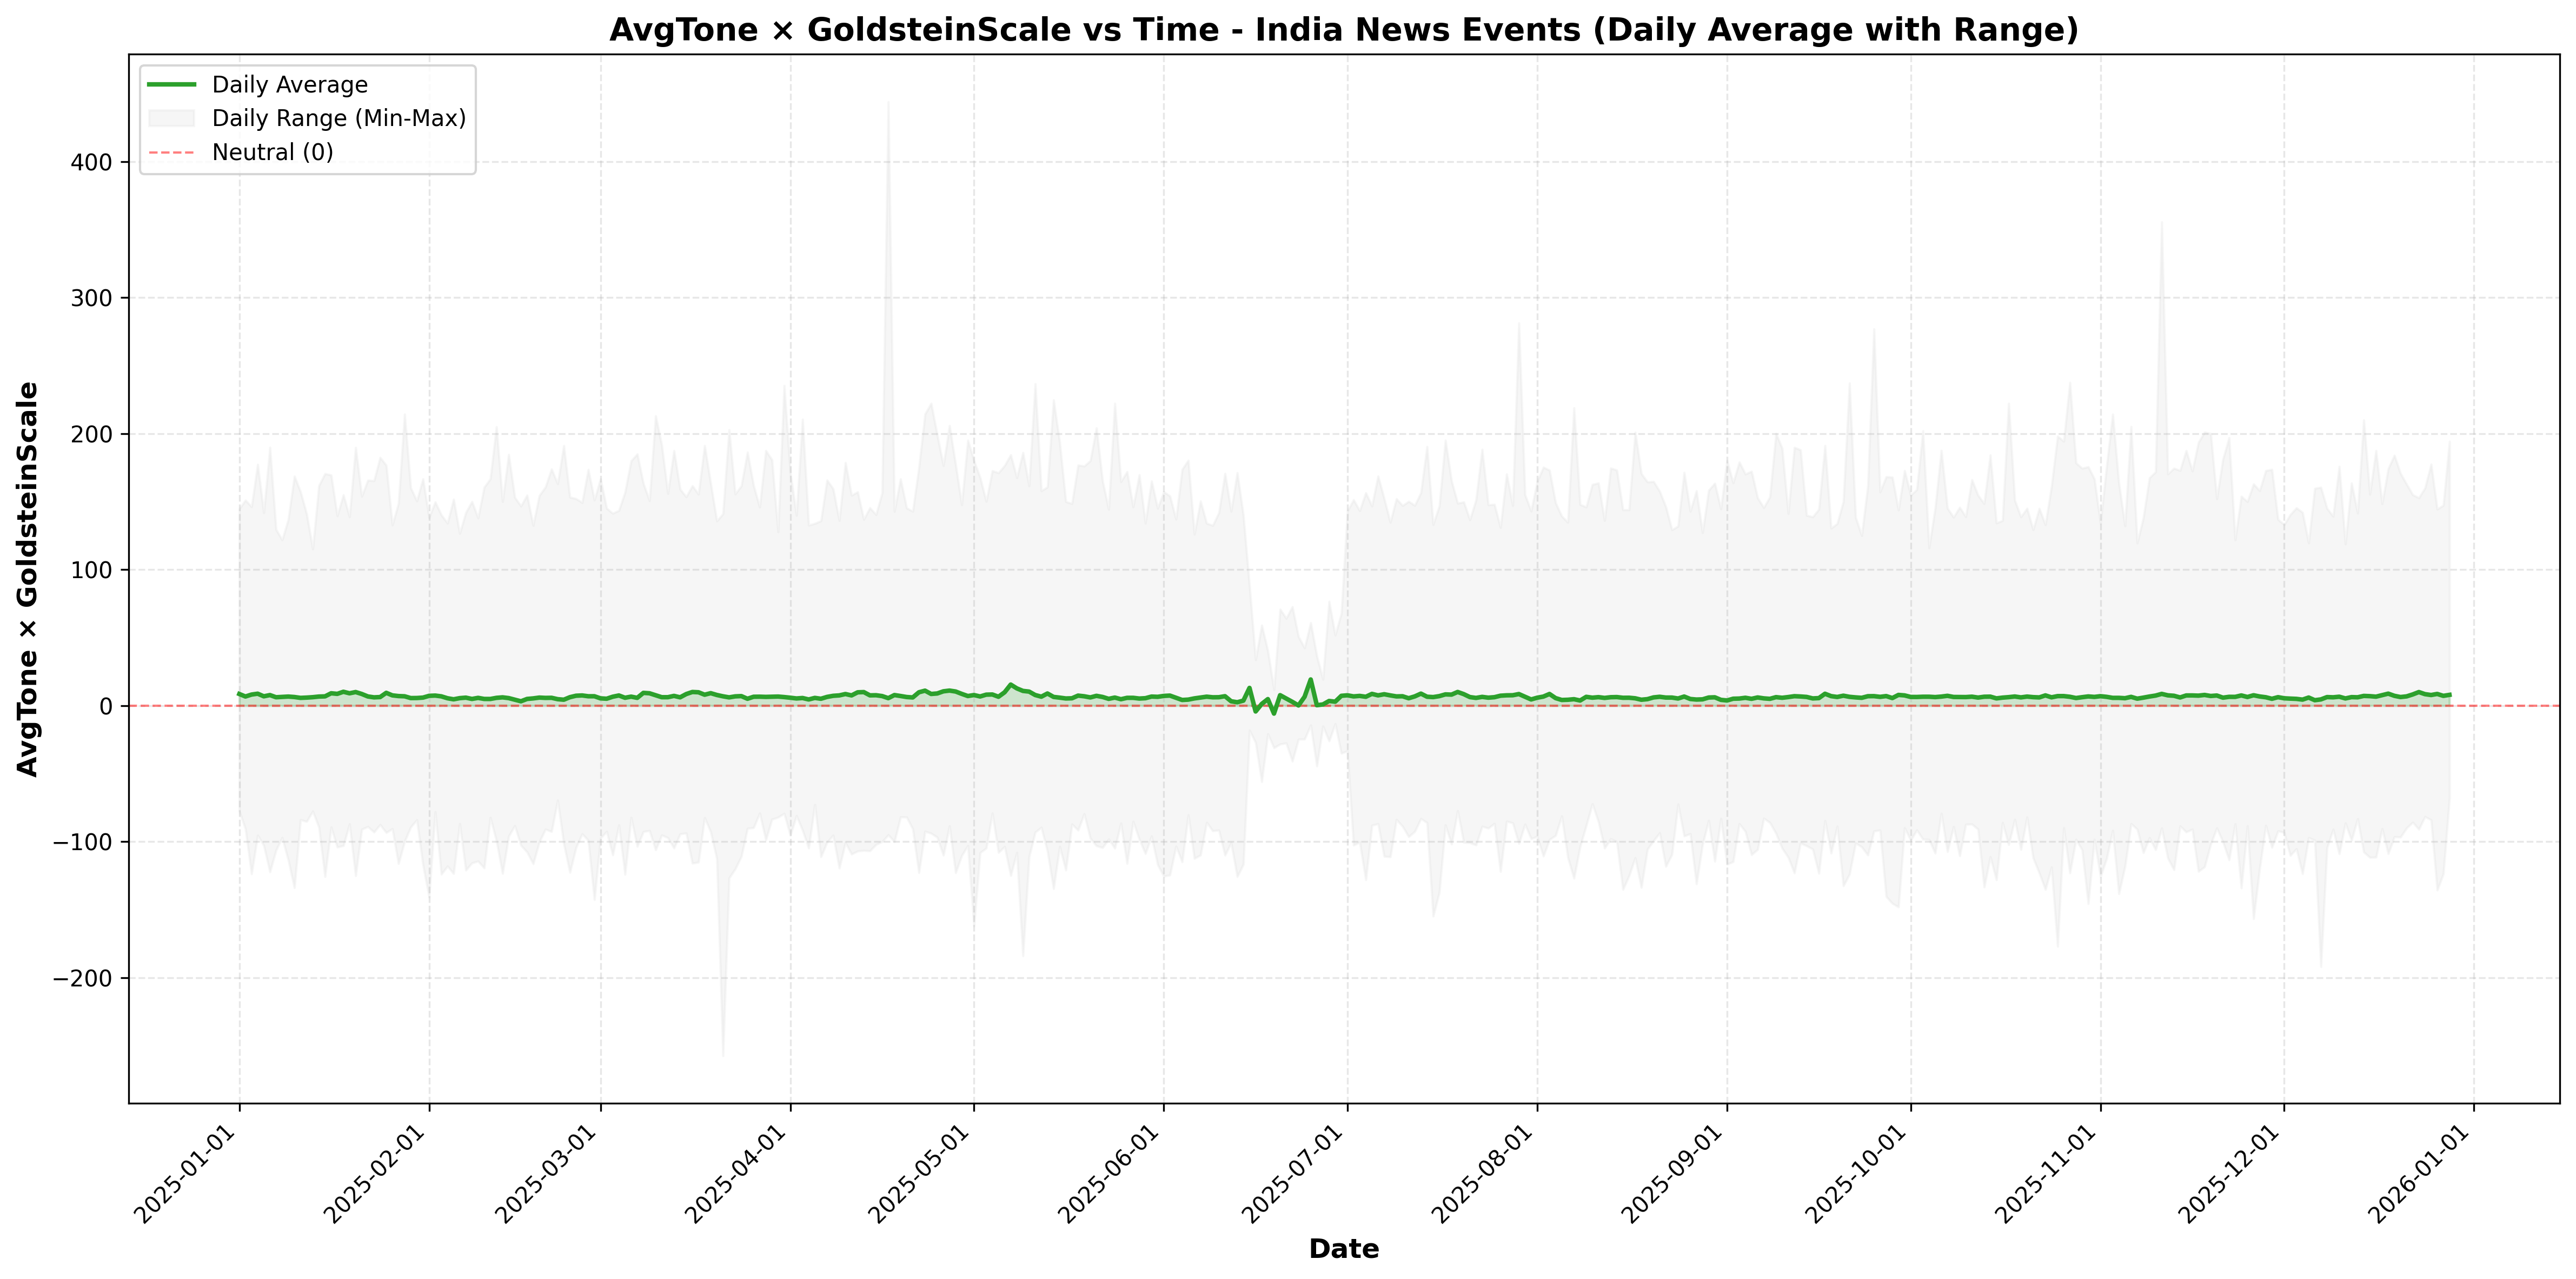
\includegraphics[width=\linewidth]{lead_lag.png}
    \caption{Lead-lag visualization used in the early research track.}
\end{subfigure}
\hfill
\begin{subfigure}[t]{0.48\textwidth}
    \centering
    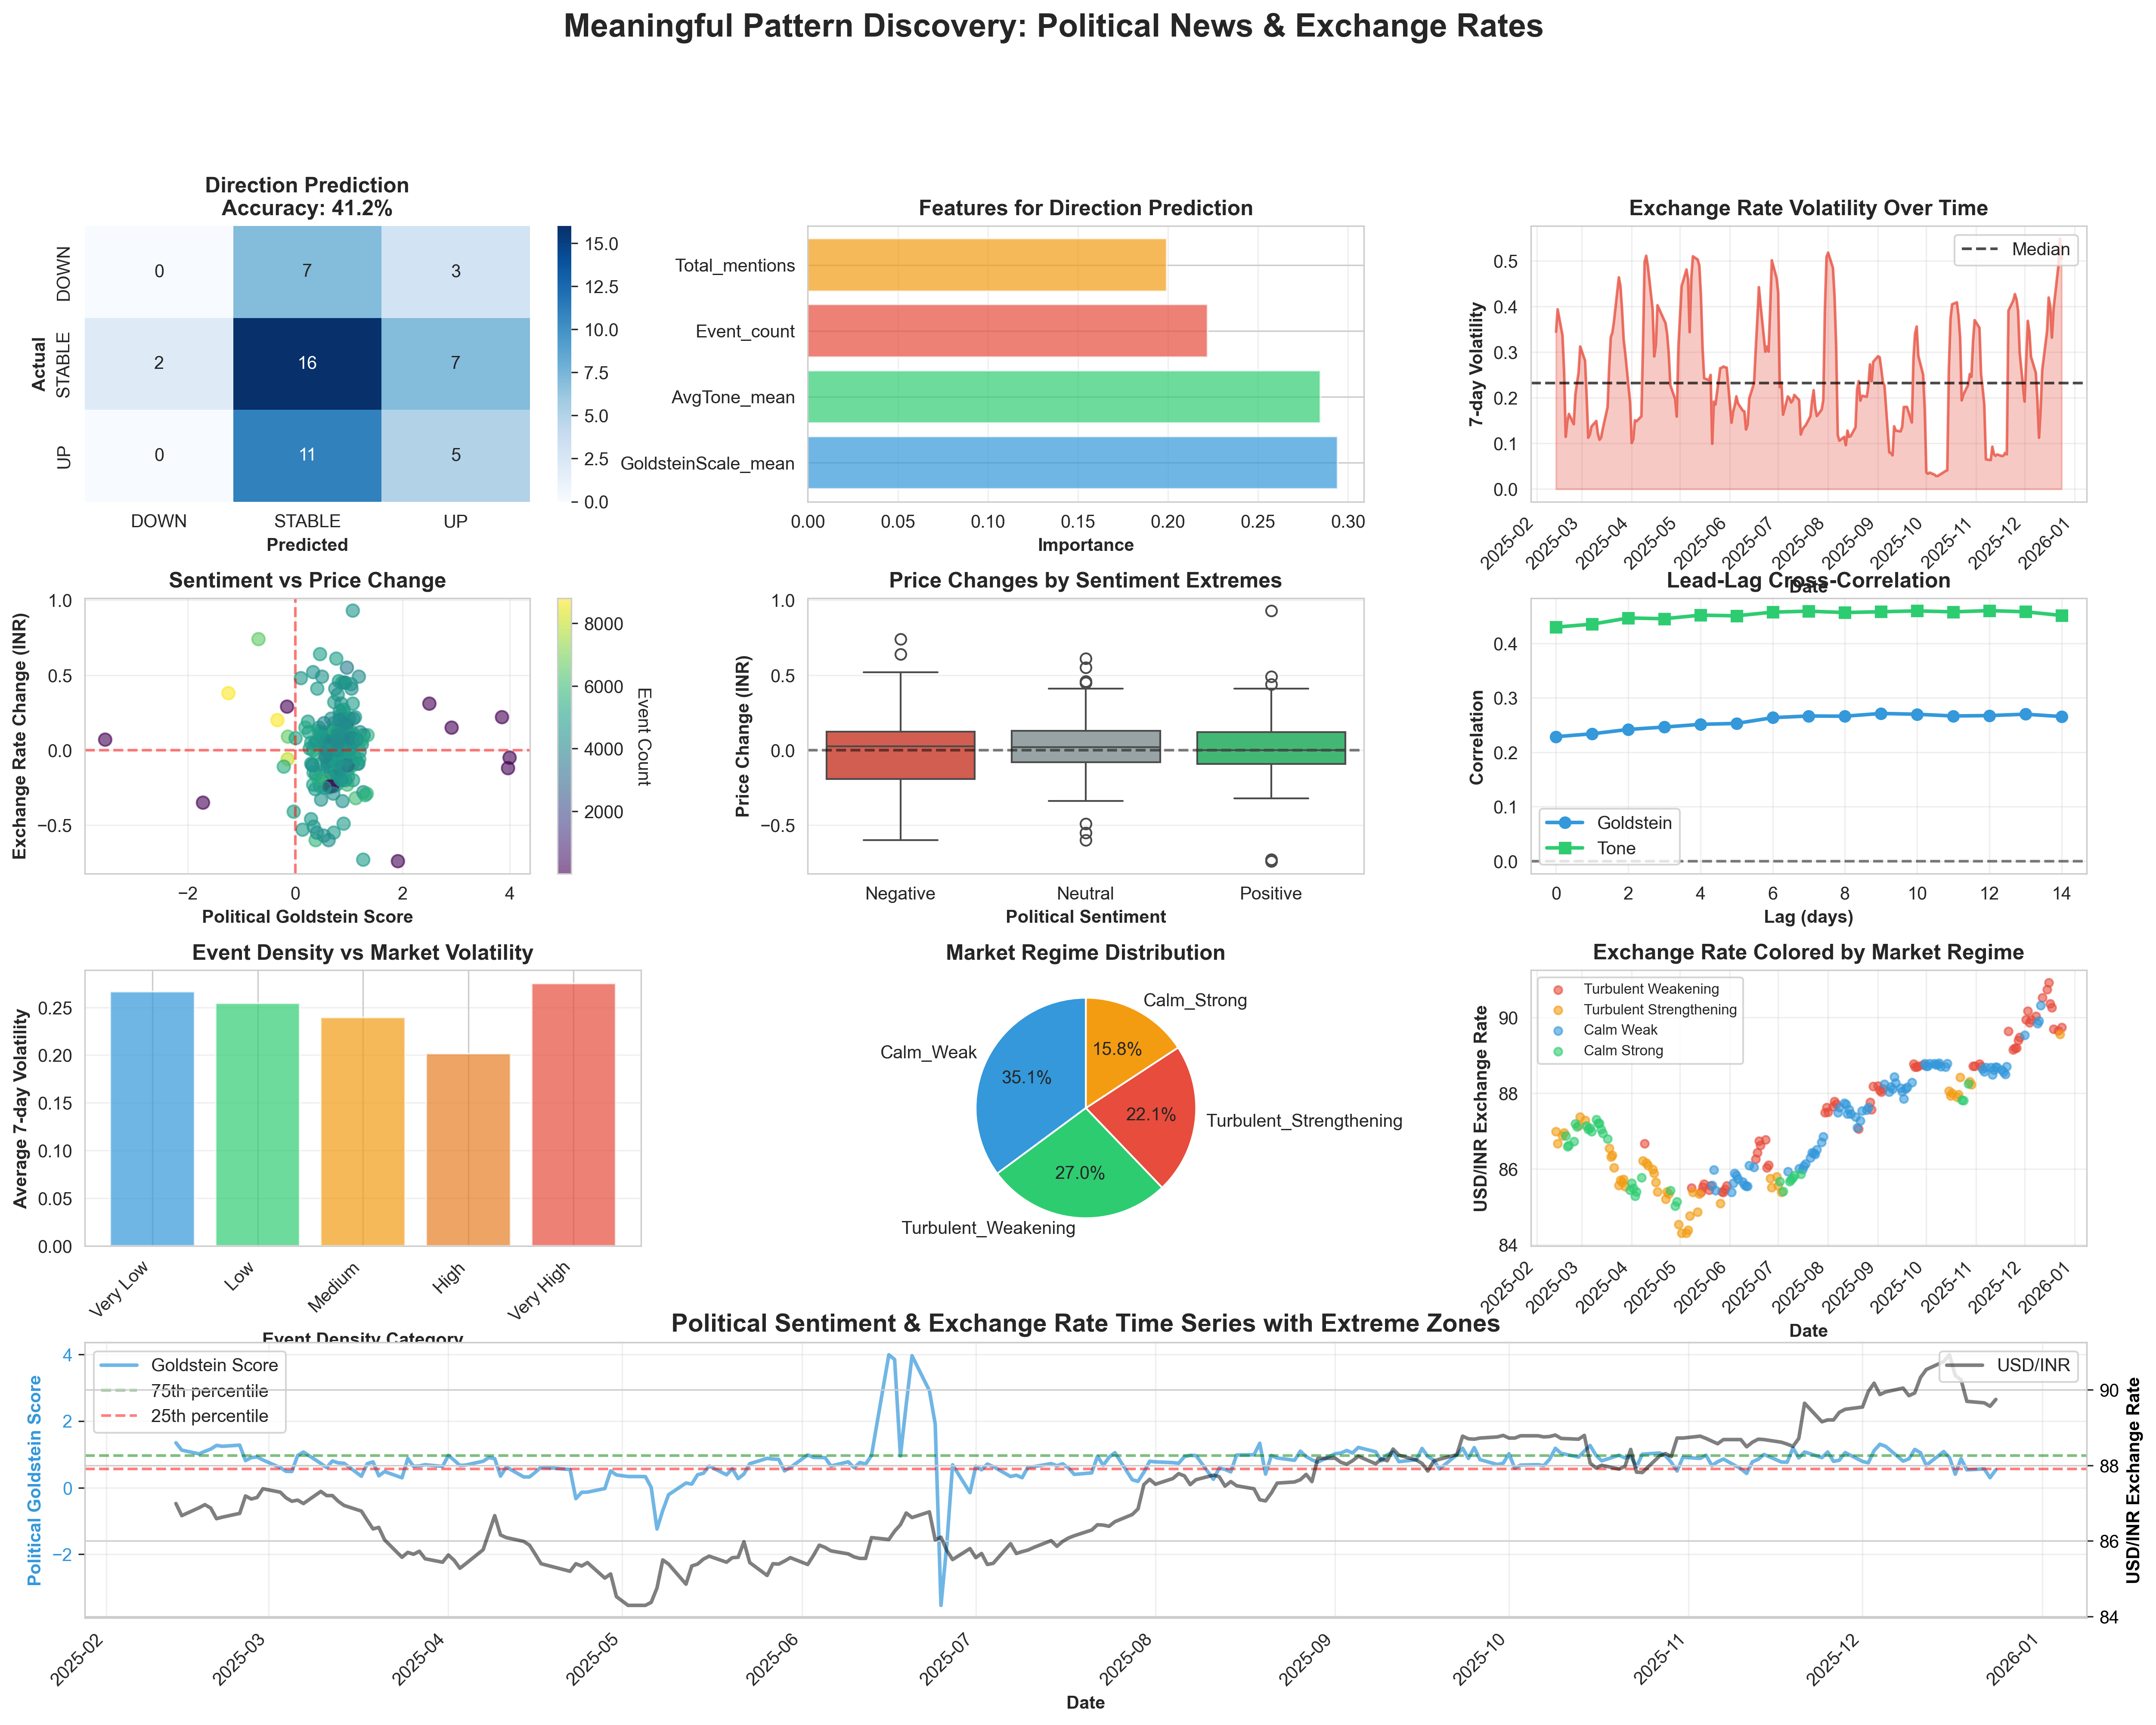
\includegraphics[width=\linewidth]{meaningful_patterns.png}
    \caption{Broader meaningful-pattern analysis across direction, volatility, and regimes.}
\end{subfigure}
\caption{The strongest signal in the early repository is delayed and regime-like, not a contemporaneous one-shot news-to-price mapping.}
\label{fig:leadlag}
\end{figure*}

This is precisely why the Indian FX market is poorly suited to simplistic direct application of many models. USD/INR does not reward a ``feed in raw sentiment, predict tomorrow's price'' workflow. It requires filtering, alignment, and delayed-state representation.

\subsection{Phase C: Danger-Day Classification Works Better Than Direct Price Regression}

The saved Phase-C artifacts support the repository's shift toward classification. Danger days are rare, so precision matters more than aggregate accuracy. At the F1-optimized threshold of 0.38, the classifier achieves a substantial improvement over a random 20\% precision baseline.

\begin{table}[t]
\centering
\small
\caption{Phase-C danger-day classification results on the saved test split (73 days).}
\label{tab:danger}
\begin{tabular}{lr}
\toprule
\textbf{Statistic} & \textbf{Value} \\
\midrule
True positives & 12 \\
False positives & 18 \\
True negatives & 32 \\
False negatives & 11 \\
\midrule
Precision & 40\% \\
Recall & 52\% \\
F1-score & 0.45 \\
Accuracy & 60\% \\
Optimal threshold & 0.38 \\
\bottomrule
\end{tabular}
\end{table}

The broader meaningful-pattern analysis also reports 41.2\% accuracy on UP/DOWN/STABLE directional classification, again above the naive baseline. The core result is not that the model predicts exact prices particularly well; it does not. The result is that state-dependent volatility and directional stress are tractable.

\begin{figure*}[t]
\centering
\begin{subfigure}[t]{0.48\textwidth}
    \centering
    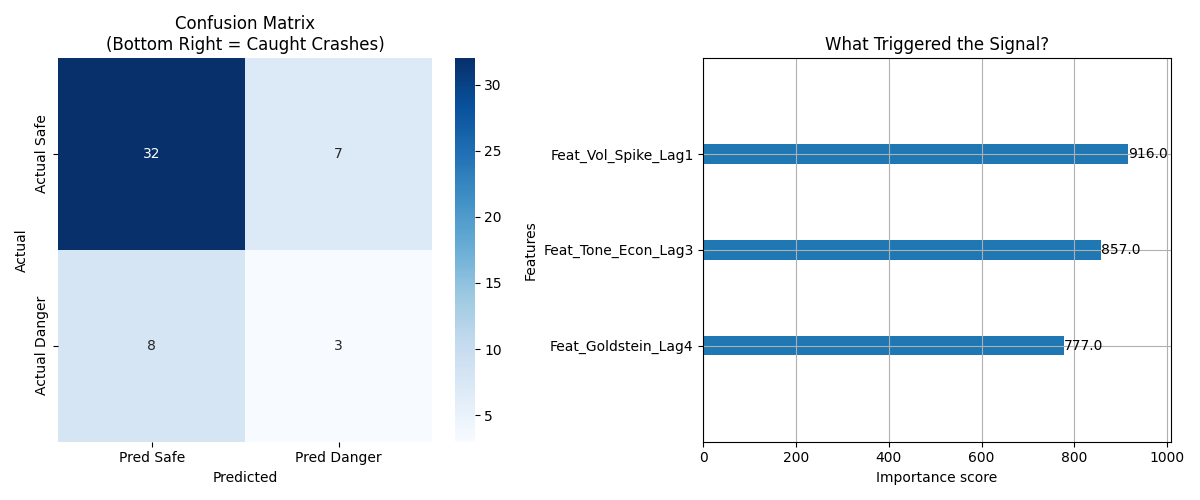
\includegraphics[width=\linewidth]{phase_c_classifier.png}
    \caption{Classifier performance panel.}
\end{subfigure}
\hfill
\begin{subfigure}[t]{0.48\textwidth}
    \centering
    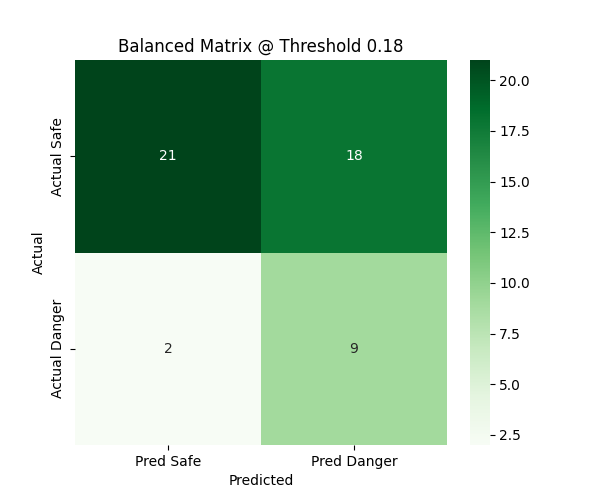
\includegraphics[width=\linewidth]{phase_c_confusion.png}
    \caption{Balanced confusion matrix at the tuned threshold.}
\end{subfigure}
\caption{Phase-C classification results. The practical value lies in risk flagging rather than exact valuation.}
\label{fig:phasec}
\end{figure*}

\subsection{EGARCH Remains Useful, but the Large Ensemble Exposes Many Model Failures}

Table~\ref{tab:garch_family} shows that EGARCH is the strongest of the repository's GARCH-family fits under the saved AIC/BIC comparison.

\begin{table}[t]
\centering
\small
\caption{GARCH-family comparison from \texttt{GARCH/output/garch\_comparison.csv}.}
\label{tab:garch_family}
\begin{tabular}{lcccc}
\toprule
\textbf{Model} & \textbf{Log-Lik.} & \textbf{AIC} & \textbf{BIC} & \textbf{Asymmetry} \\
\midrule
EGARCH & $-23.166$ & \textbf{60.331} & \textbf{85.037} & 0.2017 \\
GARCH & $-24.225$ & 60.450 & 81.626 & 0.0000 \\
GJR-GARCH & $-23.678$ & 61.356 & 86.062 & $-0.2519$ \\
\bottomrule
\end{tabular}
\end{table}

The hybrid branch's top XGBoost feature importances are also informative: \texttt{Realized\_Vol\_20d} dominates at 27.5\%, followed by \texttt{India\_Avg\_Goldstein} at 15.8\%, \texttt{DTWEXBGS} at 9.6\%, and \texttt{Goldstein\_Avg} at 8.2\%. This is economically plausible. Volatility structure still matters most, but bilateral event pressure and dollar conditions are meaningful secondary drivers.

\begin{figure*}[t]
\centering
\begin{subfigure}[t]{0.48\textwidth}
    \centering
    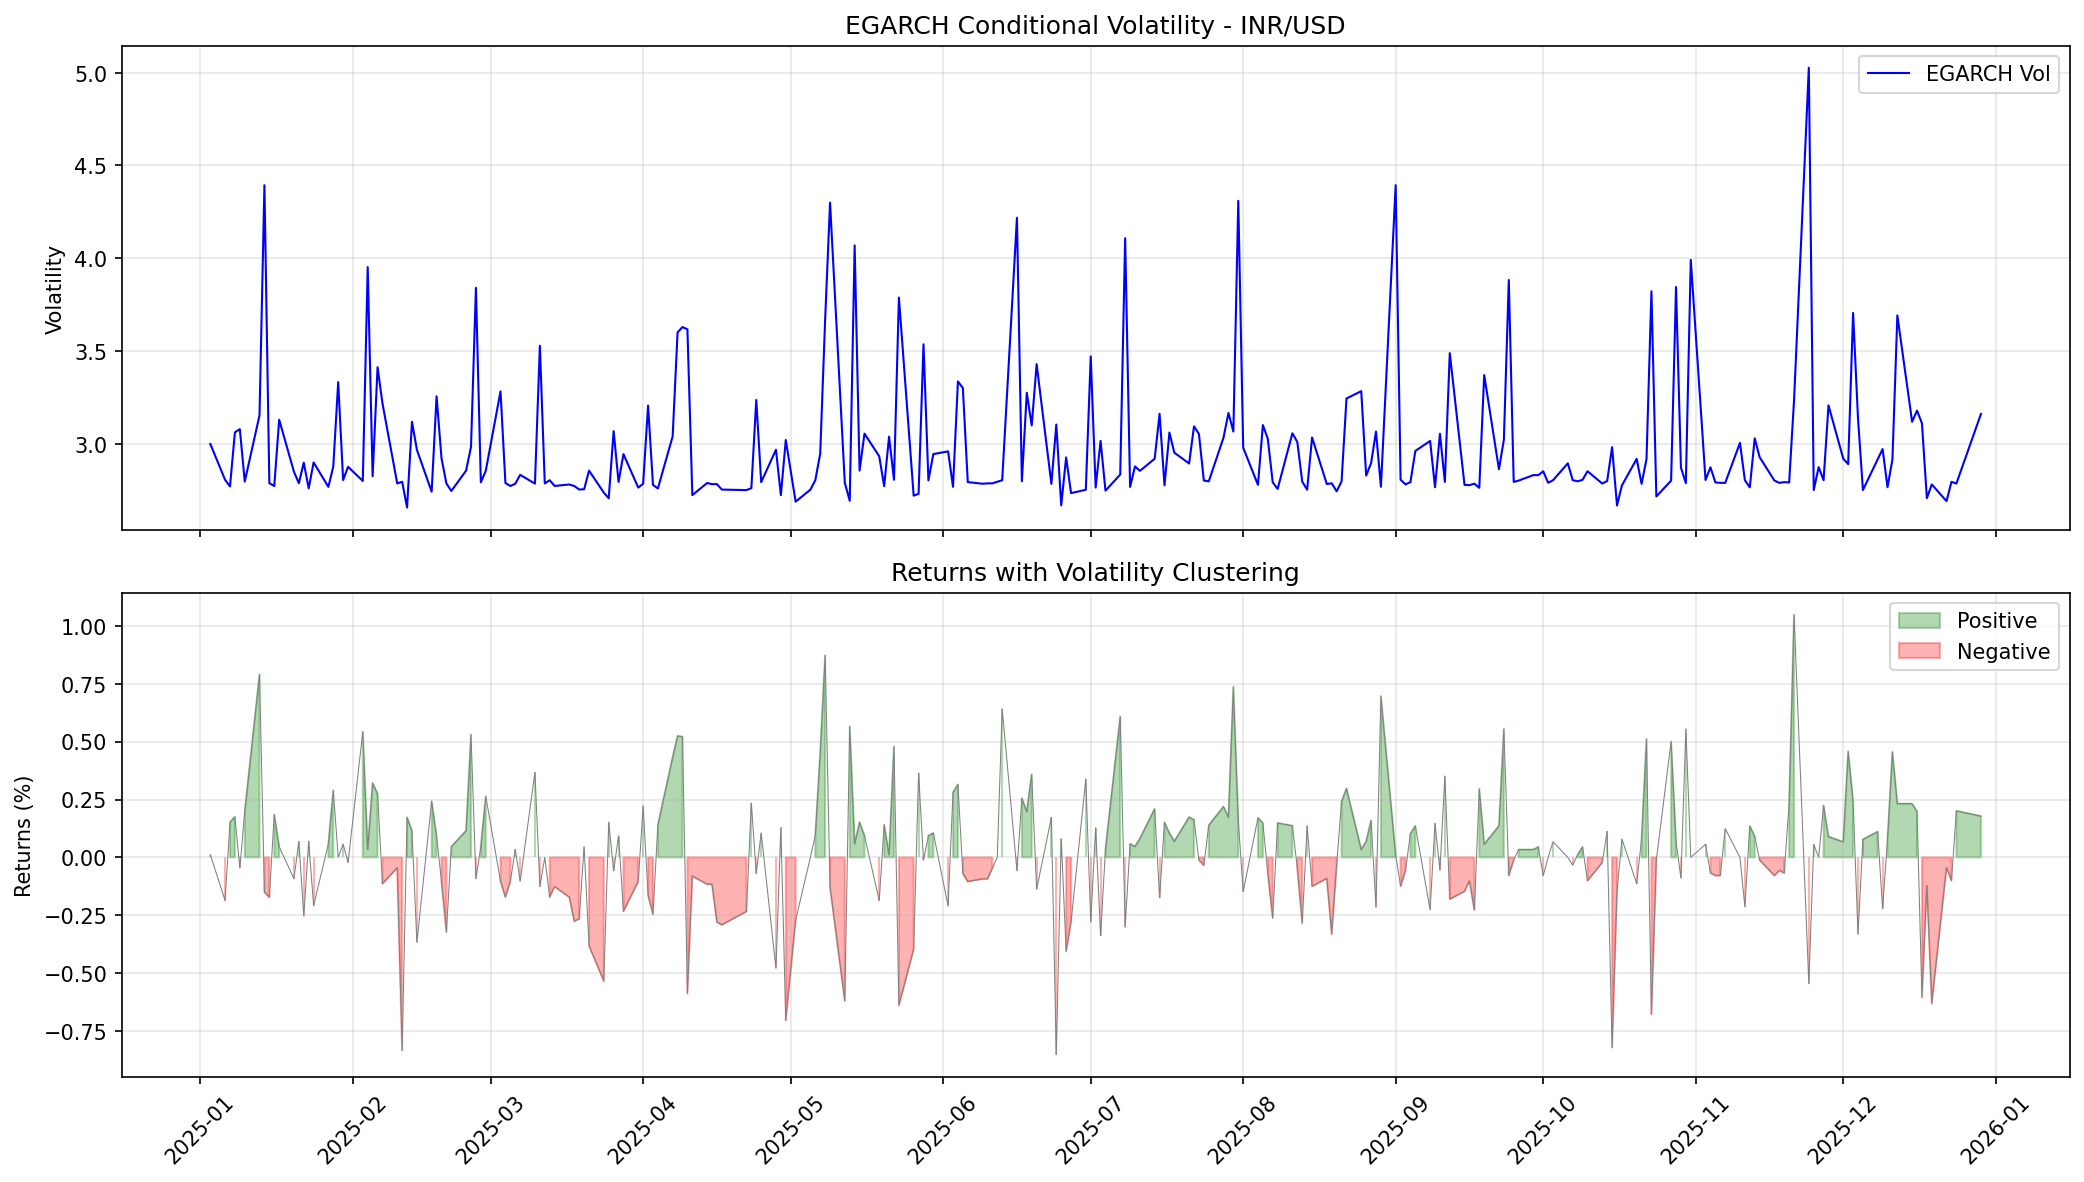
\includegraphics[width=\linewidth]{garch_volatility.png}
    \caption{EGARCH conditional volatility dynamics.}
\end{subfigure}
\hfill
\begin{subfigure}[t]{0.48\textwidth}
    \centering
    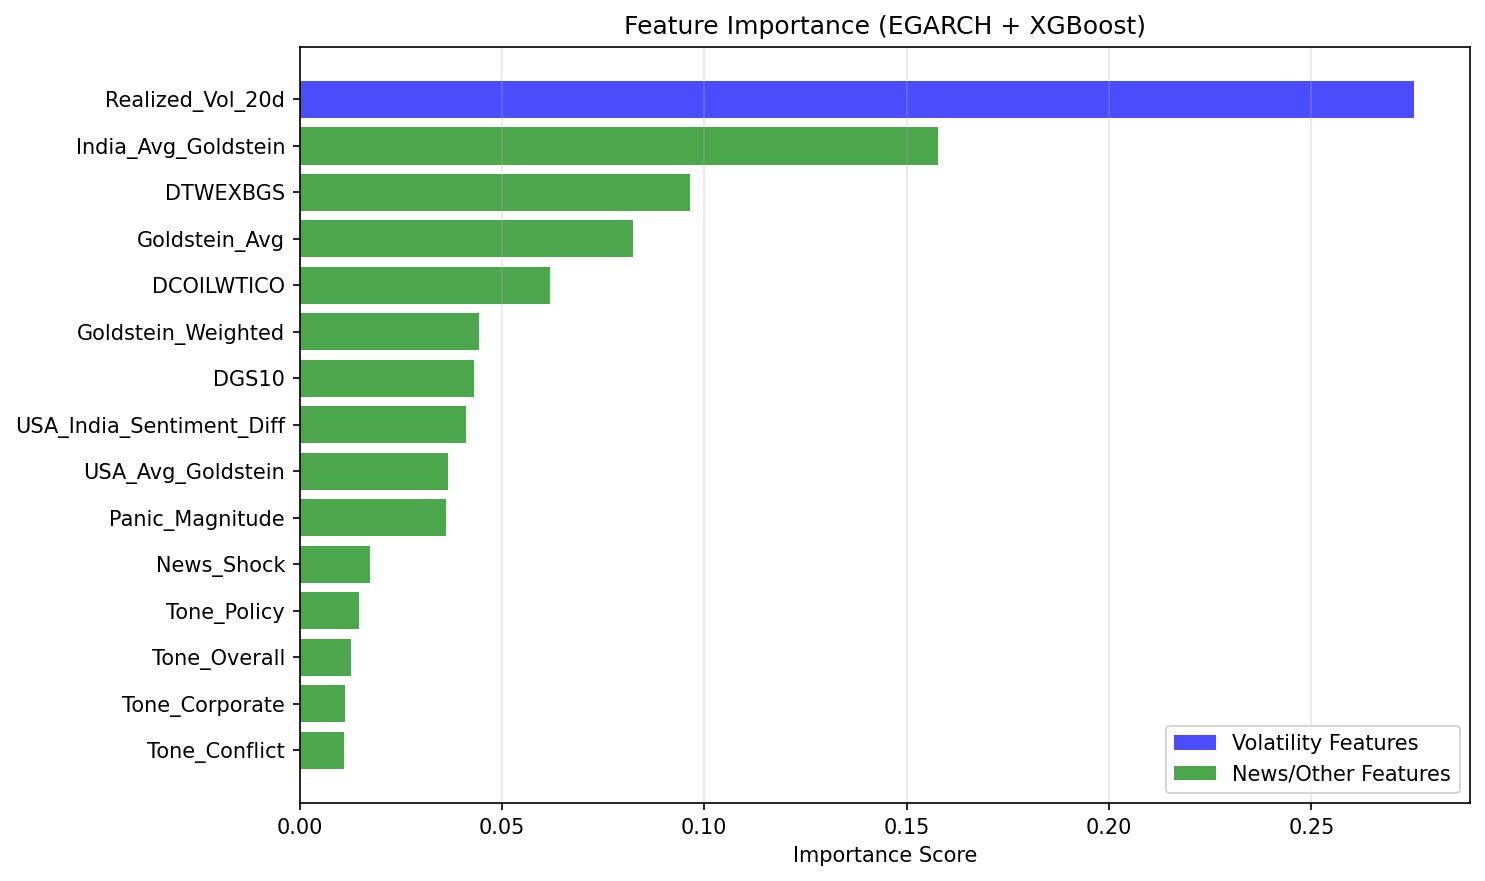
\includegraphics[width=\linewidth]{garch_feature_importance.png}
    \caption{Hybrid EGARCH + XGBoost feature importance.}
\end{subfigure}
\caption{The GARCH branch remains valuable as a volatility and feature-prior engine, even when direct point forecasting remains difficult.}
\label{fig:garch}
\end{figure*}

The ensemble branch reinforces the same lesson even more strongly: many sophisticated models do not survive the task. Table~\ref{tab:ultimate_models} reports selected models from the saved ultimate ensemble comparison.

\begin{table*}[t]
\centering
\small
\caption{Selected models from \texttt{ensemble\_model/output/ultimate\_model\_metrics.csv}.}
\label{tab:ultimate_models}
\resizebox{\textwidth}{!}{%
\begin{tabular}{lccc}
\toprule
\textbf{Model} & \textbf{RMSE} & \textbf{MAE} & \textbf{$R^2$} \\
\midrule
MA\_Momentum & \textbf{0.4950} & \textbf{0.3980} & \textbf{0.5711} \\
Mini\_Ensemble & 0.5673 & 0.4442 & 0.4366 \\
GARCH & 0.5939 & 0.4594 & 0.3826 \\
Monte\_Carlo & 0.6473 & 0.4898 & 0.2666 \\
Theta & 0.6685 & 0.4980 & 0.2178 \\
GDELT\_Ridge & 0.7229 & 0.6270 & 0.0853 \\
VMD\_Trend & 1.0036 & 0.8247 & $-0.7630$ \\
ARIMA & 1.1505 & 0.8949 & $-1.3168$ \\
SARIMA & 1.1574 & 0.9022 & $-1.3448$ \\
GRU & 1.1580 & 0.9029 & $-1.3472$ \\
LSTM & 1.1914 & 0.9282 & $-1.4844$ \\
Attention & 2.6716 & 2.5081 & $-11.4933$ \\
Gemini\_Adjusted & 6.5674 & 6.5435 & $-74.4936$ \\
\bottomrule
\end{tabular}}
\end{table*}

The optimized ensemble weights collapse to a highly interpretable solution: 95.45\% \texttt{MA\_Momentum} and 4.55\% \texttt{GDELT\_Ridge}, with effectively zero weight on the rest. This is the clearest repository-level evidence that the Indian FX market is not hospitable to many off-the-shelf direct point-prediction models. Even SARIMA, the specific baseline requested by the user, is decisively outperformed here.

\subsection{Monte Carlo is Best Used as a Distributional Risk Engine}

The Monte Carlo branch is most valuable when treated as a scenario system. Table~\ref{tab:montecarlo} summarizes the 30-day saved forecast distribution statistics.

\begin{table}[t]
\centering
\small
\caption{Thirty-day Monte Carlo forecast statistics from \texttt{monte\_carlo\_statistics.csv}.}
\label{tab:montecarlo}
\begin{tabular}{lcccc}
\toprule
\textbf{Model} & \textbf{Median} & \textbf{Std} & \textbf{5th Pctl.} & \textbf{95th Pctl.} \\
\midrule
Standard GBM & 90.446 & 1.390 & 88.172 & 92.740 \\
Regime-Switching & \textbf{90.370} & \textbf{1.336} & 88.232 & 92.618 \\
Jump Diffusion & 87.260 & 3.940 & 80.714 & 93.610 \\
Sentiment-Augmented & 91.235 & 1.398 & 88.950 & 93.528 \\
\bottomrule
\end{tabular}
\end{table}

The regime-switching specification is the most balanced saved variant: it preserves uncertainty, avoids the excessive dispersion of jump diffusion, and produces a plausible central trajectory for risk management.

\begin{figure*}[t]
\centering
\begin{subfigure}[t]{0.48\textwidth}
    \centering
    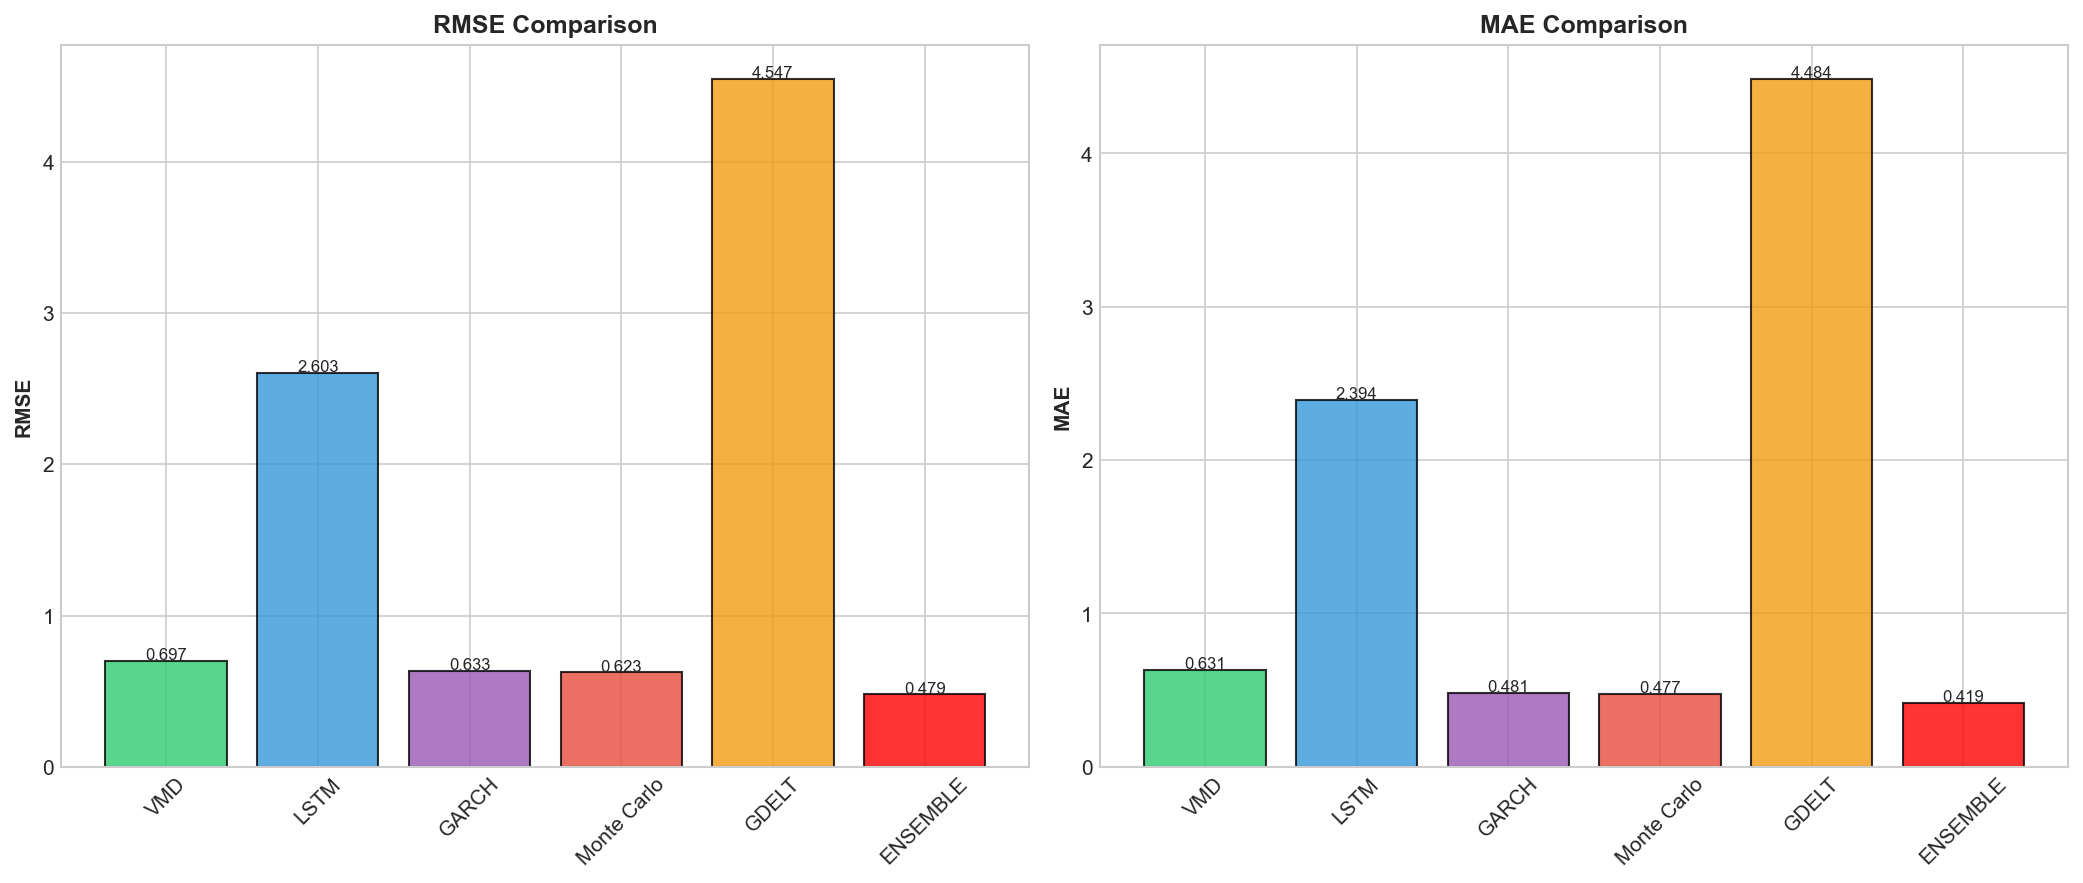
\includegraphics[width=\linewidth]{ensemble_model_comparison.png}
    \caption{Intermediate ensemble comparison output.}
\end{subfigure}
\hfill
\begin{subfigure}[t]{0.48\textwidth}
    \centering
    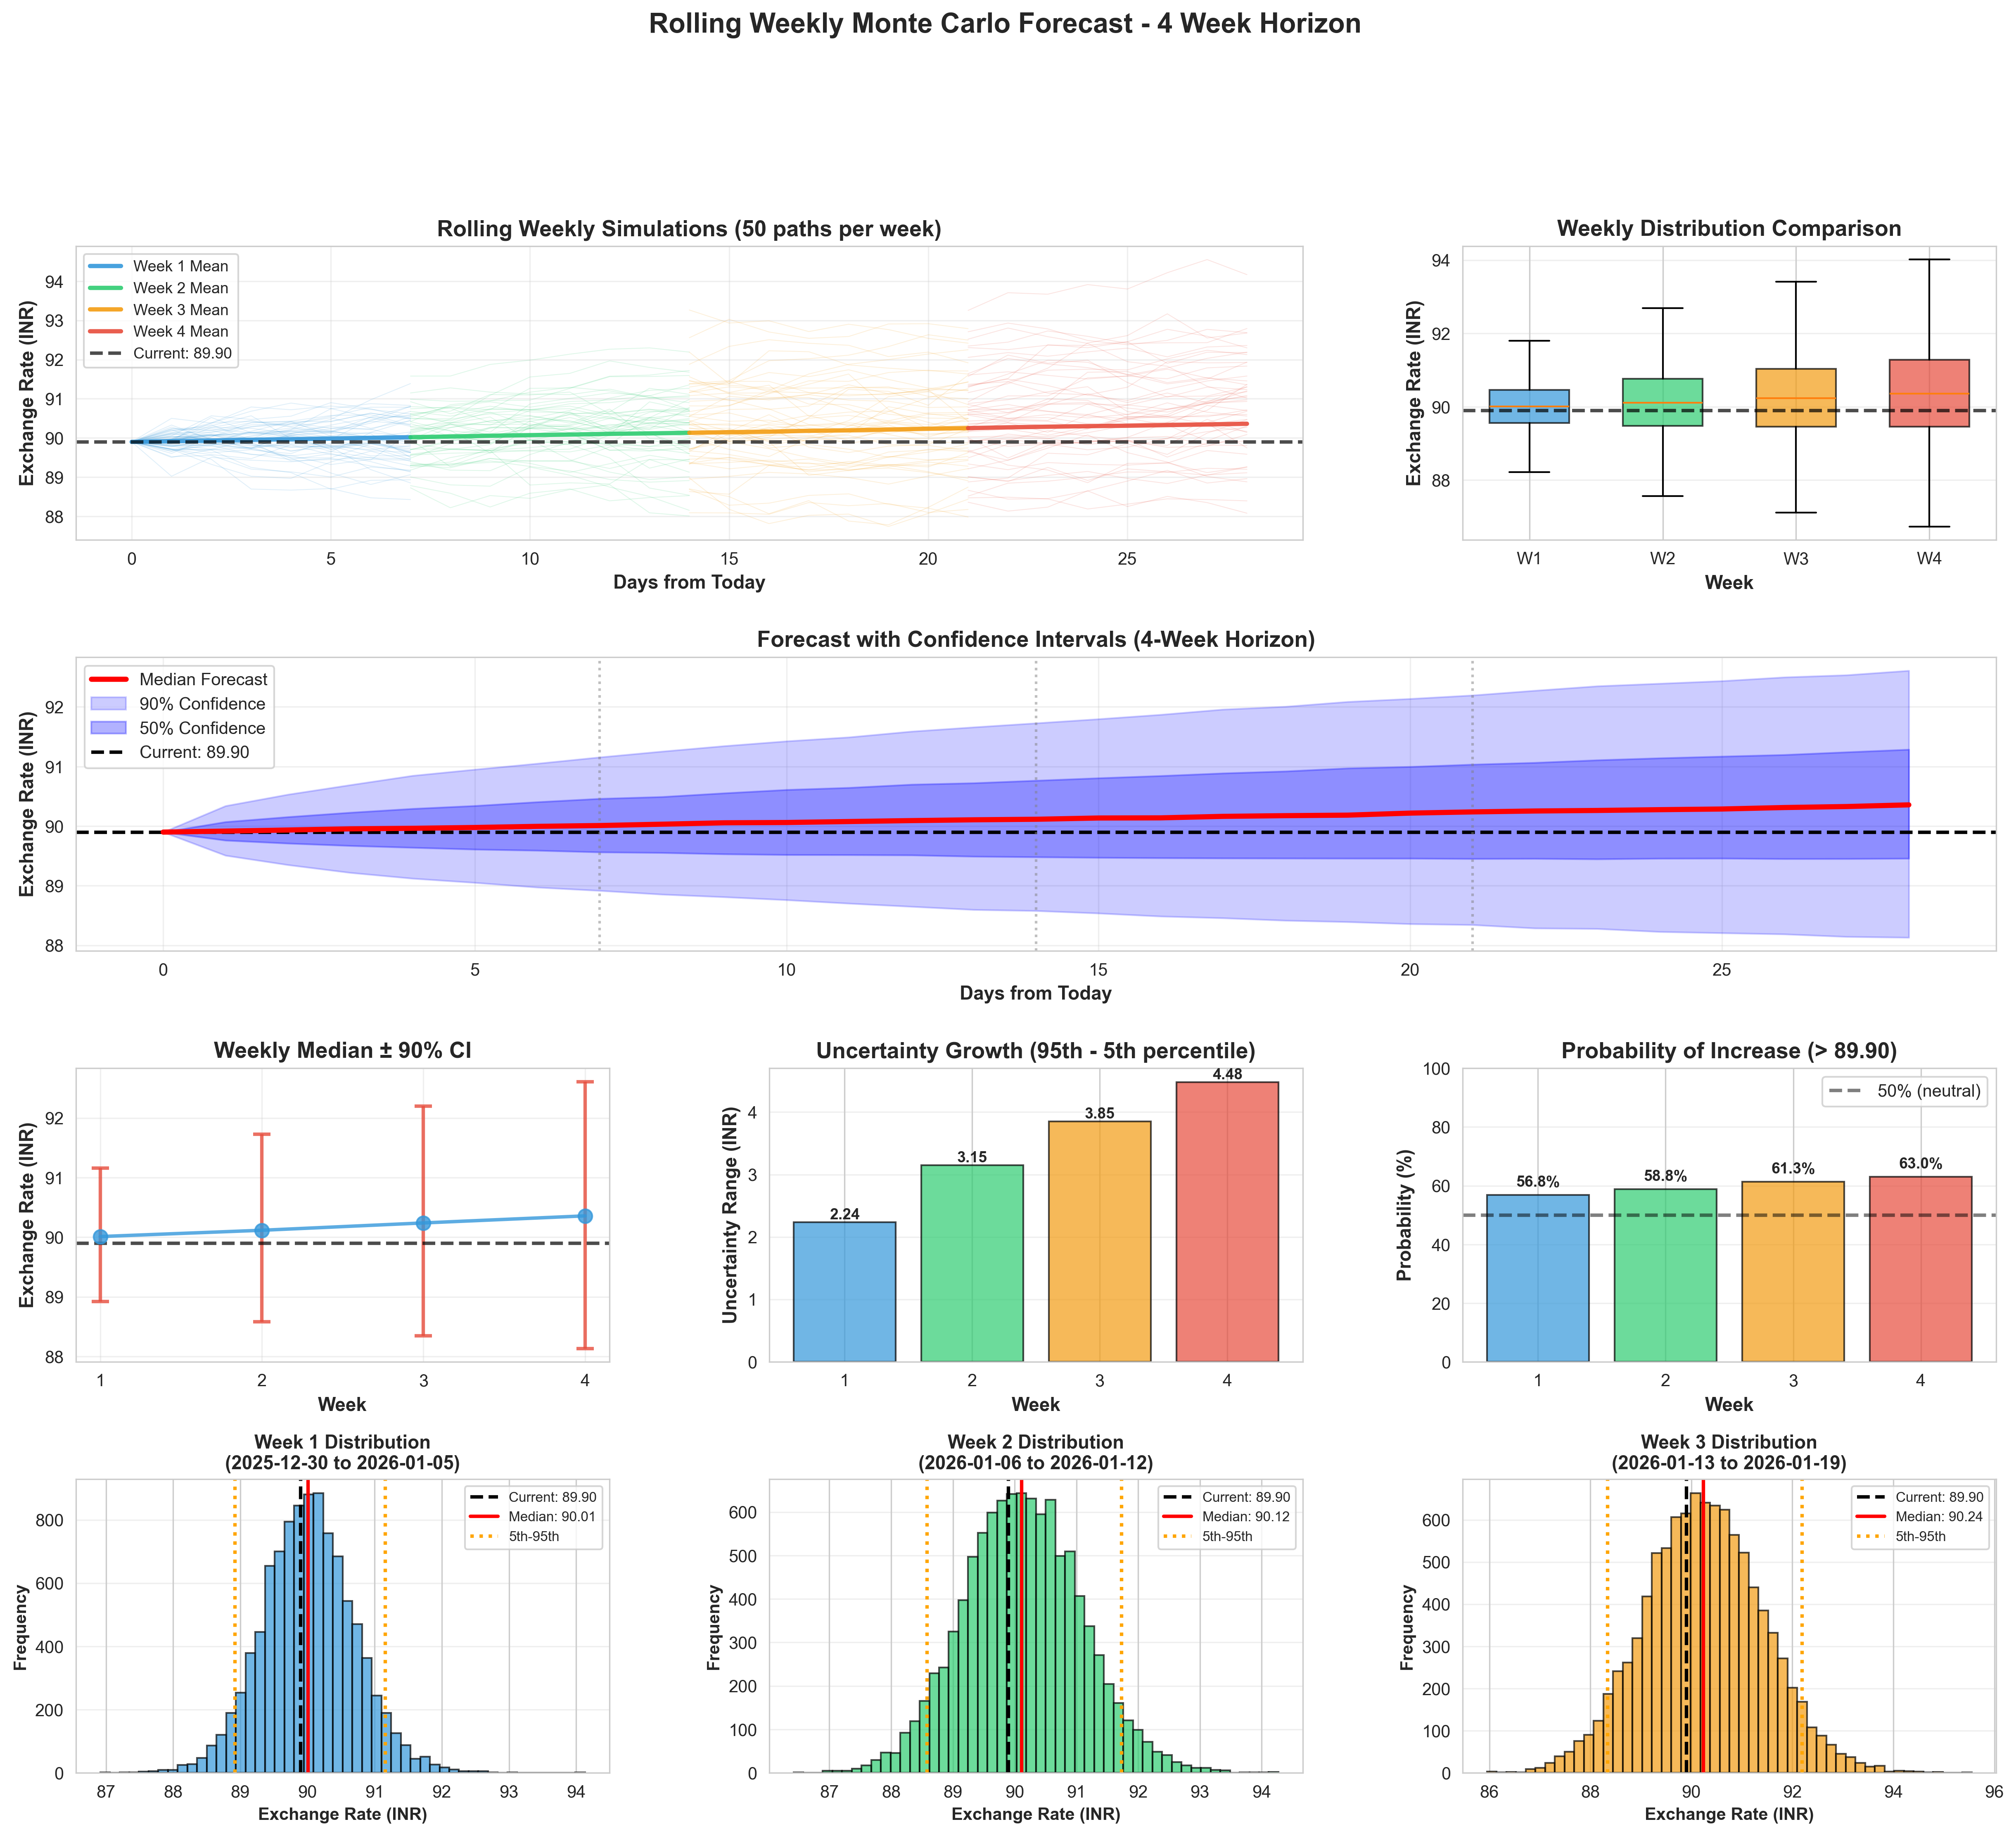
\includegraphics[width=\linewidth]{monte_carlo_weekly.png}
    \caption{Weekly rolling Monte Carlo forecast summary.}
\end{subfigure}
\caption{The quantitative middle branch of the repository ultimately favors simple trend-following plus explicit uncertainty modeling over high-capacity direct forecasters.}
\label{fig:ensemble_mc}
\end{figure*}

\subsection{Gemini V4 Improves Over V3, but Only as a Constrained Overlay}

The repository's LLM results are strongest when the LLM is treated as a bounded adjustment layer rather than a stand-alone forecaster. Using the saved per-day summary files, Table~\ref{tab:gemini_results} compares V3 and V4 under a sign-of-change directional evaluation.

\begin{table}[t]
\centering
\small
\caption{Gemini V3/V4 comparison from saved daily summary files.}
\label{tab:gemini_results}
\begin{tabular}{lcccc}
\toprule
\textbf{System} & \textbf{Days} & \textbf{Mean Abs.\ Error (\%)} & \textbf{Direction Acc.} & \textbf{Stat / LLM Weights} \\
\midrule
V3 hybrid days & 240 & 0.2741 & 61.25\% & 65--85 / 15--35 \\
V4 hybrid days & 240 & \textbf{0.2695} & \textbf{64.17\%} & 55--85 / 15--45 \\
V4 Jan 2026 live & 21 total & 0.3216 & 57.14\% & 62--85 / 15--38 \\
\bottomrule
\end{tabular}
\end{table}

Project presentations summarize V4 directional performance more conservatively (roughly 54--58\%) under a different scoring convention. The branch summary files nevertheless confirm the same qualitative result: V4 improves on V3, and the improvement is attributable to better prompt design and better adaptive weighting rather than to more aggressive LLM control.

\begin{table}[t]
\centering
\small
\caption{Selected January 2026 V4 live predictions.}
\label{tab:gemini_jan}
\begin{tabular}{lcccc}
\toprule
\textbf{Date} & \textbf{Prediction} & \textbf{Actual} & \textbf{Error (\%)} & \textbf{Consensus} \\
\midrule
2026-01-02 & 89.9981 & 89.9619 & +0.0402 & Warmup \\
2026-01-16 & 90.4564 & 90.3616 & +0.1049 & 100\% higher \\
2026-01-29 & 92.0165 & 92.0408 & $-0.0265$ & 100\% higher \\
2026-01-30 & 91.8205 & 91.7819 & +0.0421 & 83.5\% higher \\
\bottomrule
\end{tabular}
\end{table}

\begin{figure*}[t]
\centering
\begin{subfigure}[t]{0.48\textwidth}
    \centering
    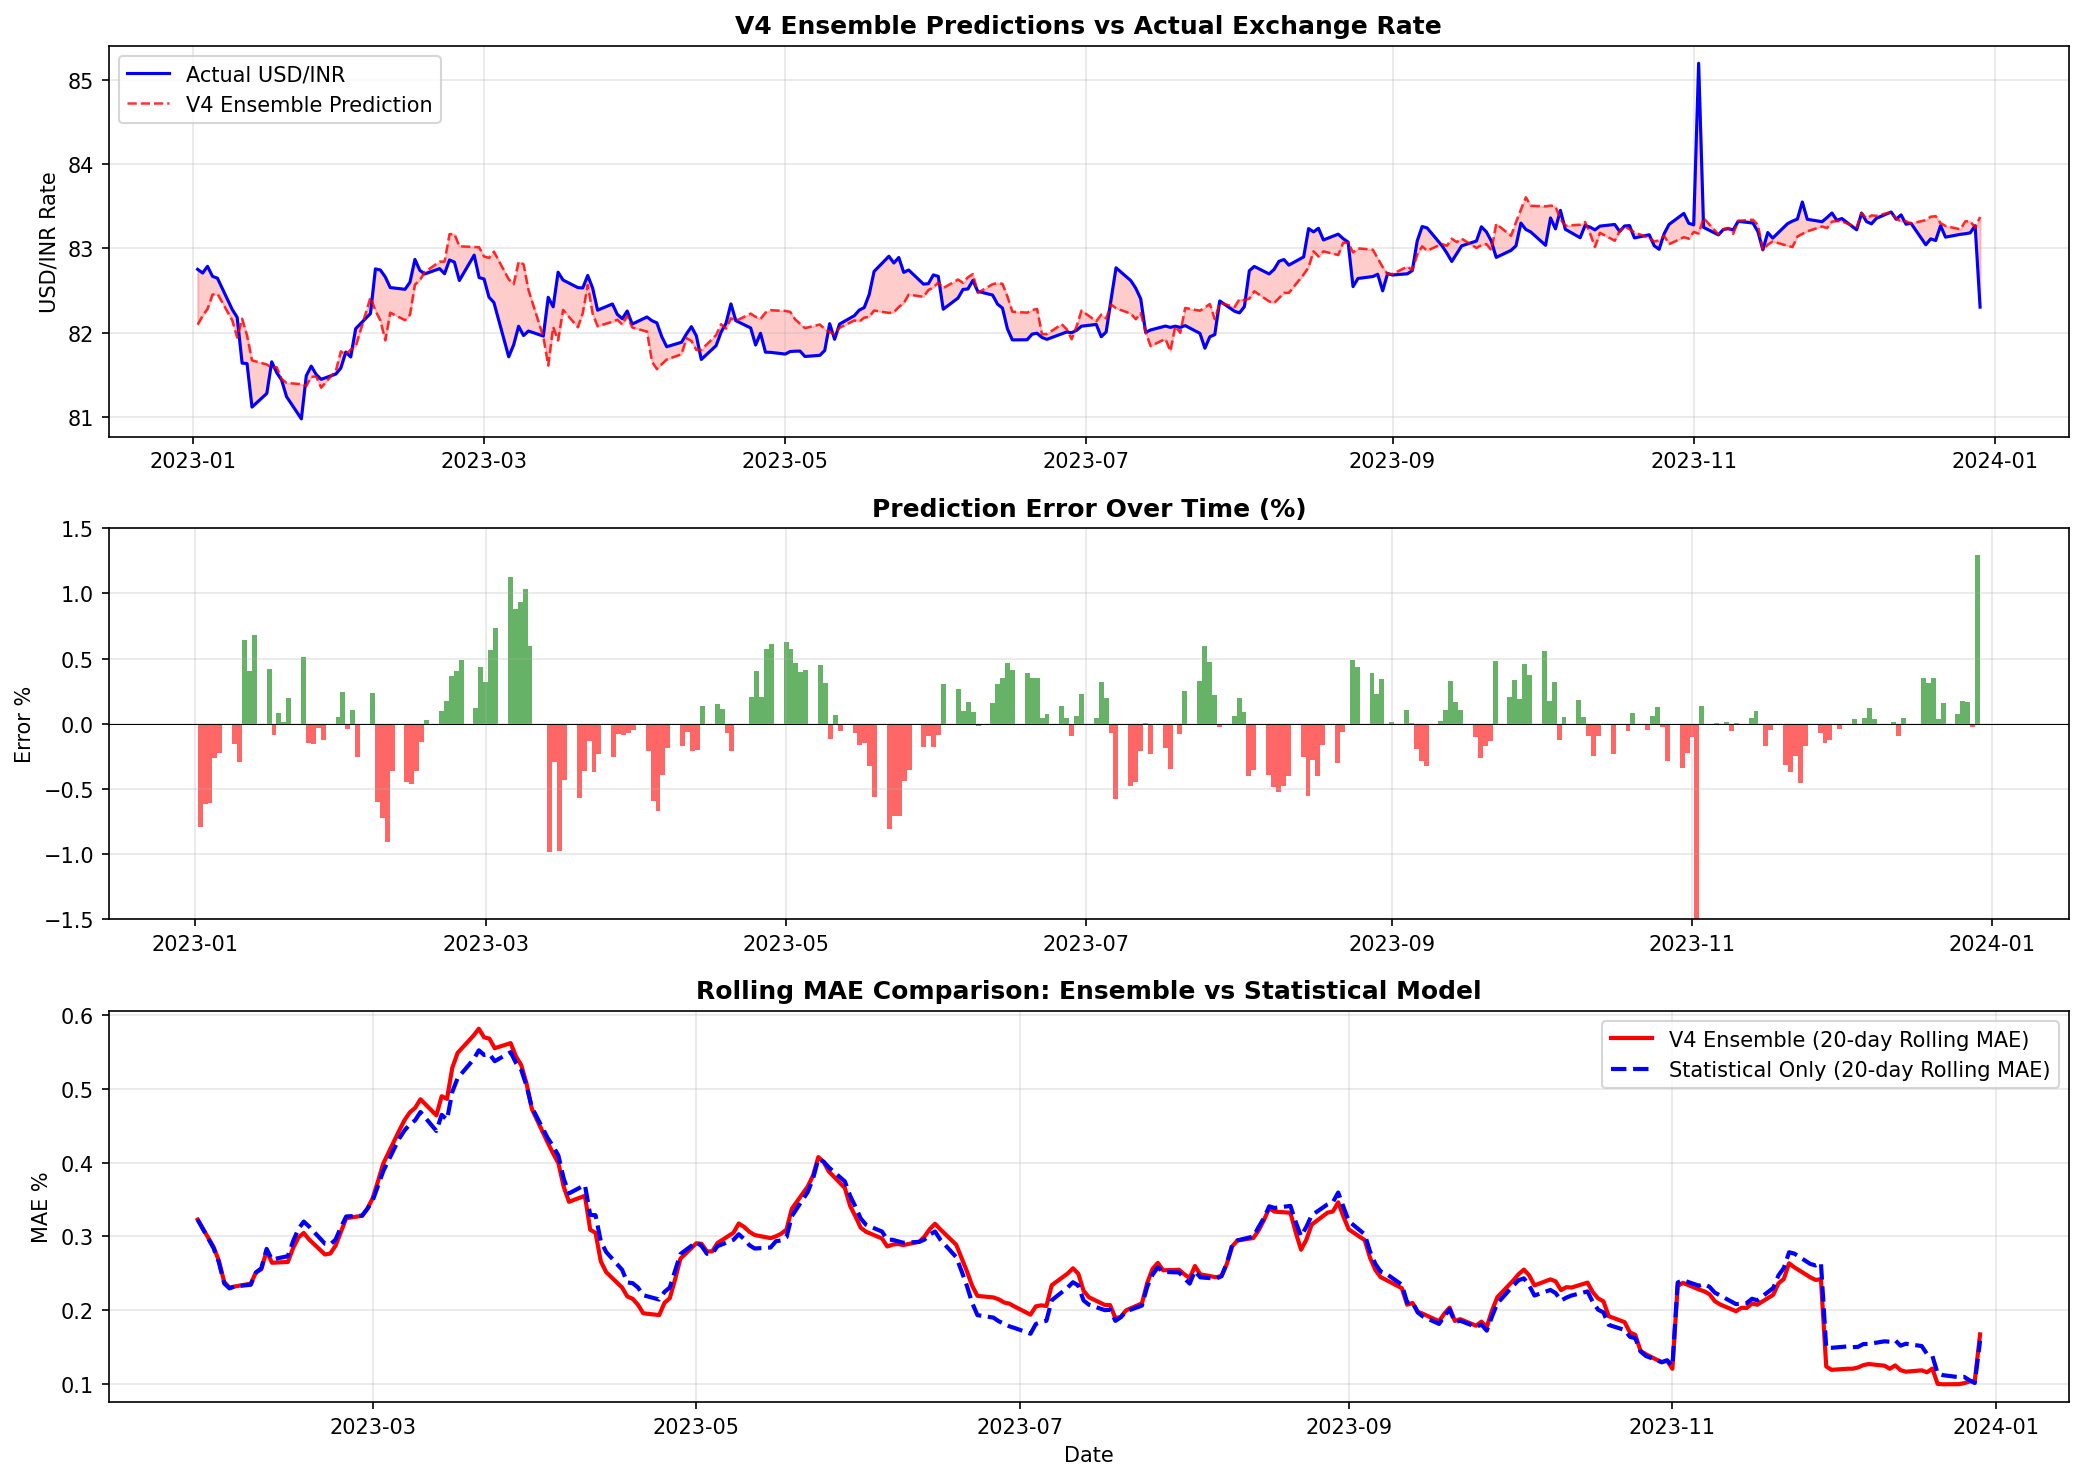
\includegraphics[width=\linewidth]{gemini_v4_comparison.png}
    \caption{Historical V4 comparison plot.}
\end{subfigure}
\hfill
\begin{subfigure}[t]{0.48\textwidth}
    \centering
    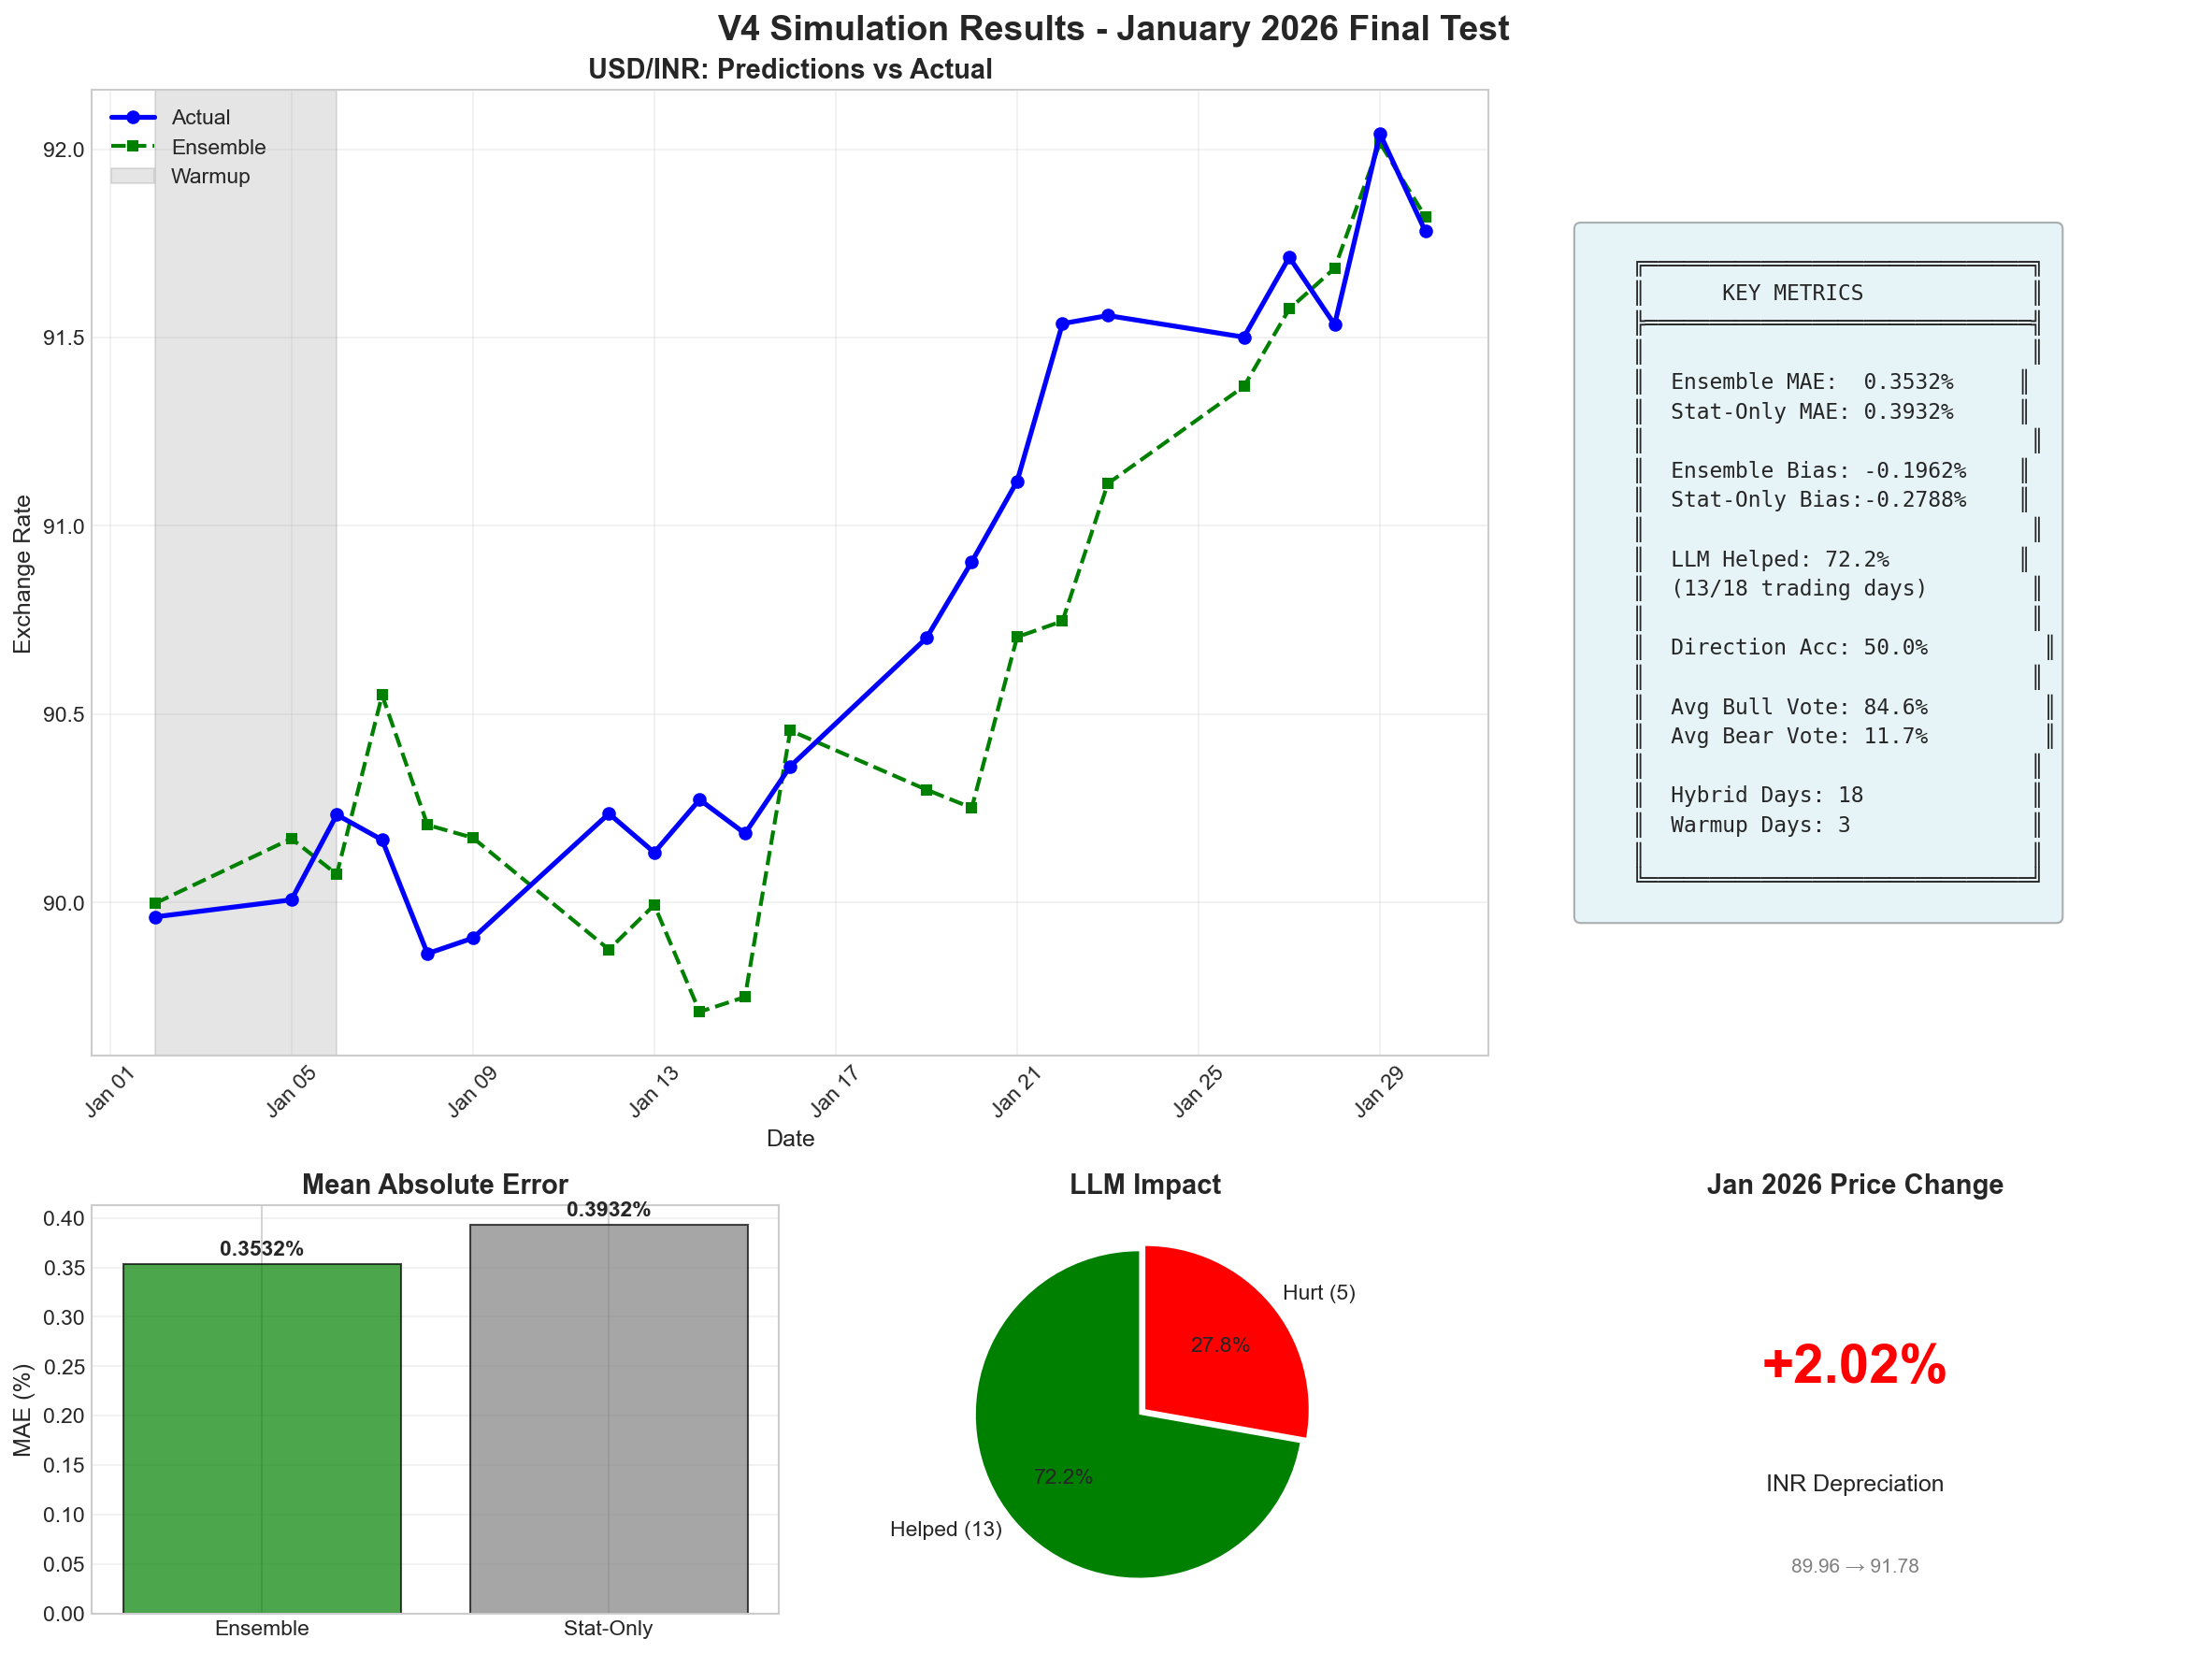
\includegraphics[width=\linewidth]{gemini_v4_jan_dashboard.png}
    \caption{January 2026 dashboard.}
\end{subfigure}
\caption{Gemini V4 adds value only when it is constrained by statistical anchors, explicit confidence logic, and persona diversification.}
\label{fig:gemini_results_fig}
\end{figure*}

\subsection{\texttt{final phase}: Market Memory Beats Heavier Blends in the 100-Day Backtest}

The most current hybrid branch produces one of the paper's most surprising results. On the 100-day walk-forward backtest, the best model is not the full feature stack, nor the rule personas, nor the standalone Gemini run. It is the \texttt{memory\_only\_no\_personas} ablation.

\begin{table}[t]
\centering
\small
\caption{\texttt{final phase} 100-day backtest ablations.}
\label{tab:finalphase_100}
\begin{tabular}{lcccc}
\toprule
\textbf{Experiment} & \textbf{MAE Price} & \textbf{RMSE Price} & \textbf{MAE Return} & \textbf{Dir.\ Acc.} \\
\midrule
memory\_only\_no\_personas & \textbf{0.2421} & \textbf{0.3290} & \textbf{0.002718} & \textbf{0.61} \\
stat\_ml\_no\_gdelt & 0.2473 & 0.3359 & 0.002779 & 0.49 \\
rule\_personas & 0.2901 & 0.4182 & 0.003260 & 0.58 \\
stat\_ml\_full & 0.3005 & 0.4361 & 0.003377 & 0.58 \\
stat\_ml\_no\_macro & 0.3524 & 0.5507 & 0.003955 & 0.58 \\
\bottomrule
\end{tabular}
\end{table}

This result suggests that, once immediate-price anchoring is removed, a compact shared-state representation can outperform a larger kitchen-sink feature stack. It also implies that the repository's late-stage progress is not primarily about adding more raw inputs, but about learning the right latent market summary.

The 30-day LLM matrix further sharpens this result:

\begin{table*}[t]
\centering
\small
\caption{\texttt{final phase} 30-day LLM matrix and ablation comparison.}
\label{tab:finalphase_30}
\begin{tabular}{lcccc}
\toprule
\textbf{Experiment} & \textbf{MAE Price} & \textbf{RMSE Price} & \textbf{MAE Return} & \textbf{Dir.\ Acc.} \\
\midrule
stat\_ml\_no\_gdelt & \textbf{0.3188} & \textbf{0.3966} & \textbf{0.003540} & 0.5000 \\
memory\_only\_no\_personas & 0.3295 & 0.3966 & 0.003658 & \textbf{0.5667} \\
Gemini 2.5 Flash personas & 0.4433 & 0.5696 & 0.004936 & 0.5333 \\
Claude Sonnet 4 personas & 0.4439 & 0.5698 & 0.004942 & 0.5333 \\
GPT-5 Chat personas & 0.4508 & 0.5816 & 0.005019 & 0.5333 \\
rule\_personas & 0.4907 & 0.6355 & 0.005463 & 0.5333 \\
stat\_ml\_full & 0.5060 & 0.6578 & 0.005634 & 0.5333 \\
stat\_ml\_no\_macro & 0.6419 & 0.8914 & 0.007142 & 0.5000 \\
\bottomrule
\end{tabular}
\end{table*}

Here the model selection lesson is even sharper: for this short 30-day window, news-free or memory-heavy baselines beat the richer persona stacks on price MAE. The standalone 100-day Gemini 2.5 Flash backtest (\texttt{llm\_gemini\_100d}) still performs reasonably well at MAE price 0.2726 and directional accuracy 58\%, but it does not beat the memory-only baseline.

\begin{figure*}[t]
\centering
\begin{subfigure}[t]{0.48\textwidth}
    \centering
    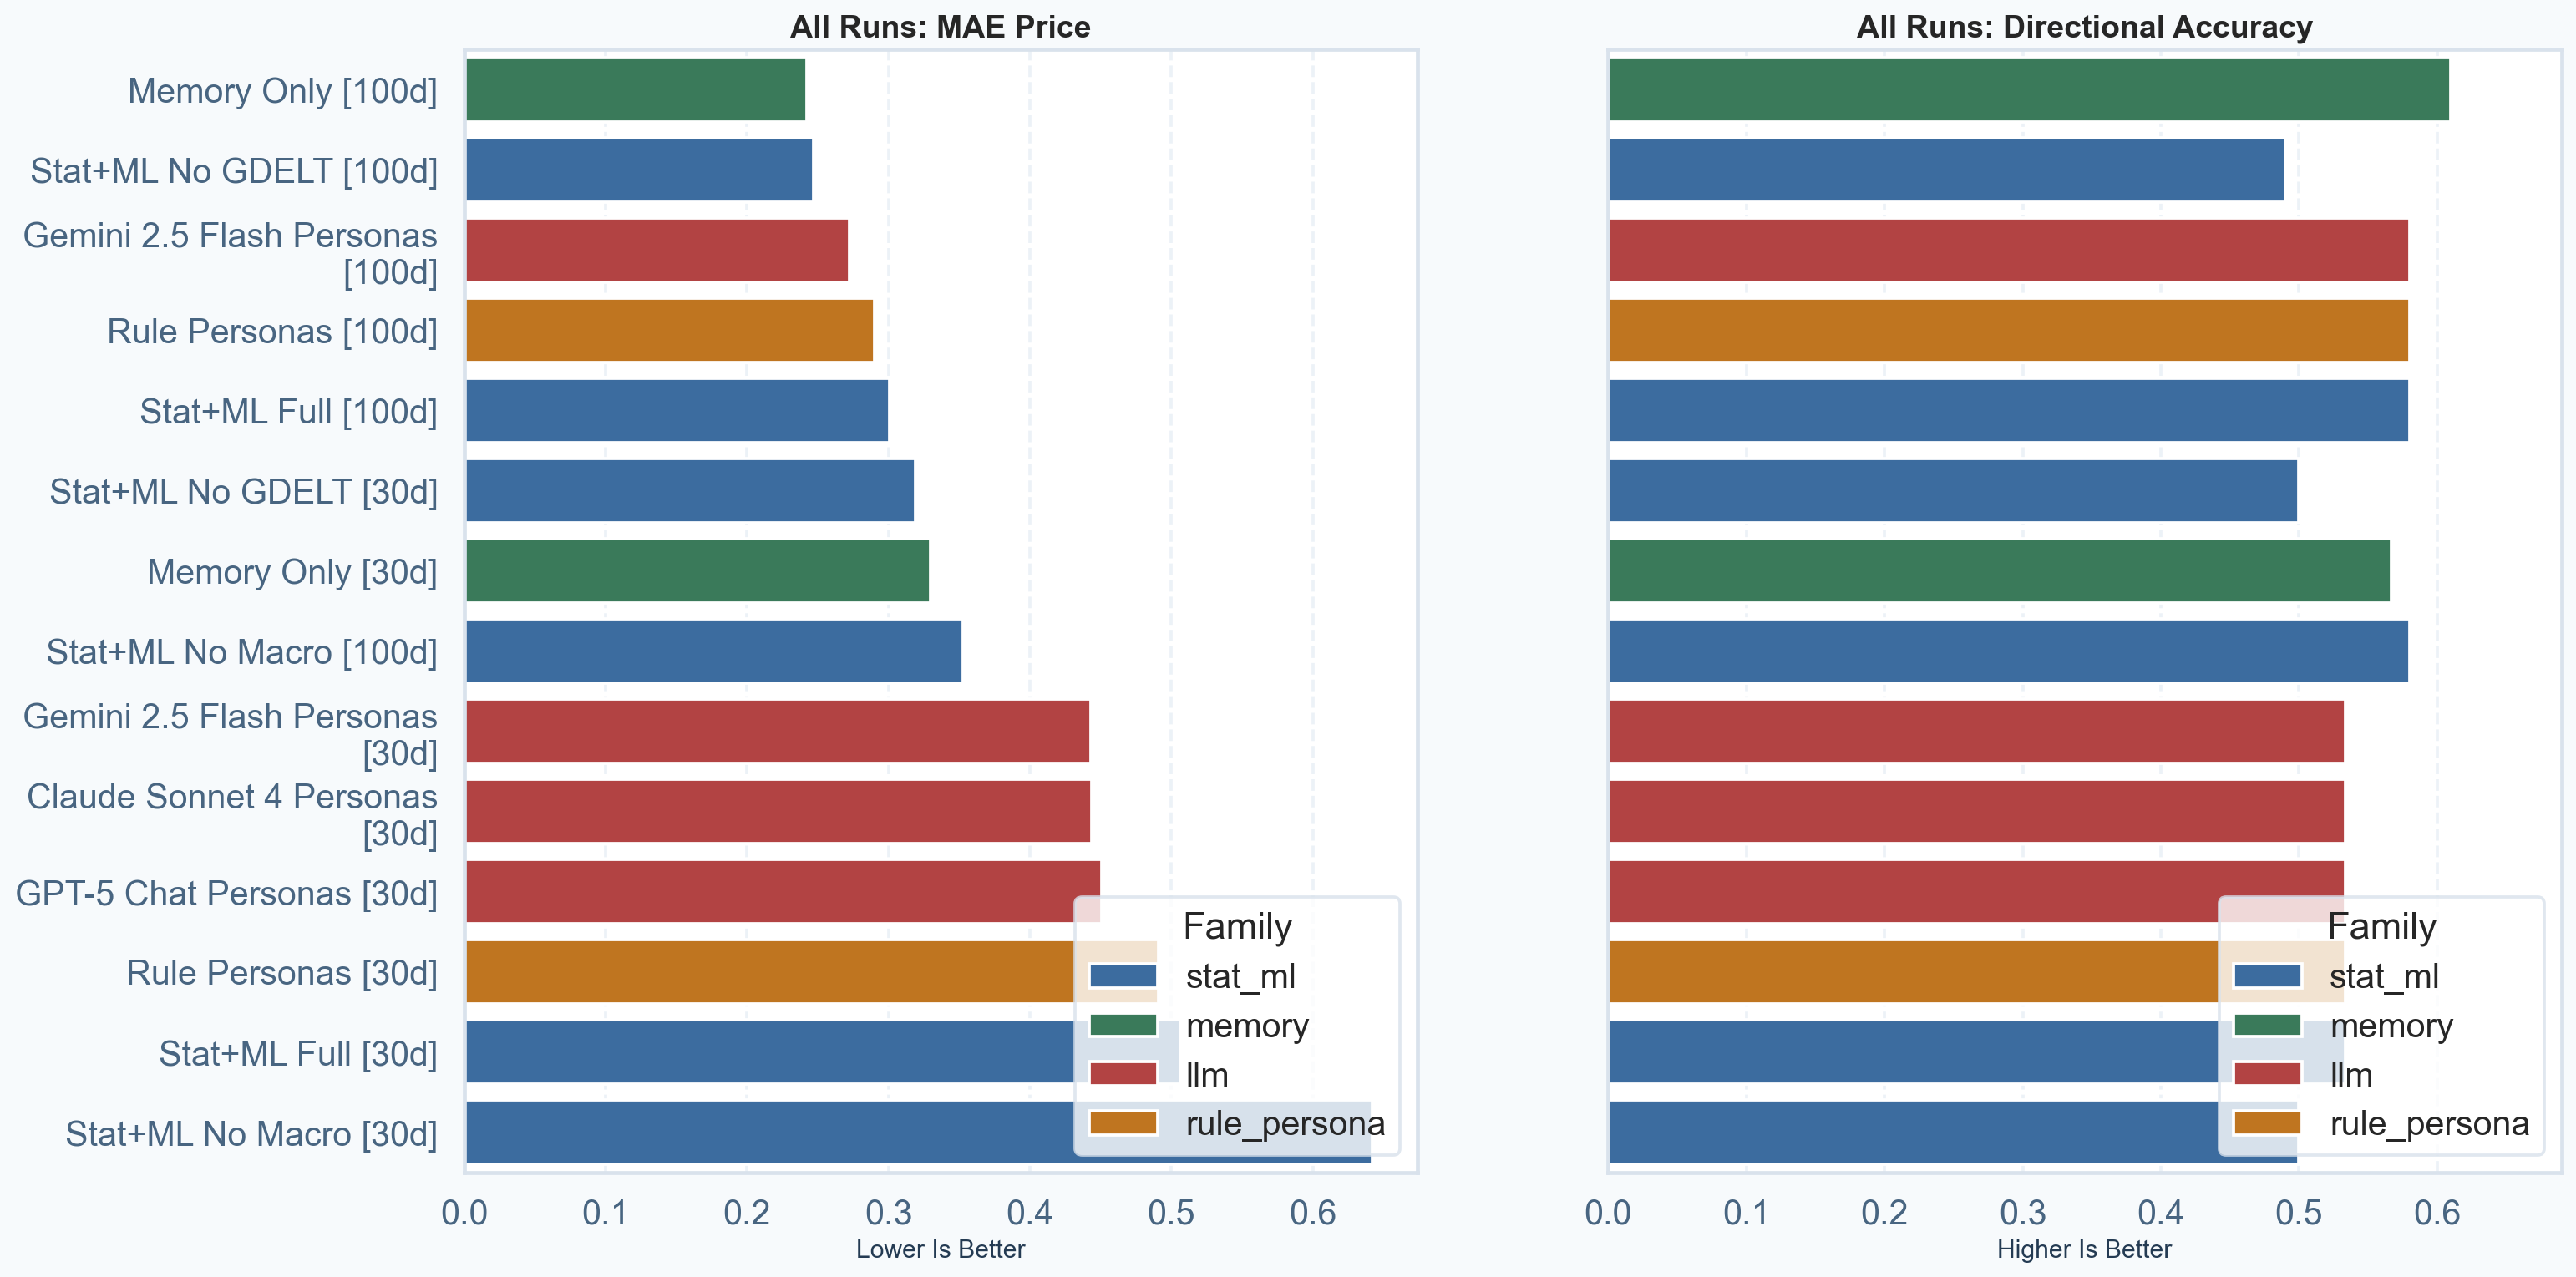
\includegraphics[width=\linewidth]{final_phase_leaderboard.png}
    \caption{Cross-run leaderboard.}
\end{subfigure}
\hfill
\begin{subfigure}[t]{0.48\textwidth}
    \centering
    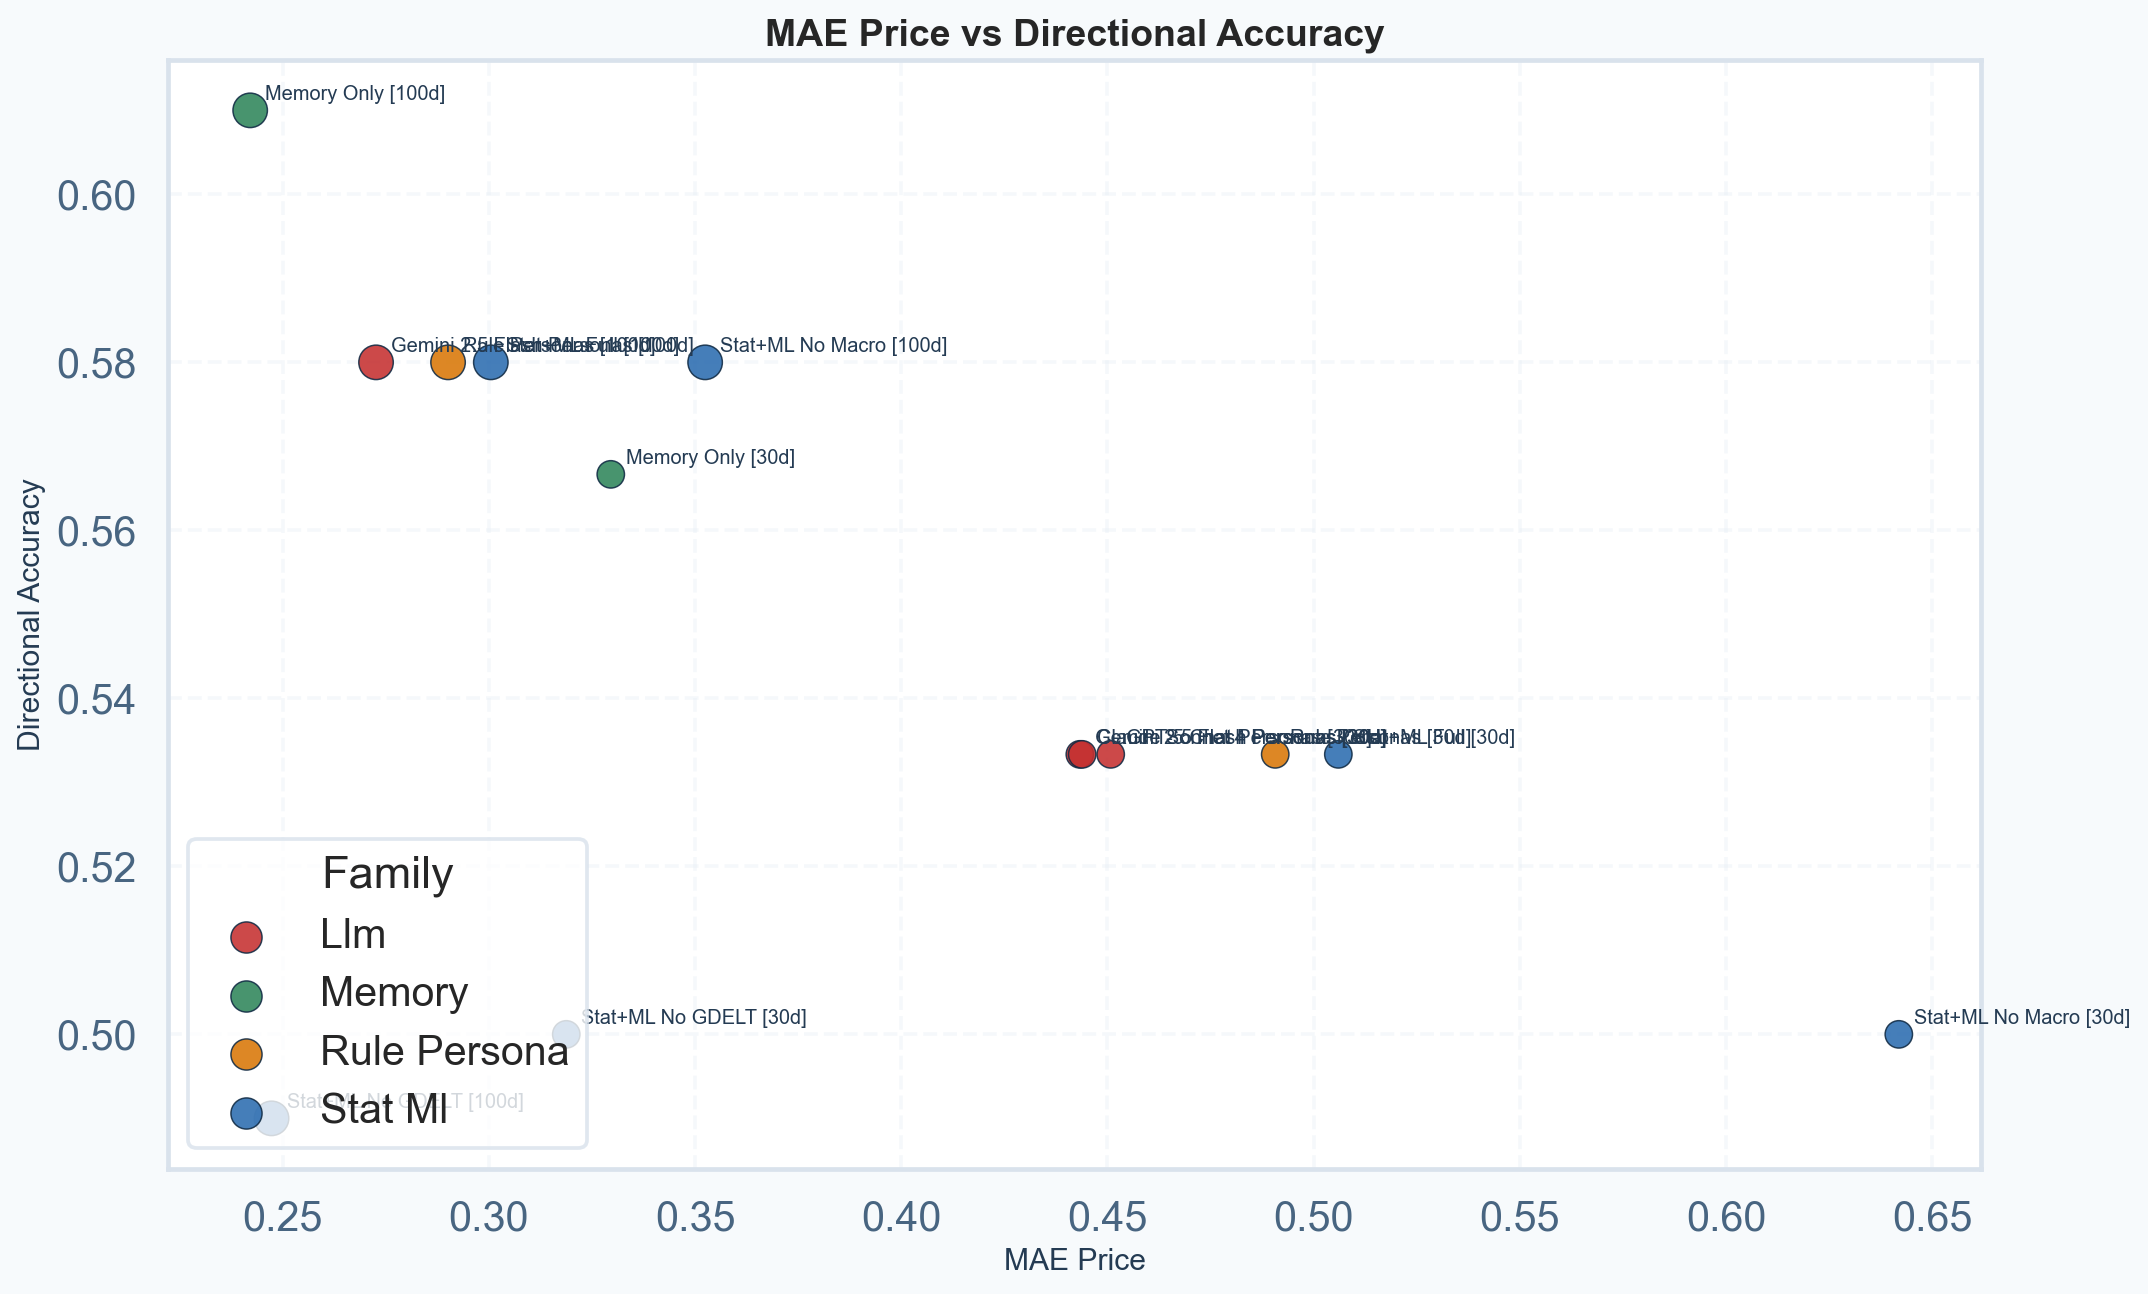
\includegraphics[width=\linewidth]{final_phase_pareto.png}
    \caption{MAE-versus-directional-accuracy Pareto view.}
\end{subfigure}
\caption{\texttt{final phase} comparison plots. The best late-stage models are not the most complex ones; compressed memory and selective feature exclusion are often stronger.}
\label{fig:finalphase}
\end{figure*}

\subsection{TEPC: Chaos and Topology Become Useful Once Timing is Made Strict}

The TEPC branch is where the repository most directly answers the ``new generation'' framing in the user's request. It is not merely a larger feature table. It is a different forecasting ontology: USD/INR as one node in a synchronized macro system.

Under the strict raw-GDELT 80-day run with a two-day response lag, the full TEPC stack is the best experiment by the branch's macro-F1-first ranking rule:

\begin{table*}[t]
\centering
\small
\caption{TEPC strict raw-GDELT 80-day ablation results.}
\label{tab:tepc_strict}
\begin{tabular}{lccccc}
\toprule
\textbf{Experiment} & \textbf{Breakout Acc.} & \textbf{Macro-F1} & \textbf{MAE Return} & \textbf{RMSE Return} & \textbf{MAE Volatility} \\
\midrule
tepc\_full & 0.7750 & \textbf{0.3370} & \textbf{0.002746} & 0.003765 & 0.000791 \\
topology\_chaos & 0.6875 & 0.3030 & 0.002991 & 0.004136 & 0.000732 \\
macro\_baseline & 0.7625 & 0.2884 & 0.002782 & \textbf{0.003755} & 0.000974 \\
chaos\_only & 0.7375 & 0.2830 & 0.003080 & 0.004088 & 0.000873 \\
topology\_only & 0.6875 & 0.2757 & 0.003352 & 0.004422 & \textbf{0.000730} \\
\bottomrule
\end{tabular}
\end{table*}

This table is revealing. Topology-only and chaos-only are individually useful but incomplete; their combination improves macro-F1 over either alone; and the full stack remains strongest overall. In other words, the branch supports the claim that topological and chaotic summaries are not gimmicks once the task is timed honestly.

The persona overlay produces a second nuance:

\begin{table}[t]
\centering
\small
\caption{TEPC strict persona-v3 overlay comparison (80-day run).}
\label{tab:tepc_persona}
\begin{tabular}{lccc}
\toprule
\textbf{Experiment} & \textbf{Breakout Acc.} & \textbf{Macro-F1} & \textbf{MAE Return} \\
\midrule
tepc\_full & 0.7750 & \textbf{0.3370} & 0.002746 \\
persona\_rule\_only & \textbf{0.8000} & 0.2963 & 0.002886 \\
tepc\_persona\_blend & 0.7875 & 0.2937 & \textbf{0.002695} \\
\bottomrule
\end{tabular}
\end{table}

The rule-persona-only system attains the highest raw breakout accuracy, but the README and run notes explain why: it acts as an abstaining range predictor in a range-heavy regime. The blended TEPC persona system, by contrast, produces the best return MAE. The branch therefore separates classifier quality, regime abstention behavior, and continuous return quality rather than collapsing them into one metric.

The livepull 100-day run adds one more important result: chaos features are the strongest classifier in that extended setup. Specifically, \texttt{chaos\_only} reaches 80\% breakout accuracy and macro-F1 0.404, while \texttt{tepc\_full} remains competitive and delivers the best return MAE at 0.003430. This is a strong indication that the chaos layer is not decorative; it becomes especially useful once richer cross-asset node feeds are available.

\begin{figure*}[t]
\centering
\begin{subfigure}[t]{0.48\textwidth}
    \centering
    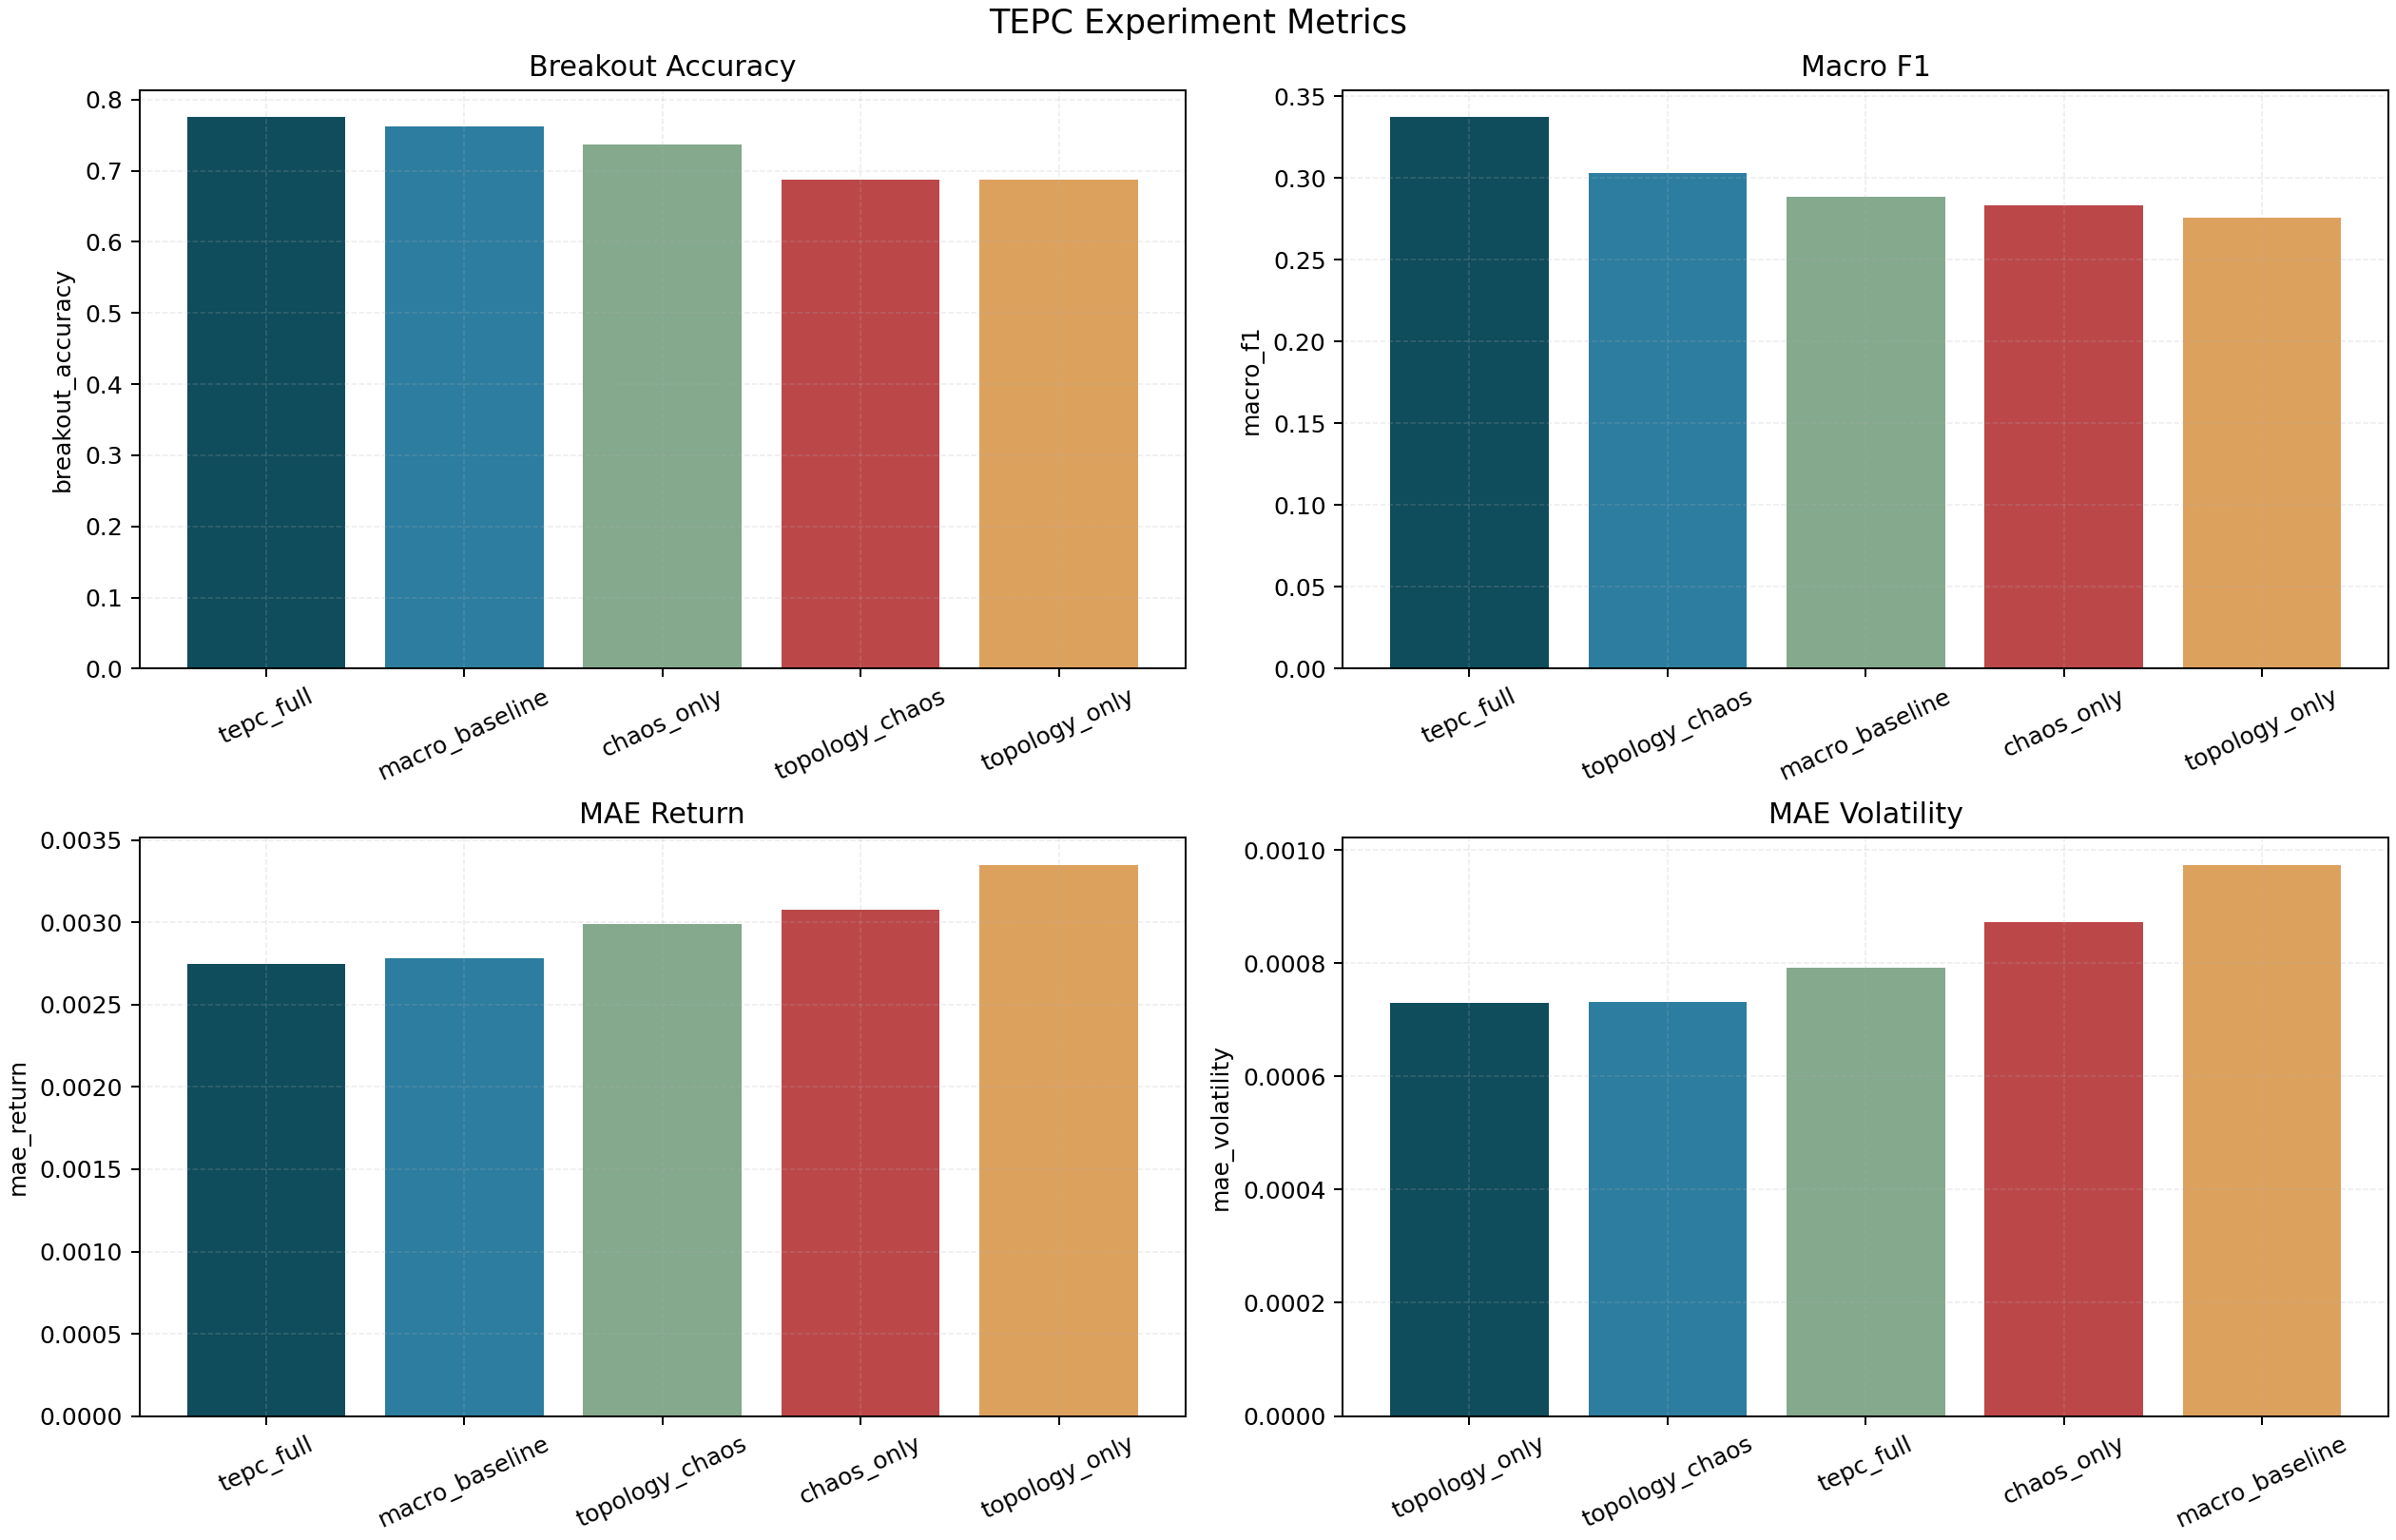
\includegraphics[width=\linewidth]{tepc_strict_metric_bars.png}
    \caption{Strict raw-GDELT TEPC metric panel.}
\end{subfigure}
\hfill
\begin{subfigure}[t]{0.48\textwidth}
    \centering
    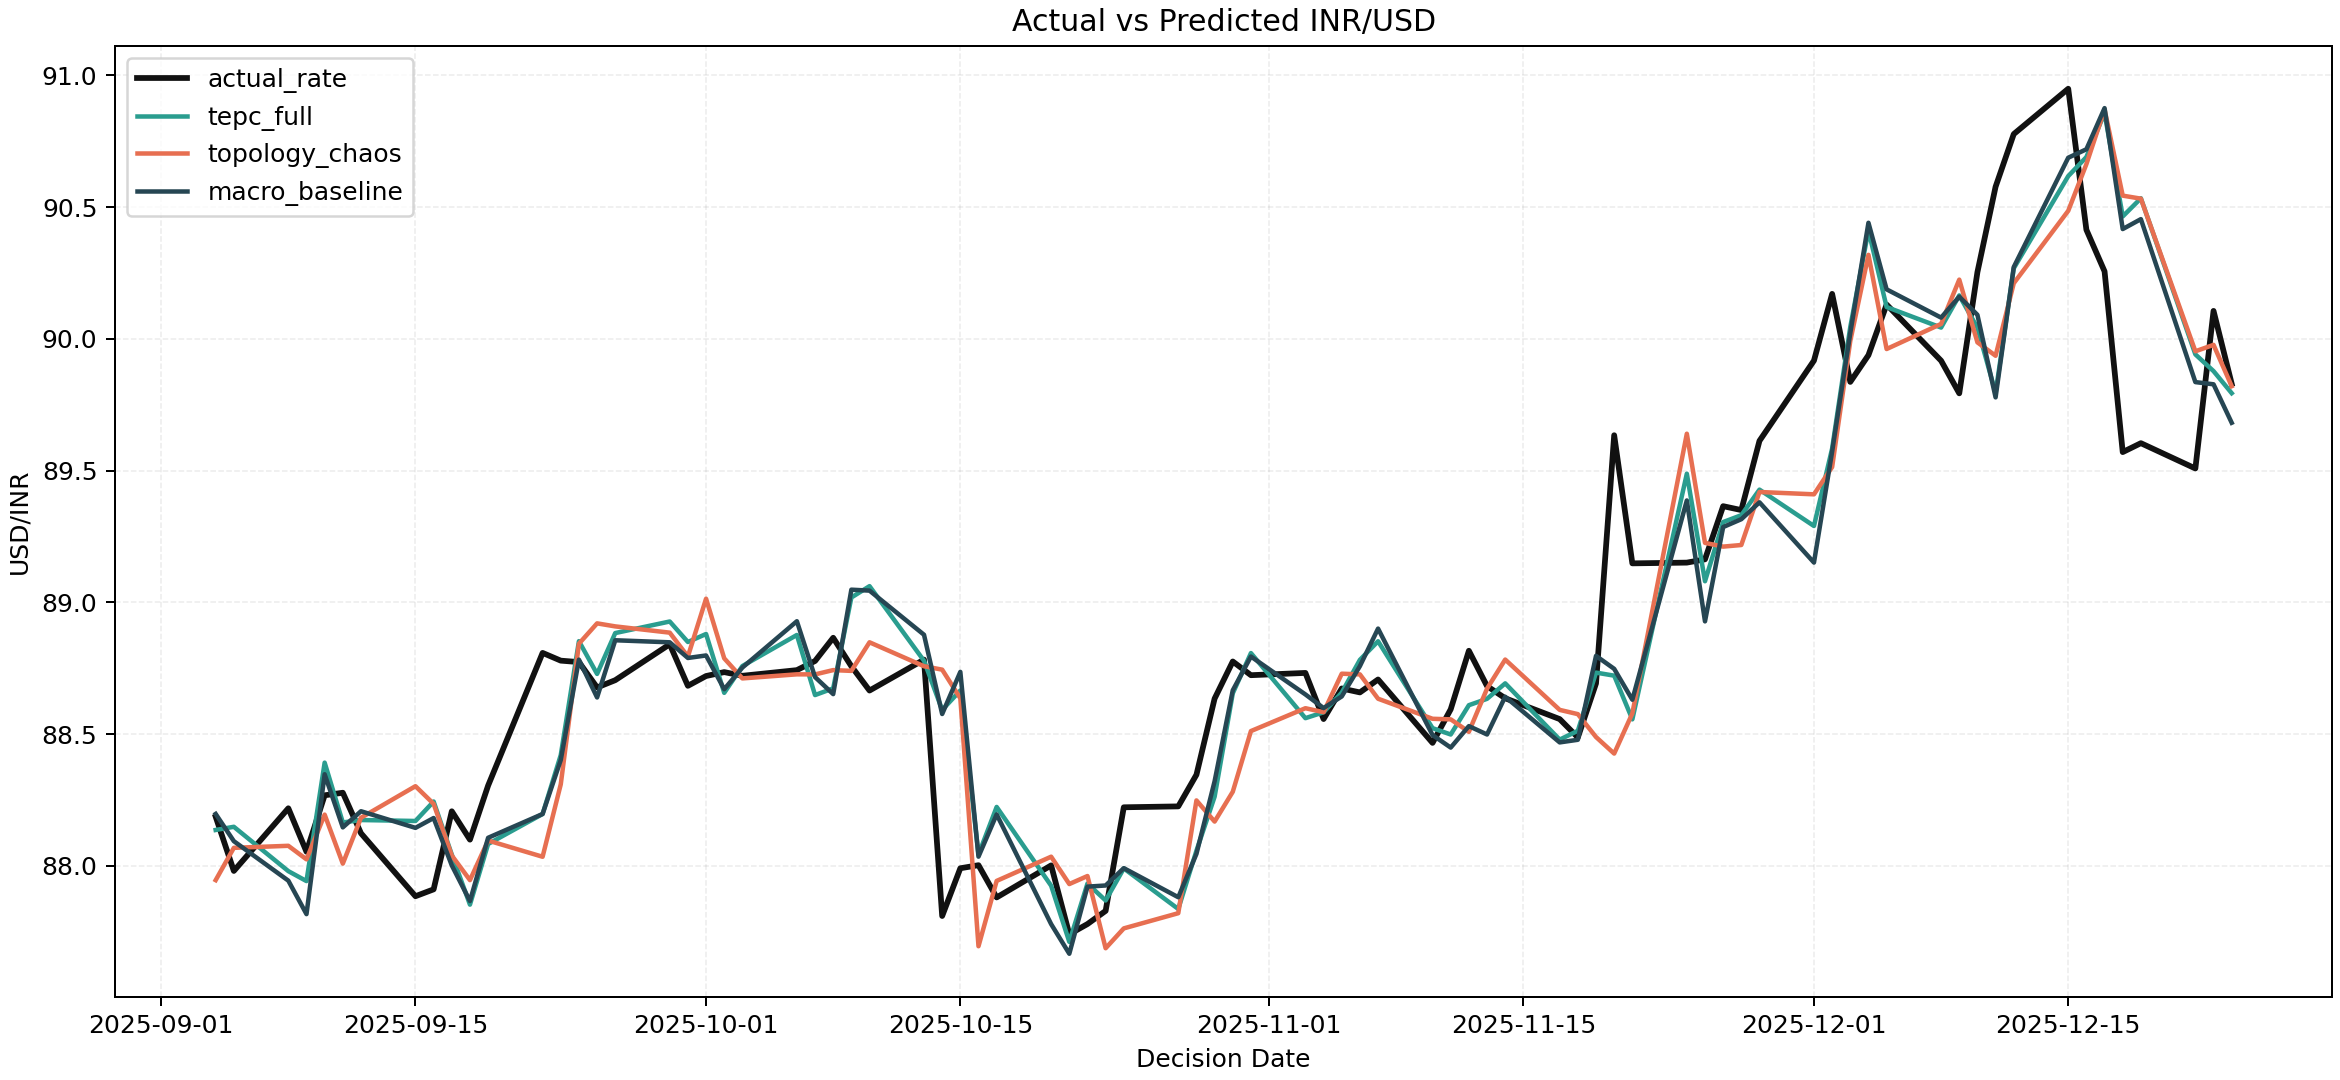
\includegraphics[width=\linewidth]{tepc_strict_predictions.png}
    \caption{Prediction overlays for the best strict TEPC experiments.}
\end{subfigure}
\caption{TEPC's strict backtest results. The topology/chaos branch becomes useful once the task explicitly prevents lag-copying and makes regime dynamics first-class.}
\label{fig:tepc}
\end{figure*}

\subsection{Cross-Branch Synthesis}

Taken together, the repository's results support five broad conclusions.

\paragraph{1. USD/INR is hostile to naive direct price prediction.}
Negative $R^2$ across ARIMA, SARIMA, LSTM, GRU, Attention, several news-augmented regressors, and the older Gemini-adjusted ensemble demonstrate that more complexity is not enough. This is exactly the sense in which the Indian FX market is ``not suitable'' for many standard models: without strong structural constraints, they mostly learn noise, persistence, or evaluation artifacts.

\paragraph{2. News is useful only after structure is imposed.}
Raw aggregate Goldstein signal is near zero against IMF$_3$, and naive political-news augmentation worsens regressors. News becomes useful after theme filtering, lag selection, event-intensity weighting, or memory/topology embedding.

\paragraph{3. Classification and state estimation beat raw regression.}
Phase C danger-day classification, \texttt{final phase} memory compression, and TEPC breakout forecasting are all more robust than exact one-step direct price regression.

\paragraph{4. LLMs help most as bounded overlays.}
Gemini V4 improves over V3, but the strongest later results come when LLMs or personas consume structured memory and are prevented from dominating the final forecast.

\paragraph{5. Topology and chaos become meaningful once timing is strict.}
TEPC's strongest results appear specifically in the strict, lagged, raw-GDELT runs where trivial lag-copying is removed. This is exactly the setting in which a network/chaos representation should matter.

\begin{table*}[t]
\centering
\small
\caption{Recommended model family by forecasting objective and horizon.}
\label{tab:recommendations}
\begin{tabular}{p{3.5cm}p{4.8cm}p{6.3cm}}
\toprule
\textbf{Objective / Horizon} & \textbf{Recommended Branch} & \textbf{Why} \\
\midrule
Danger-day / abnormal volatility flagging & Phase C XGBoost classifier & Best early branch for actionable risk alerts; precision and recall are more relevant than exact price fit. \\
Short-horizon narrative-aware next-day forecasting & Gemini V4 hybrid & Useful when a human wants a news-conditioned, persona-diversified view rather than a pure statistical forecast. \\
Walk-forward short-horizon forecasting under honest information embargo & \texttt{final phase} memory-only or no-GDELT ablations & Strongest late-stage MAE and directional results in the 100-day and 30-day backtests. \\
Breakout classification in a coupled macro regime & TEPC chaos-heavy variants and \texttt{tepc\_full} & Best repository branch for network-state and breakout interpretation under strict lagged timing. \\
Scenario analysis over weeks & Regime-switching Monte Carlo & Best when uncertainty bands and tail scenarios matter more than single-point prediction. \\
Simple practical baseline & MA\_Momentum + small GDELT ridge weight & Strongest quantitative baseline in the ultimate ensemble branch and a useful reality check against over-modeling. \\
\bottomrule
\end{tabular}
\end{table*}

% ============================================================
% 7. DISCUSSION
% ============================================================
\section{Discussion}

The repository can be read as a progressive attempt to answer a single question: \textit{what representation of the Indian FX market is stable enough to forecast?} The early answer was ``not raw price, but decomposed noise and danger-day risk.'' The middle answer was ``not a single econometric or neural architecture, but a small combination of robust quantitative priors.'' The later answer was ``not raw tabular features alone, but compact shared market state.'' TEPC adds a final answer: ``sometimes the right object is not a scalar series at all, but a synchronized macro network.''

This progression also explains why some results appear paradoxical if read superficially. It may seem strange that memory-only outperforms a richer late-stage full model, or that chaos-only is the best TEPC classifier in one setting while TEPC full is best on macro-F1 in another. But those results are coherent once USD/INR is treated as a regime-sensitive, intervention-prone market. In such a market, extra inputs help only if they are compressed correctly; otherwise they increase variance more than signal.

The same logic resolves the role of LLMs. The repository does not support the claim that LLMs should replace classical forecasting engines. It supports a narrower, more defensible claim: multi-persona LLM systems can contribute useful incremental information when they are debiased, bounded, calibrated, and supplied with structured state rather than raw price anchors.

% ============================================================
% 8. LIMITATIONS
% ============================================================
\section{Limitations}

\begin{itemize}[leftmargin=*]
    \item \textbf{Heterogeneous benchmarks.} The repository contains multiple branches with different date ranges, objectives, and metrics. This paper treats them as a research program, not a single apples-to-apples benchmark.

    \item \textbf{Documentation drift.} Some older markdown files report slightly different summary statistics from the saved CSVs. Where this occurred, the paper prioritizes direct artifact values and explicitly notes when evaluation conventions differ.

    \item \textbf{Missing requested baselines.} ARDL and DMI-style benchmarks were requested conceptually, but no reproducible saved artifacts for those methods were found in the repository snapshot. They are therefore discussed only as absent baselines, not as reported empirical results.

    \item \textbf{Limited stable windows for some branches.} Phase-B/Phase-C and several GARCH-related analyses are effectively 2025 experiments. TEPC strict raw-GDELT runs are currently tied to local raw news coverage availability.

    \item \textbf{LLM reproducibility.} The Gemini and later multi-provider persona branches depend on external model APIs and prompting behavior, which are more reproducible than free-form qualitative use but still less stable than fully local numeric pipelines.

    \item \textbf{No transaction-cost model.} The repository studies predictability, regime detection, and risk. It does not yet include execution slippage, spread costs, or treasury workflow constraints needed for deployment.
\end{itemize}

% ============================================================
% 9. CONCLUSION
% ============================================================
\section{Conclusion}

This paper documents the full repository as a single evolving research program on USD/INR forecasting. The overarching conclusion is not that one final model ``solves'' FX prediction. It is that different layers of the market are predictable with different tools. The early phases show that decomposed volatility and lagged thematic sentiment contain usable delayed structure. The GARCH and ensemble branches show that many direct price models fail, and that simple momentum plus a small amount of structured signal is often stronger than heavyweight architectures. Gemini V4 demonstrates that debiased persona-based LLM forecasting can help as a bounded overlay. The \texttt{final phase} stack shows that compressed market memory can outperform richer feature blends under honest walk-forward evaluation. TEPC finally shows that topology and chaos are not cosmetic additions; under strict lagged timing they become genuinely informative breakout and regime features.

If the repository has a single scientific message, it is this: the ``new generation'' of prediction systems for USD/INR is not one more large model. It is a layered methodology that combines decomposition, event filtering, calibrated state representation, and network-aware dynamics, while remaining skeptical of any method that wins only by copying the last price.

% ============================================================
% APPENDIX
% ============================================================
\appendix

\section{Feature and Node Inventory}
\label{app:features}

\subsection{Phase-B Feature Groups}

The early signal pipeline uses 16 daily base features:
\begin{itemize}[leftmargin=*]
    \item tone: \texttt{Tone\_Economy}, \texttt{Tone\_Conflict}, \texttt{Tone\_Policy}, \texttt{Tone\_Corporate}, \texttt{Tone\_Overall};
    \item Goldstein: \texttt{Goldstein\_Avg}, \texttt{Goldstein\_Weighted};
    \item counts: theme-level counts and total count;
    \item spikes: \texttt{Volume\_Spike}, \texttt{Volume\_Spike\_Economy}, \texttt{Volume\_Spike\_Conflict}.
\end{itemize}
Each base feature is later lagged 1--5 days, producing an 80-dimensional feature space for Phase C.

\subsection{\texttt{final phase} Feature Groups}

The saved feature builder in \texttt{final phase/final\_phase/features.py} constructs seven feature groups:
\begin{enumerate}[leftmargin=*]
    \item \textbf{technical}: multi-horizon returns, volatility, trend spread, z-score, range position, drawdown, momentum stability;
    \item \textbf{macro}: oil, gold, US10Y, DXY returns and z-scores, plus derived pressure terms;
    \item \textbf{master sentiment}: rolling India and US tone, panic, stability, mention spikes, and cross-stress variables;
    \item \textbf{goldstein}: India/US Goldstein means, differences, weighted averages, event pressure;
    \item \textbf{thematic}: rolling theme tone blocks, weighted Goldstein log, theme conflict spike, log total count;
    \item \textbf{political}: rolling political Goldstein/tone means, article and mention intensity, event spikes;
    \item \textbf{memory}: macro pressure, sentiment pressure, event heat, volatility stress, carry pressure, reversal pressure, regime score.
\end{enumerate}

\subsection{TEPC Node Universe}

The local TEPC node universe contains direct and composite nodes:
\begin{itemize}[leftmargin=*]
    \item direct market nodes: INRUSD, DXY, BRENT, GOLD, US10Y;
    \item composite sentiment/geopolitical nodes: INDIA\_SENTIMENT, US\_SENTIMENT, GOLDSTEIN\_SPREAD, GEO\_RISK, THEME\_PRESSURE;
    \item optional live or cross-FX nodes when coverage permits: EURUSD, GBPINR, USDCNH, CNHUSD, LIVE\_INDIA\_FX\_NEWS, LIVE\_USD\_MACRO\_NEWS, LIVE\_GEO\_RISK.
\end{itemize}

\section{Additional Figure Gallery}
\label{app:figures}

\begin{figure*}[p]
\centering
\begin{subfigure}[t]{0.48\textwidth}
    \centering
    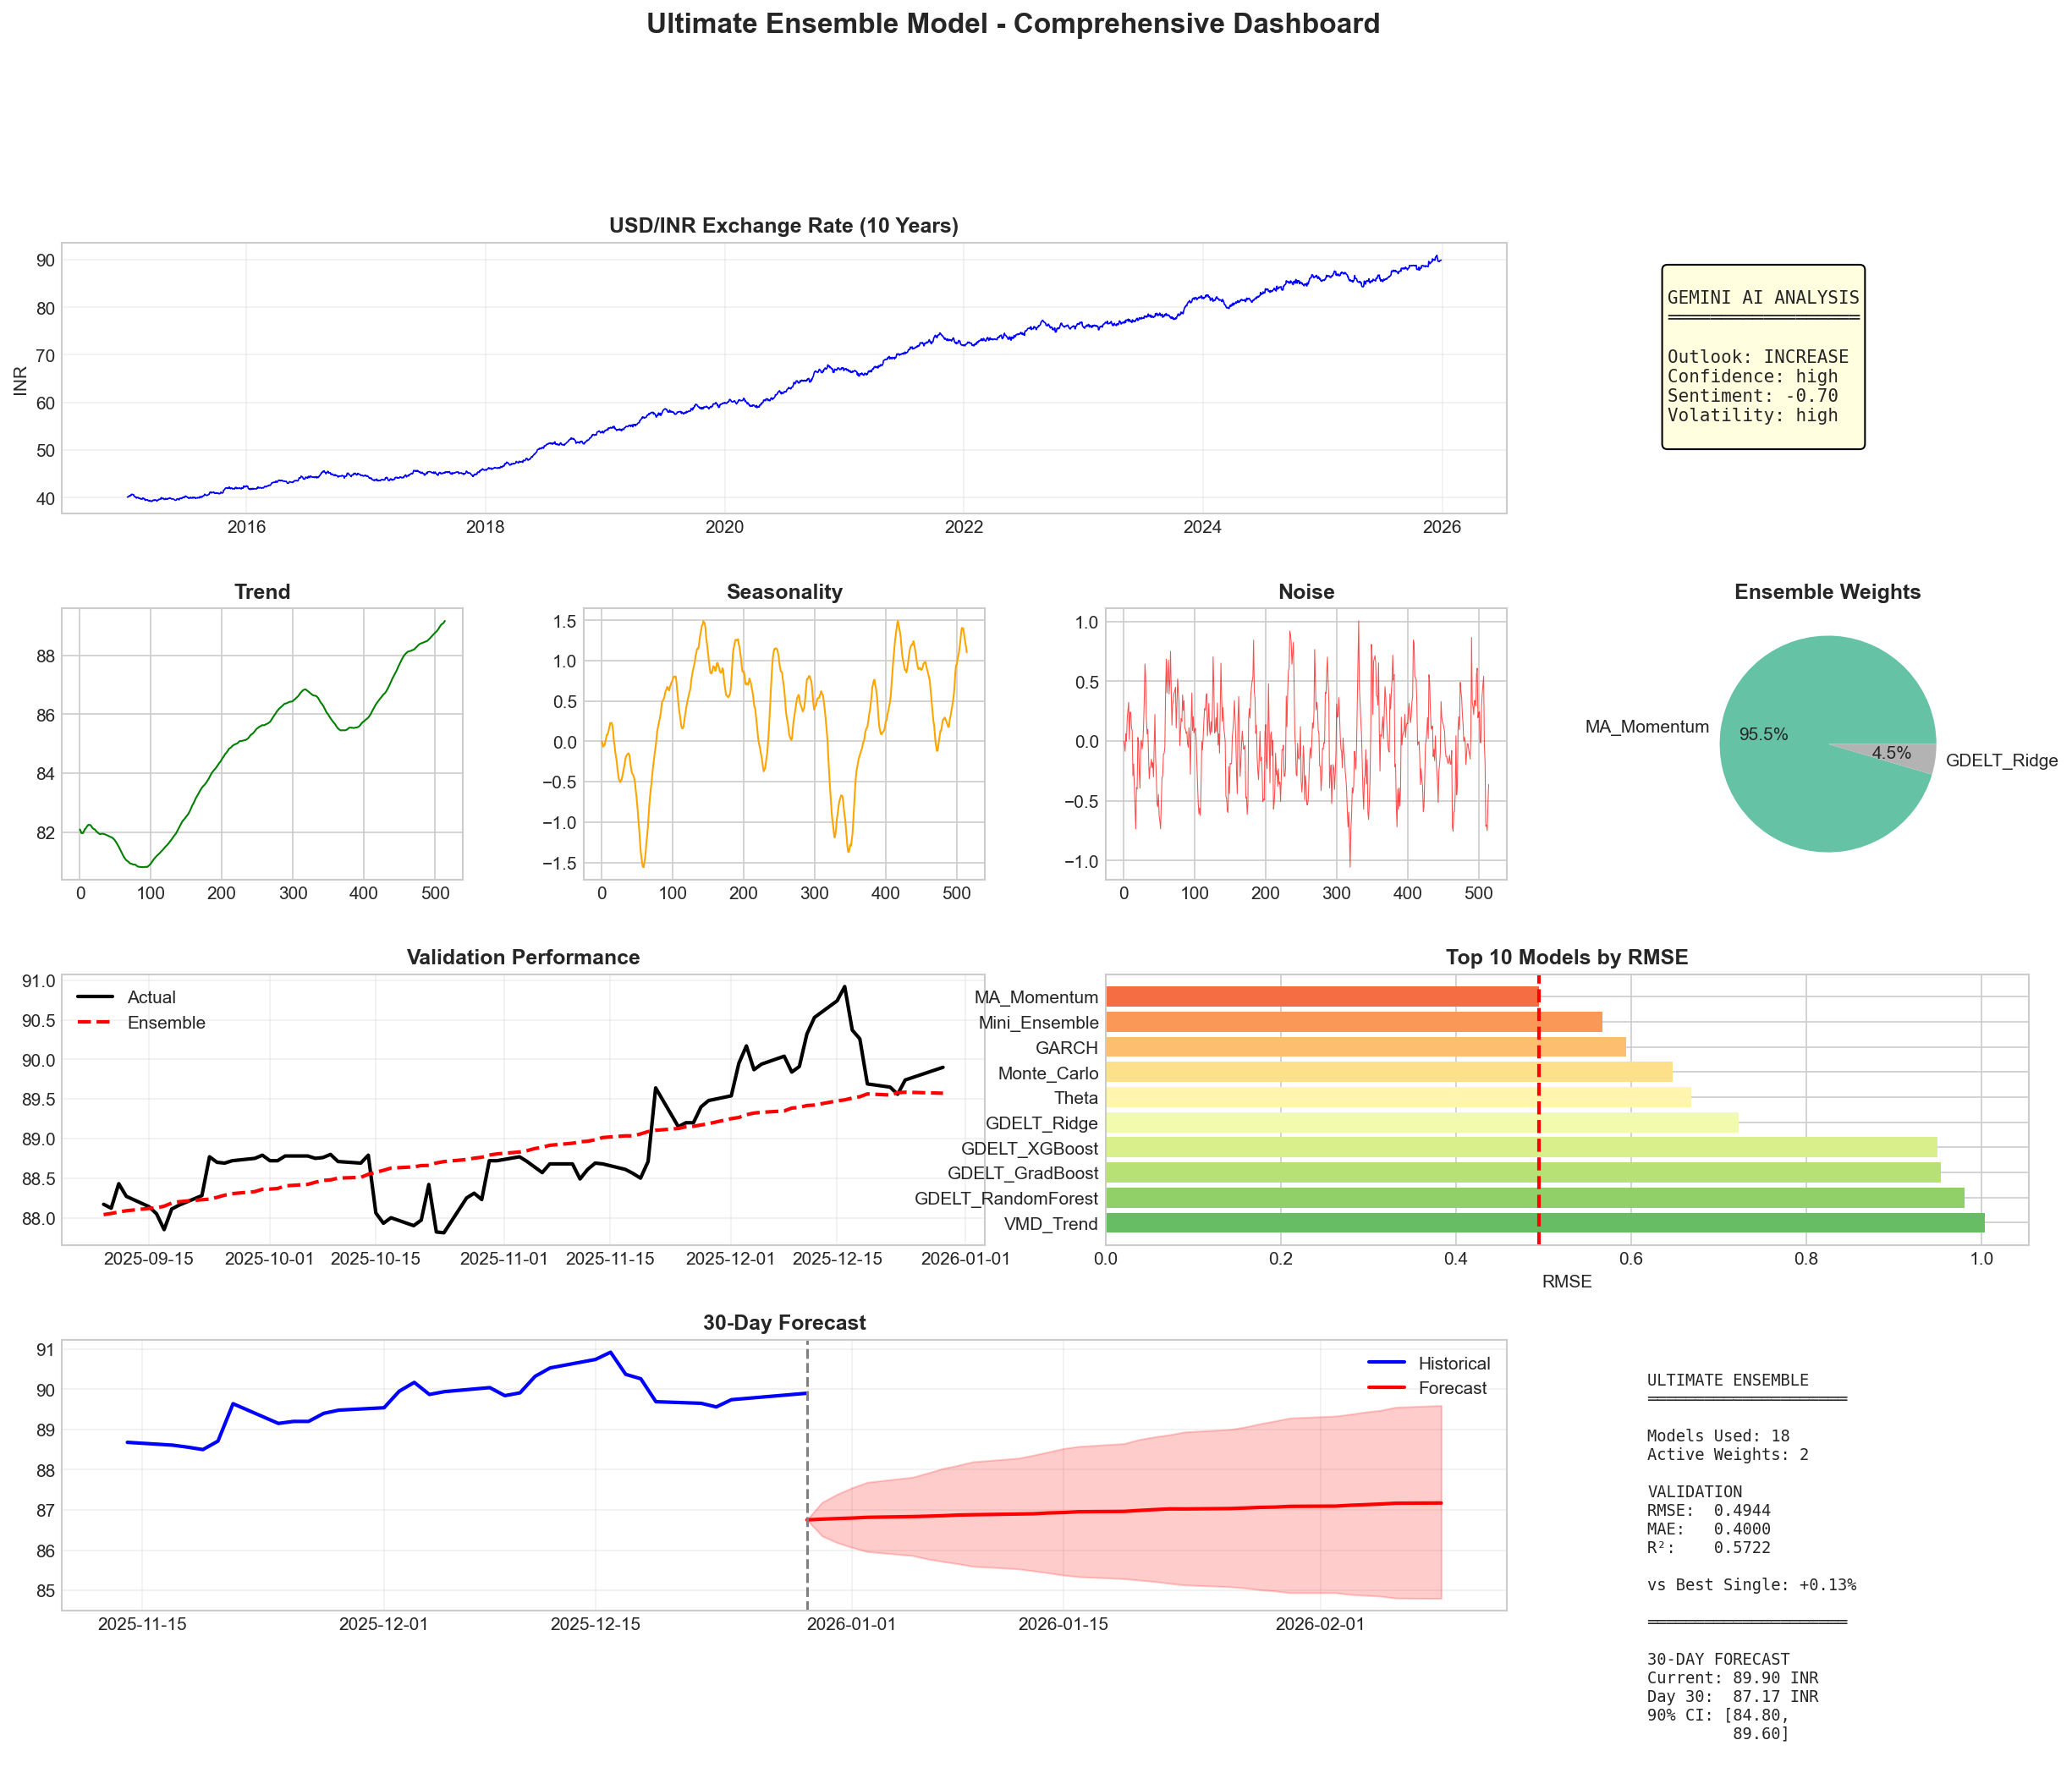
\includegraphics[width=\linewidth]{ensemble_ultimate_dashboard.png}
    \caption{Ultimate ensemble dashboard.}
\end{subfigure}
\hfill
\begin{subfigure}[t]{0.48\textwidth}
    \centering
    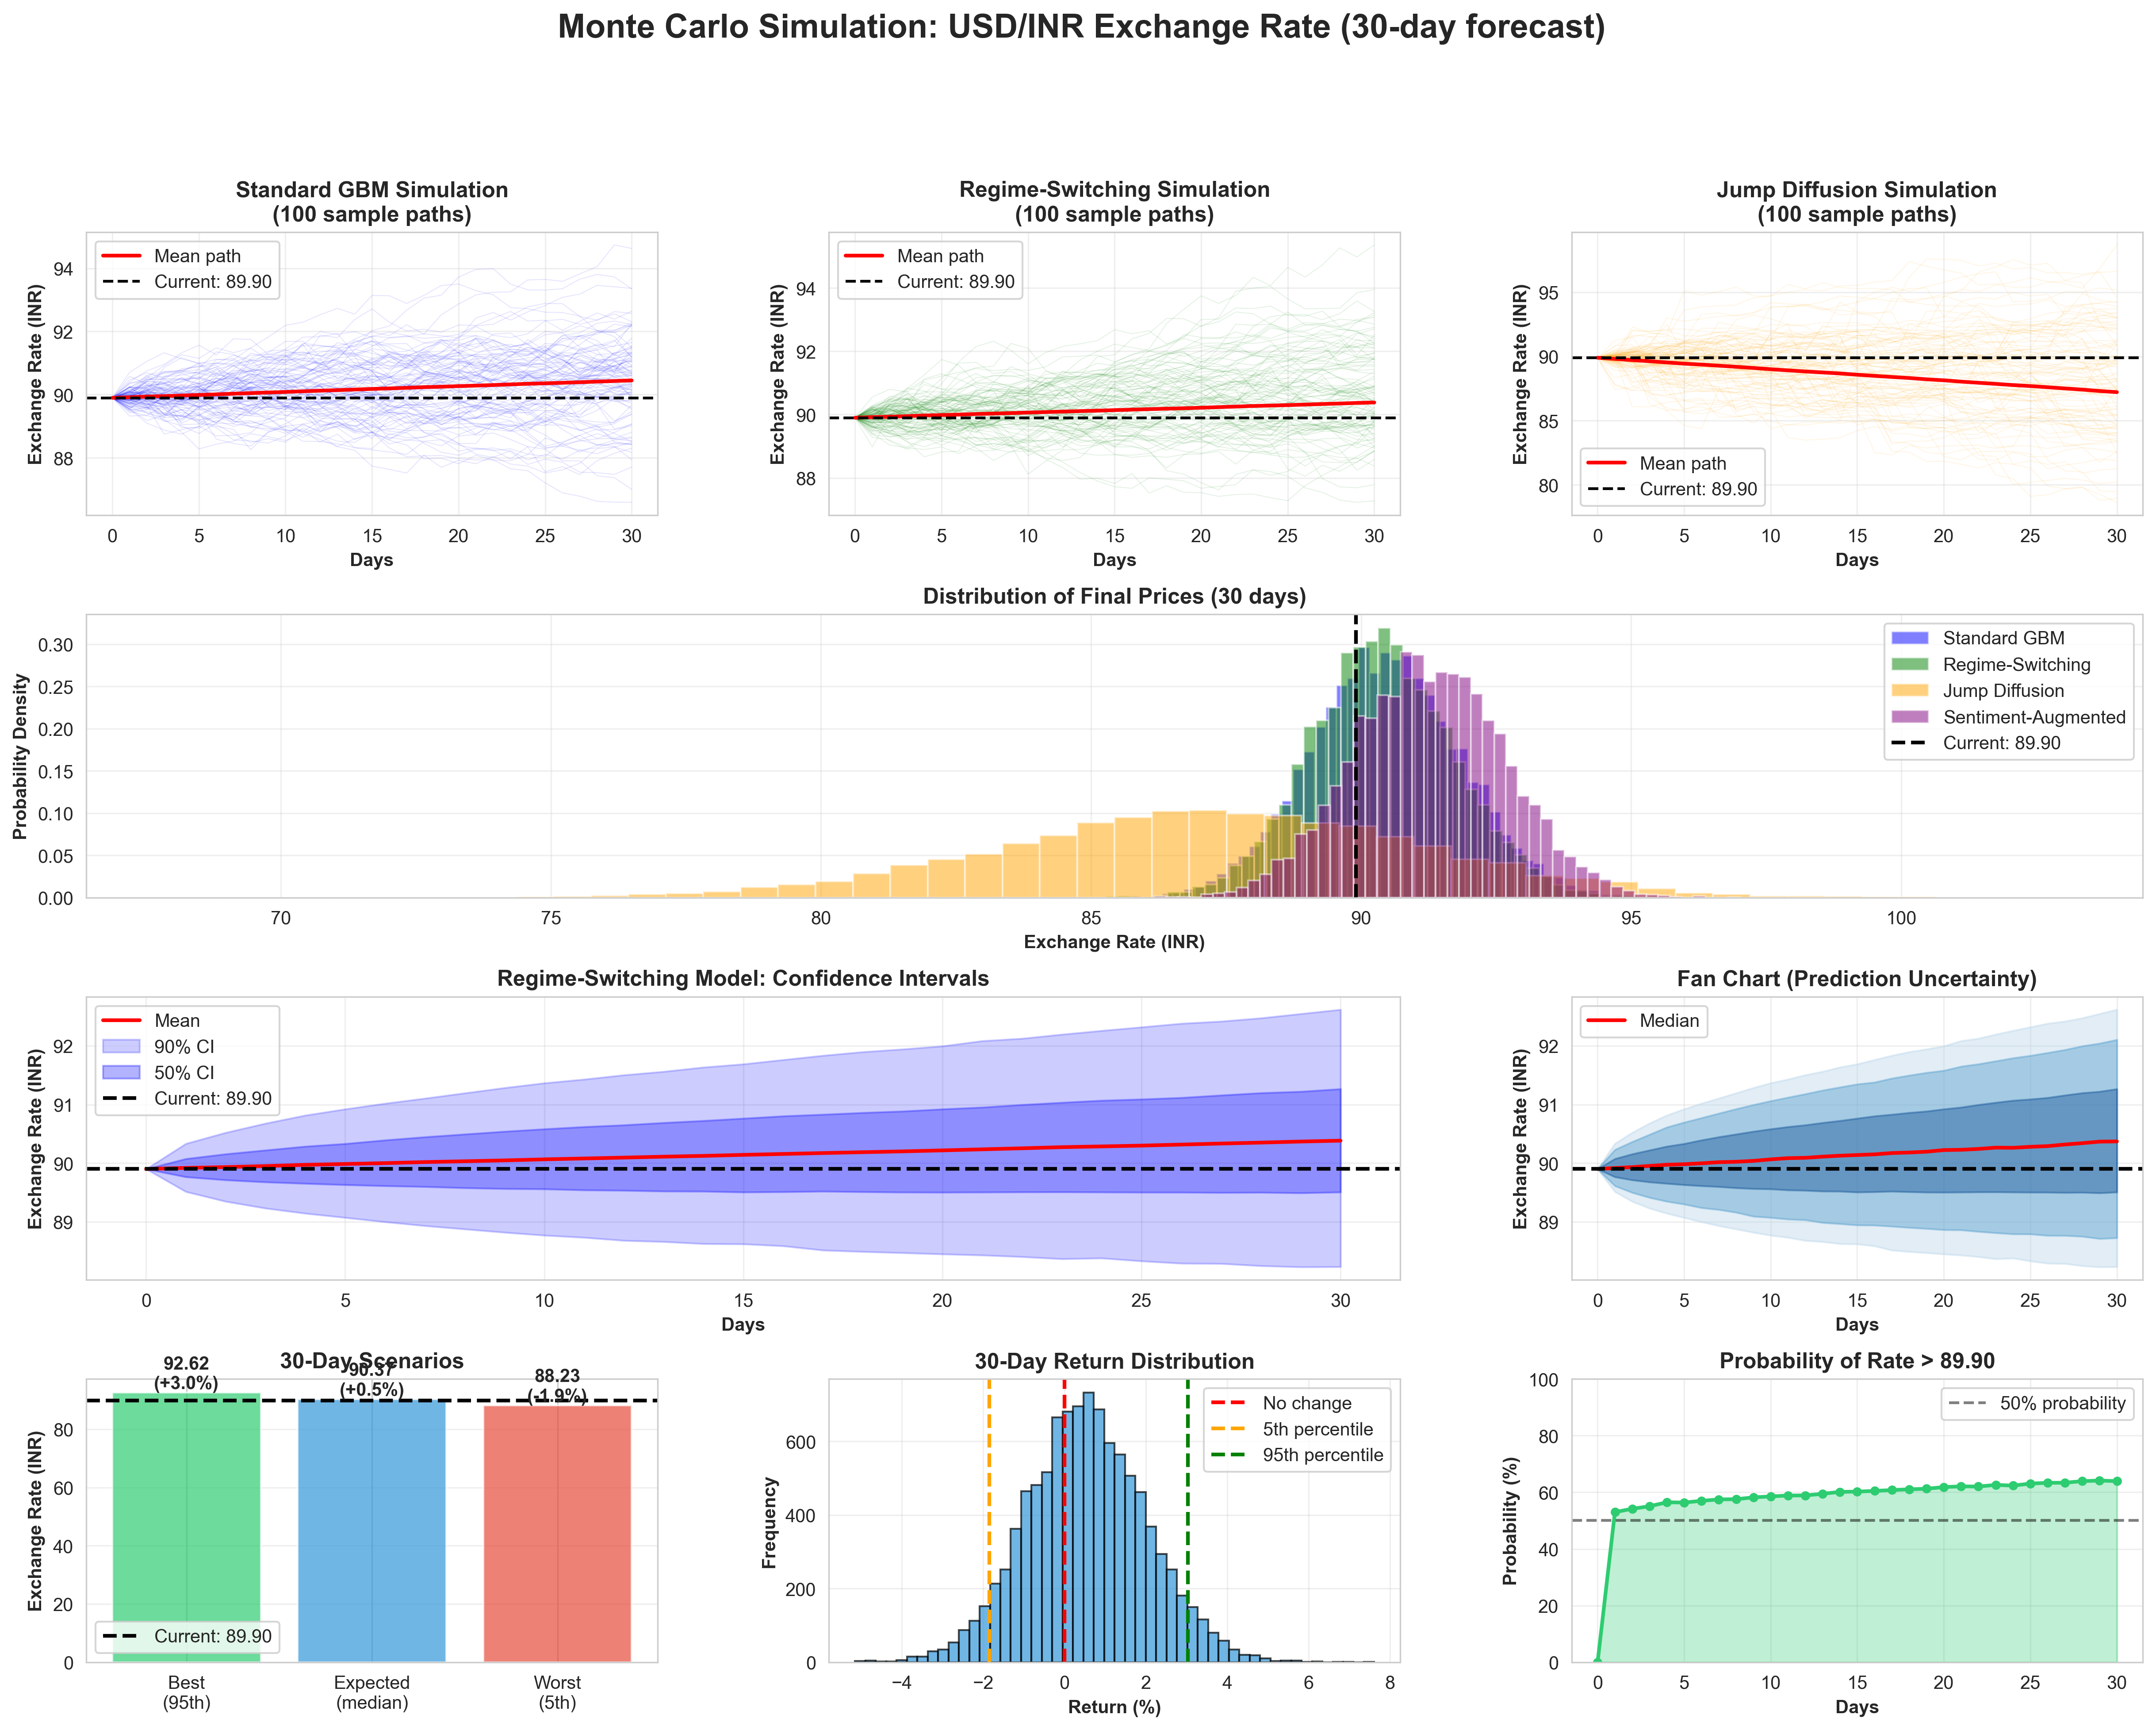
\includegraphics[width=\linewidth]{monte_carlo_results.png}
    \caption{Full Monte Carlo results panel.}
\end{subfigure}
\caption{Additional quantitative branch diagnostics.}
\end{figure*}

\begin{figure*}[p]
\centering
\begin{subfigure}[t]{0.48\textwidth}
    \centering
    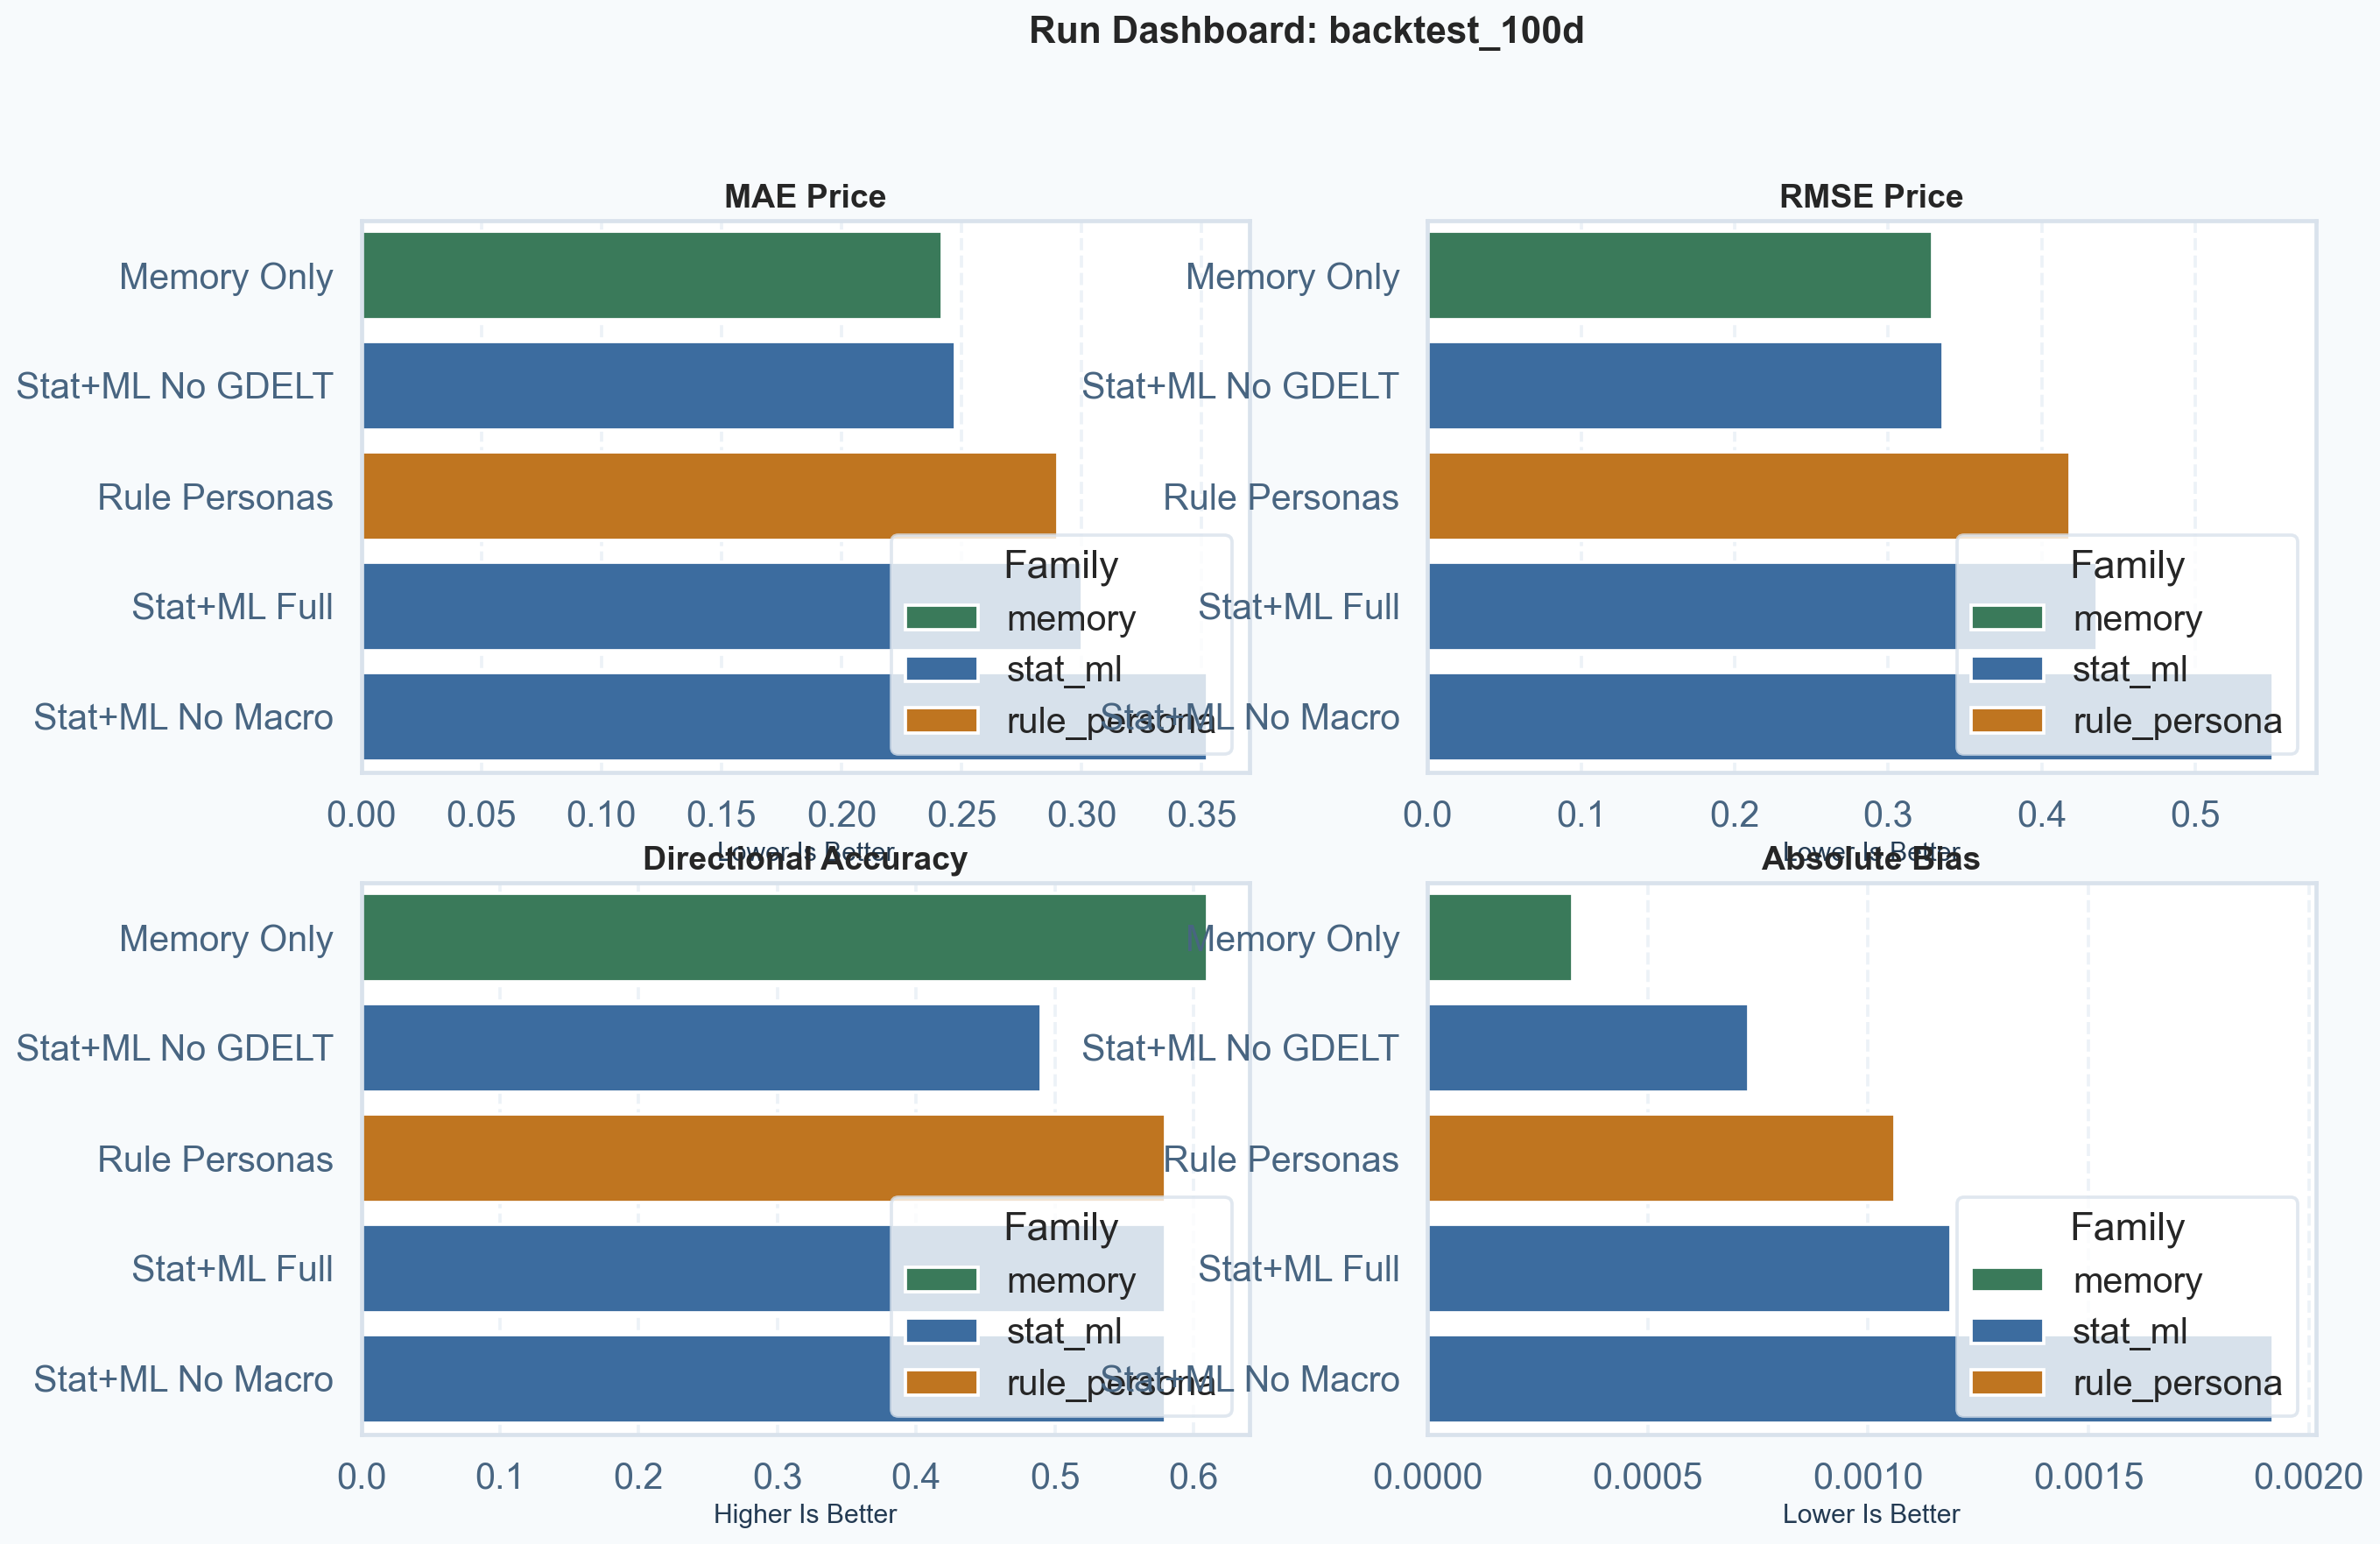
\includegraphics[width=\linewidth]{final_phase_dashboard_100d.png}
    \caption{\texttt{final phase} 100-day dashboard.}
\end{subfigure}
\hfill
\begin{subfigure}[t]{0.48\textwidth}
    \centering
    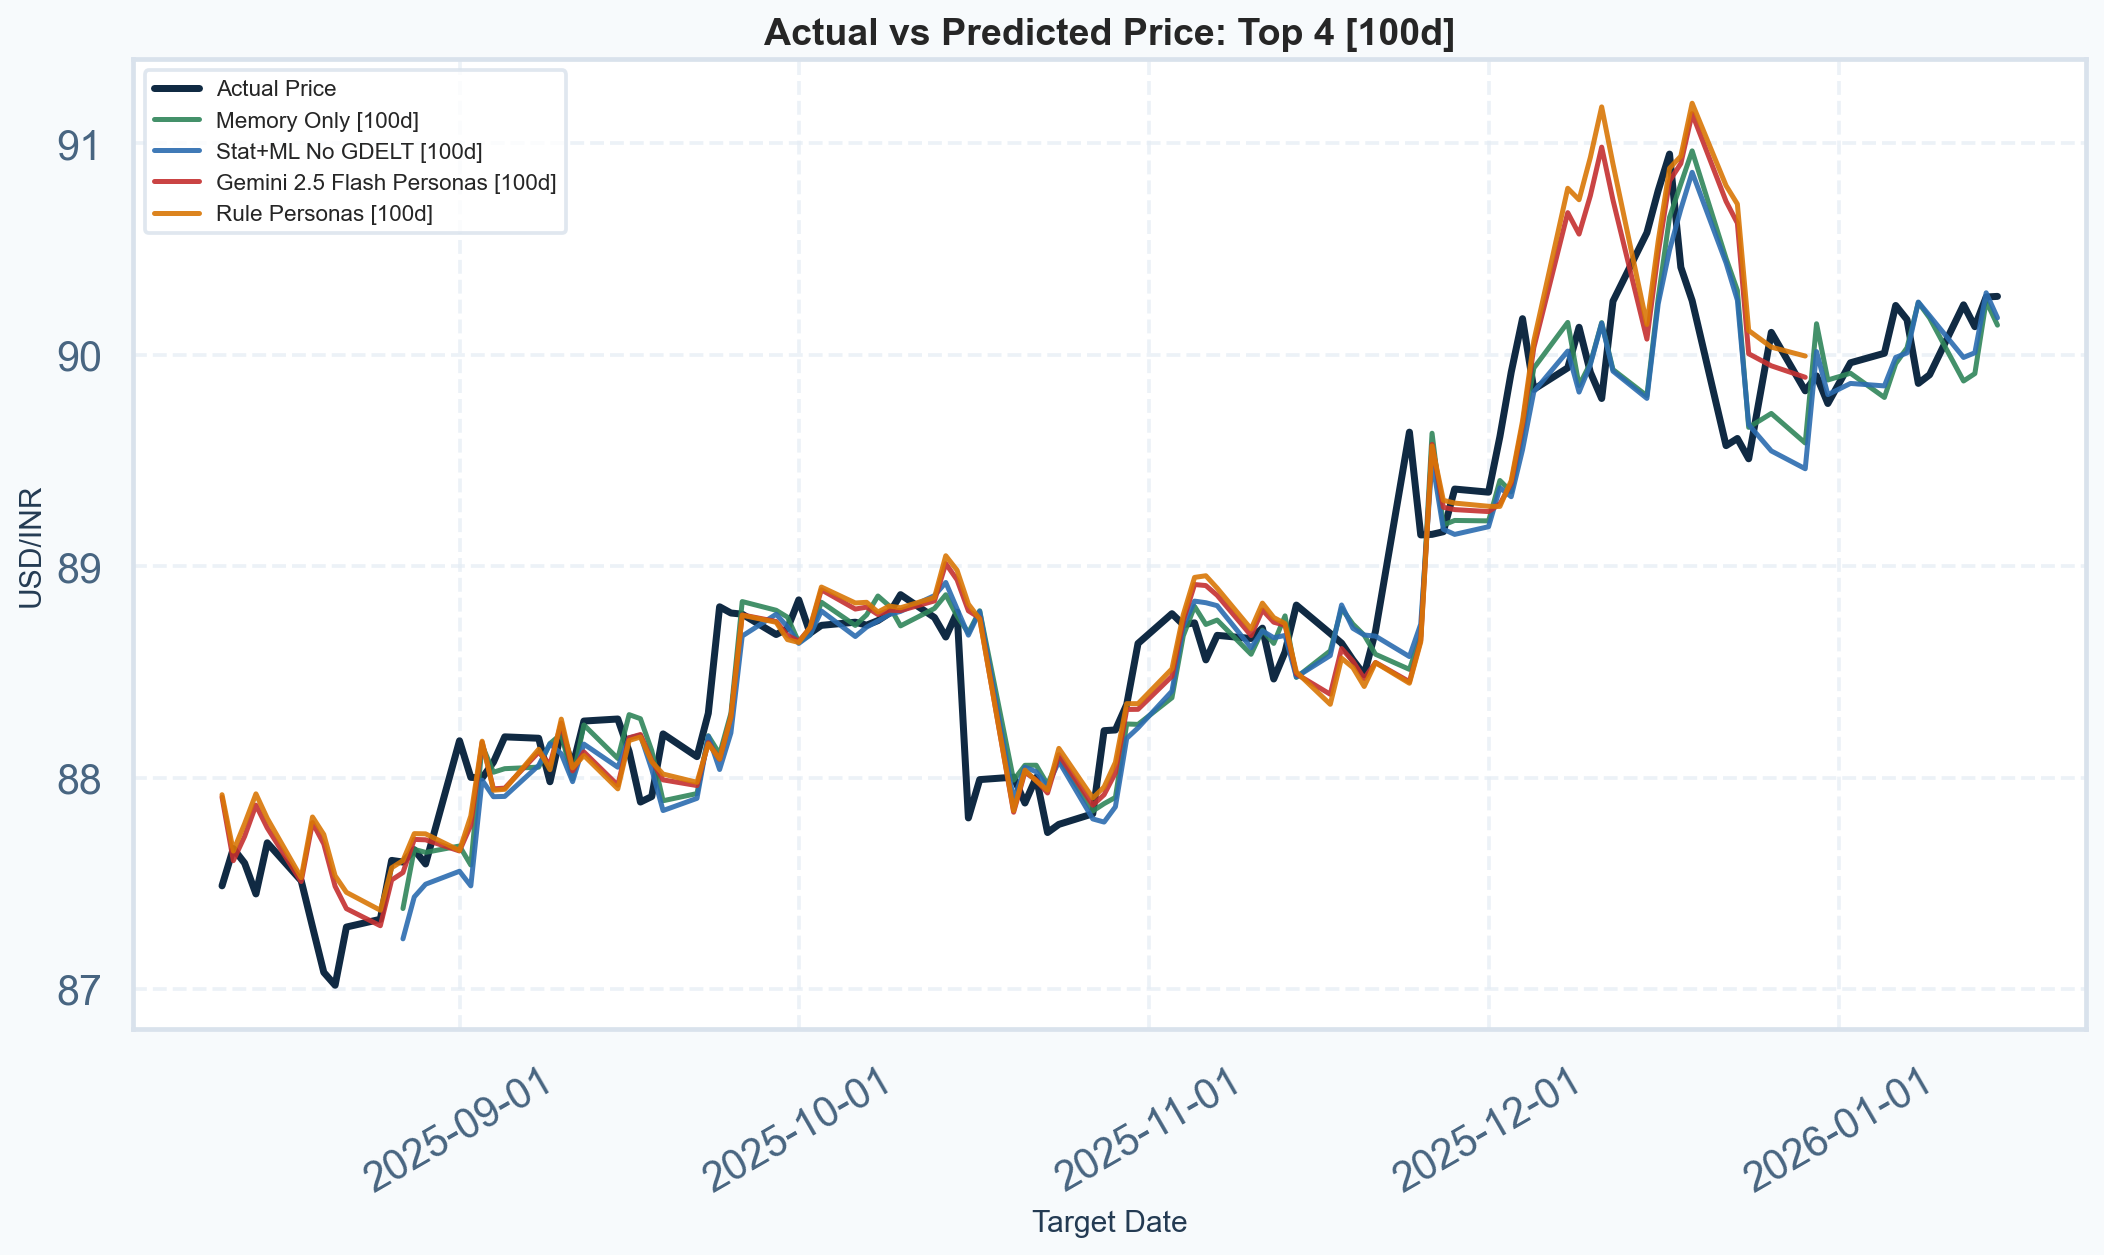
\includegraphics[width=\linewidth]{final_phase_predictions_100d.png}
    \caption{Top 100-day prediction overlays.}
\end{subfigure}
\caption{Additional \texttt{final phase} plots.}
\end{figure*}

\begin{figure*}[p]
\centering
\begin{subfigure}[t]{0.48\textwidth}
    \centering
    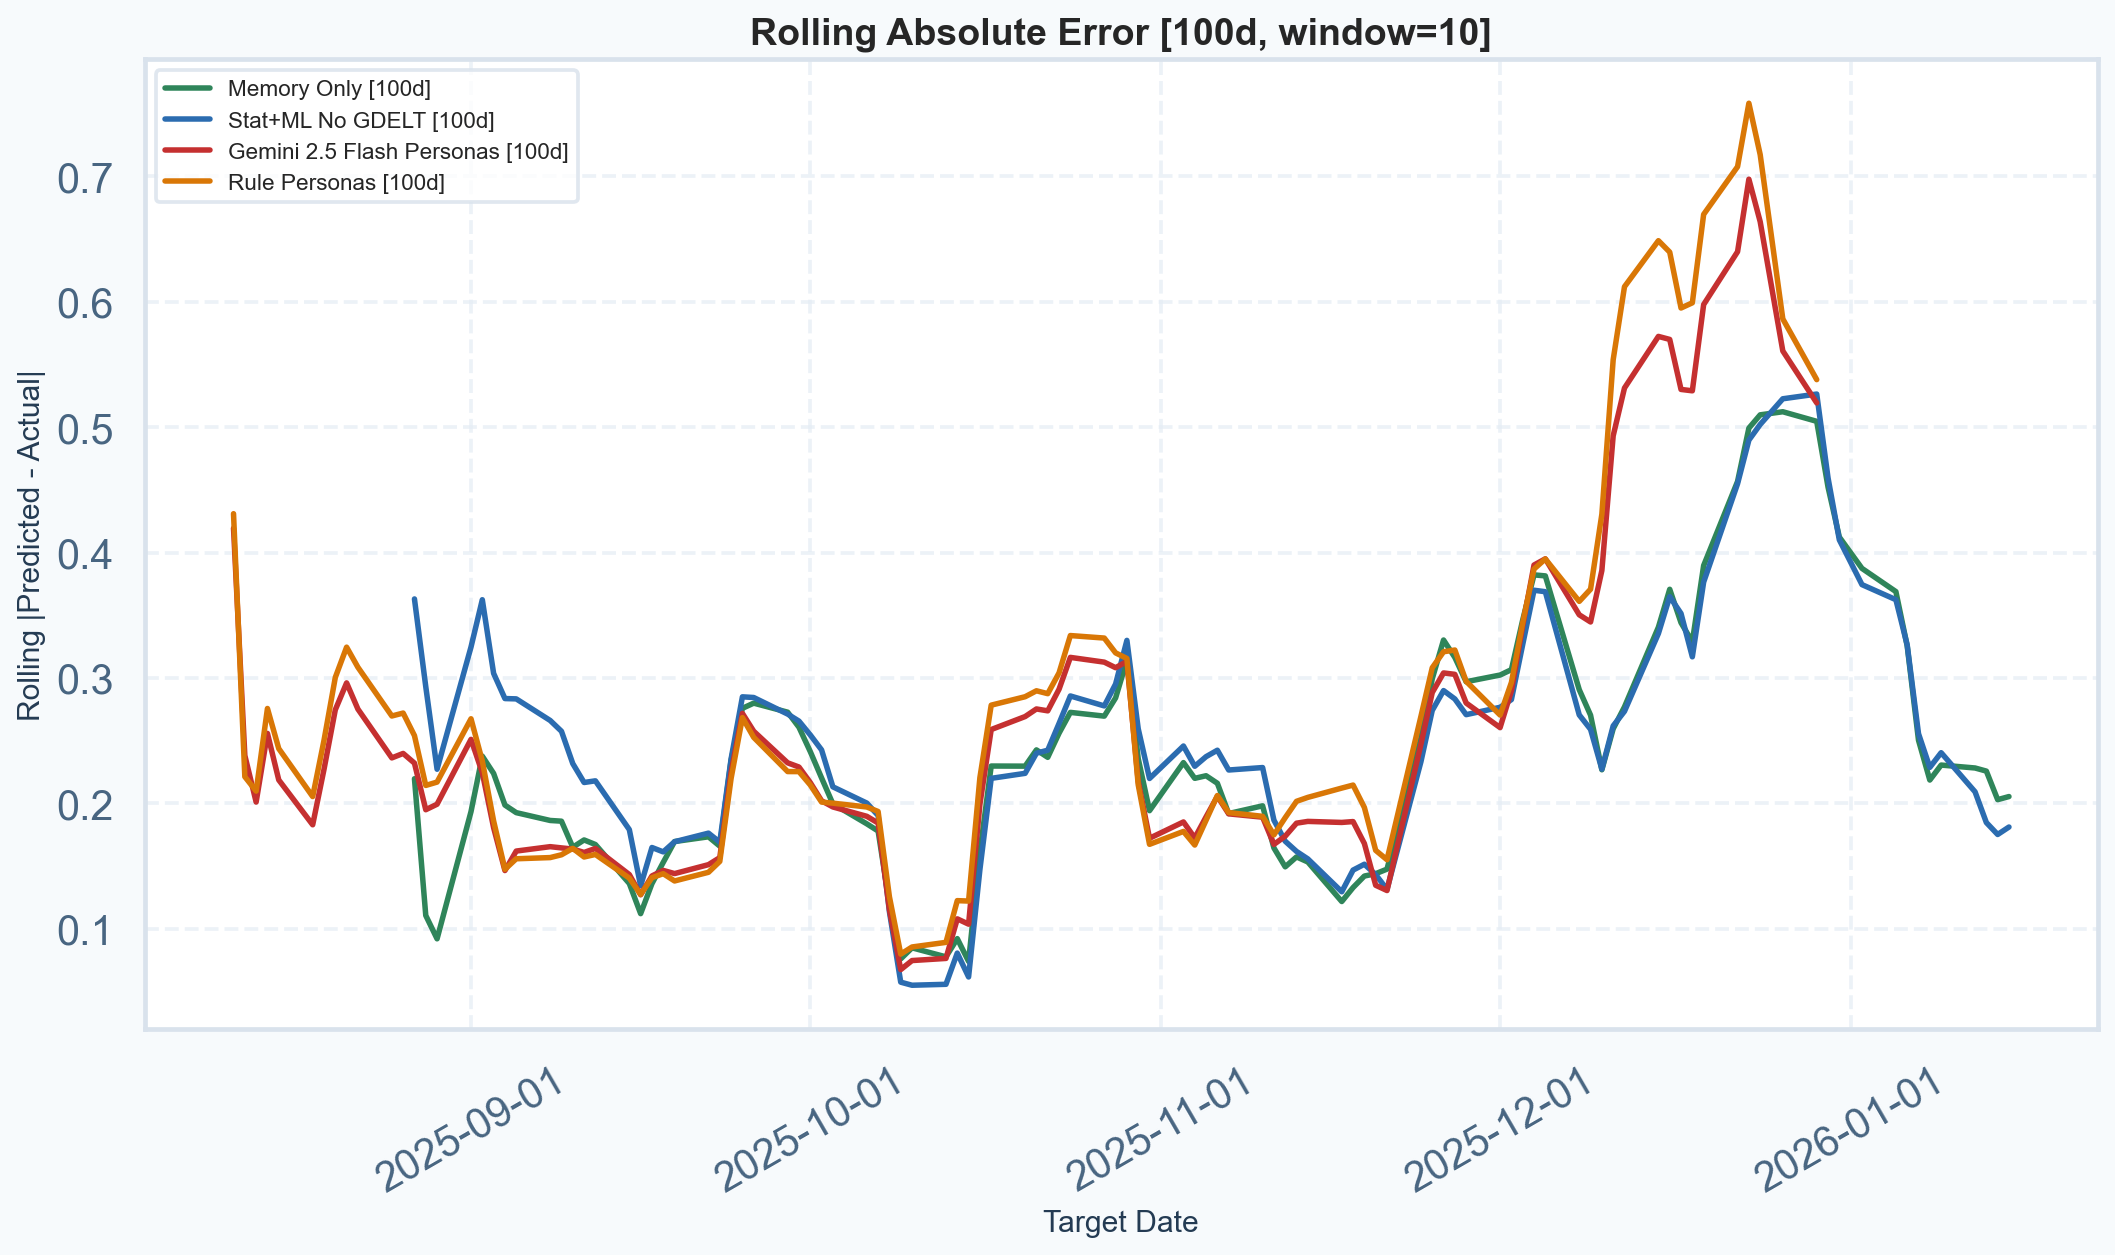
\includegraphics[width=\linewidth]{final_phase_rolling_100d.png}
    \caption{Rolling absolute error over 100 days.}
\end{subfigure}
\hfill
\begin{subfigure}[t]{0.48\textwidth}
    \centering
    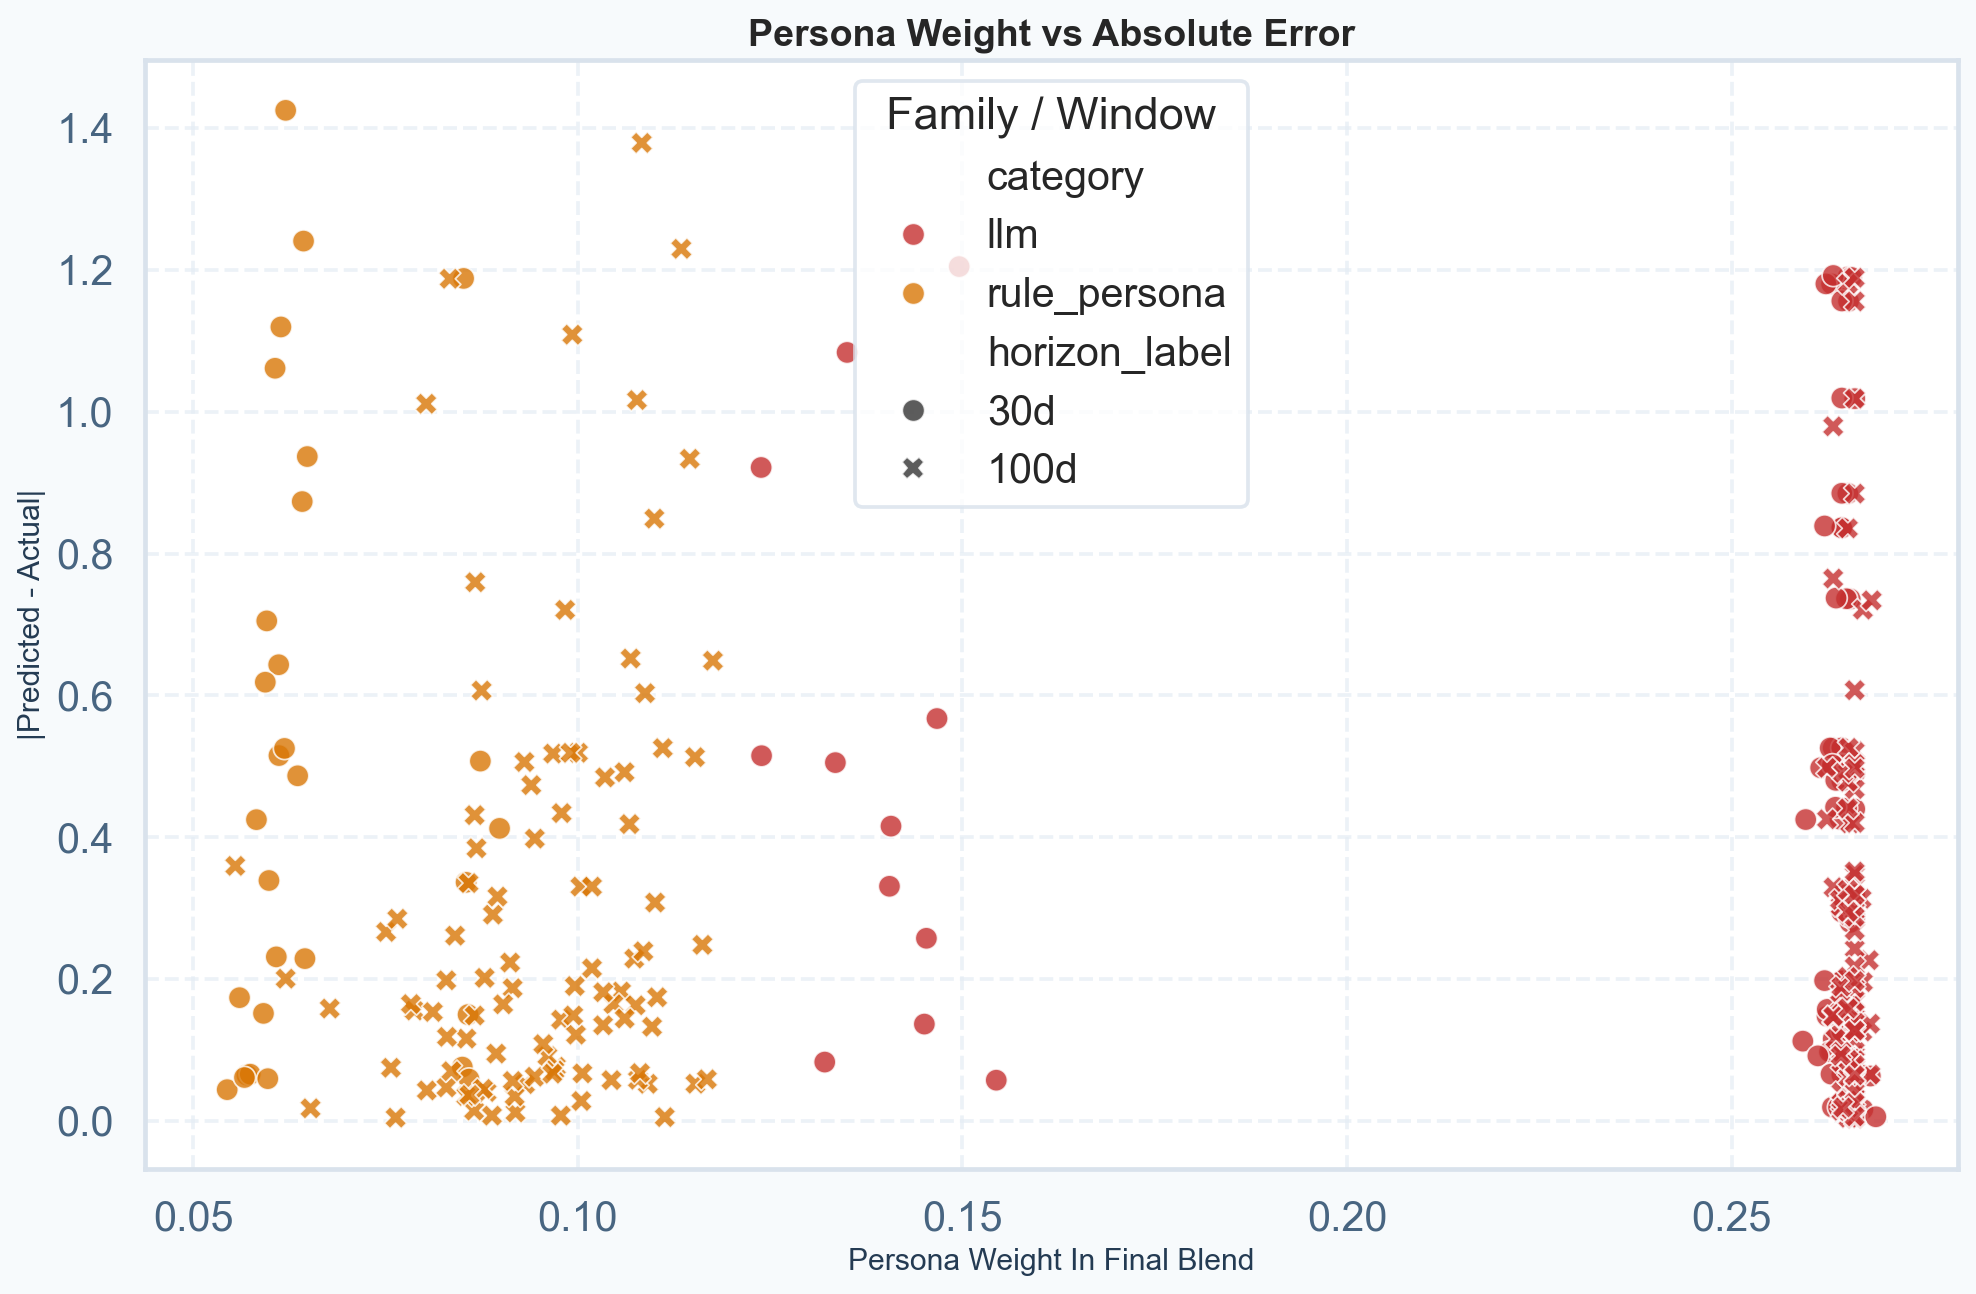
\includegraphics[width=\linewidth]{final_phase_persona_weight.png}
    \caption{Persona weight versus error relationship.}
\end{subfigure}
\caption{Late-stage diagnostics from the market-memory branch.}
\end{figure*}

\begin{figure*}[p]
\centering
\begin{subfigure}[t]{0.48\textwidth}
    \centering
    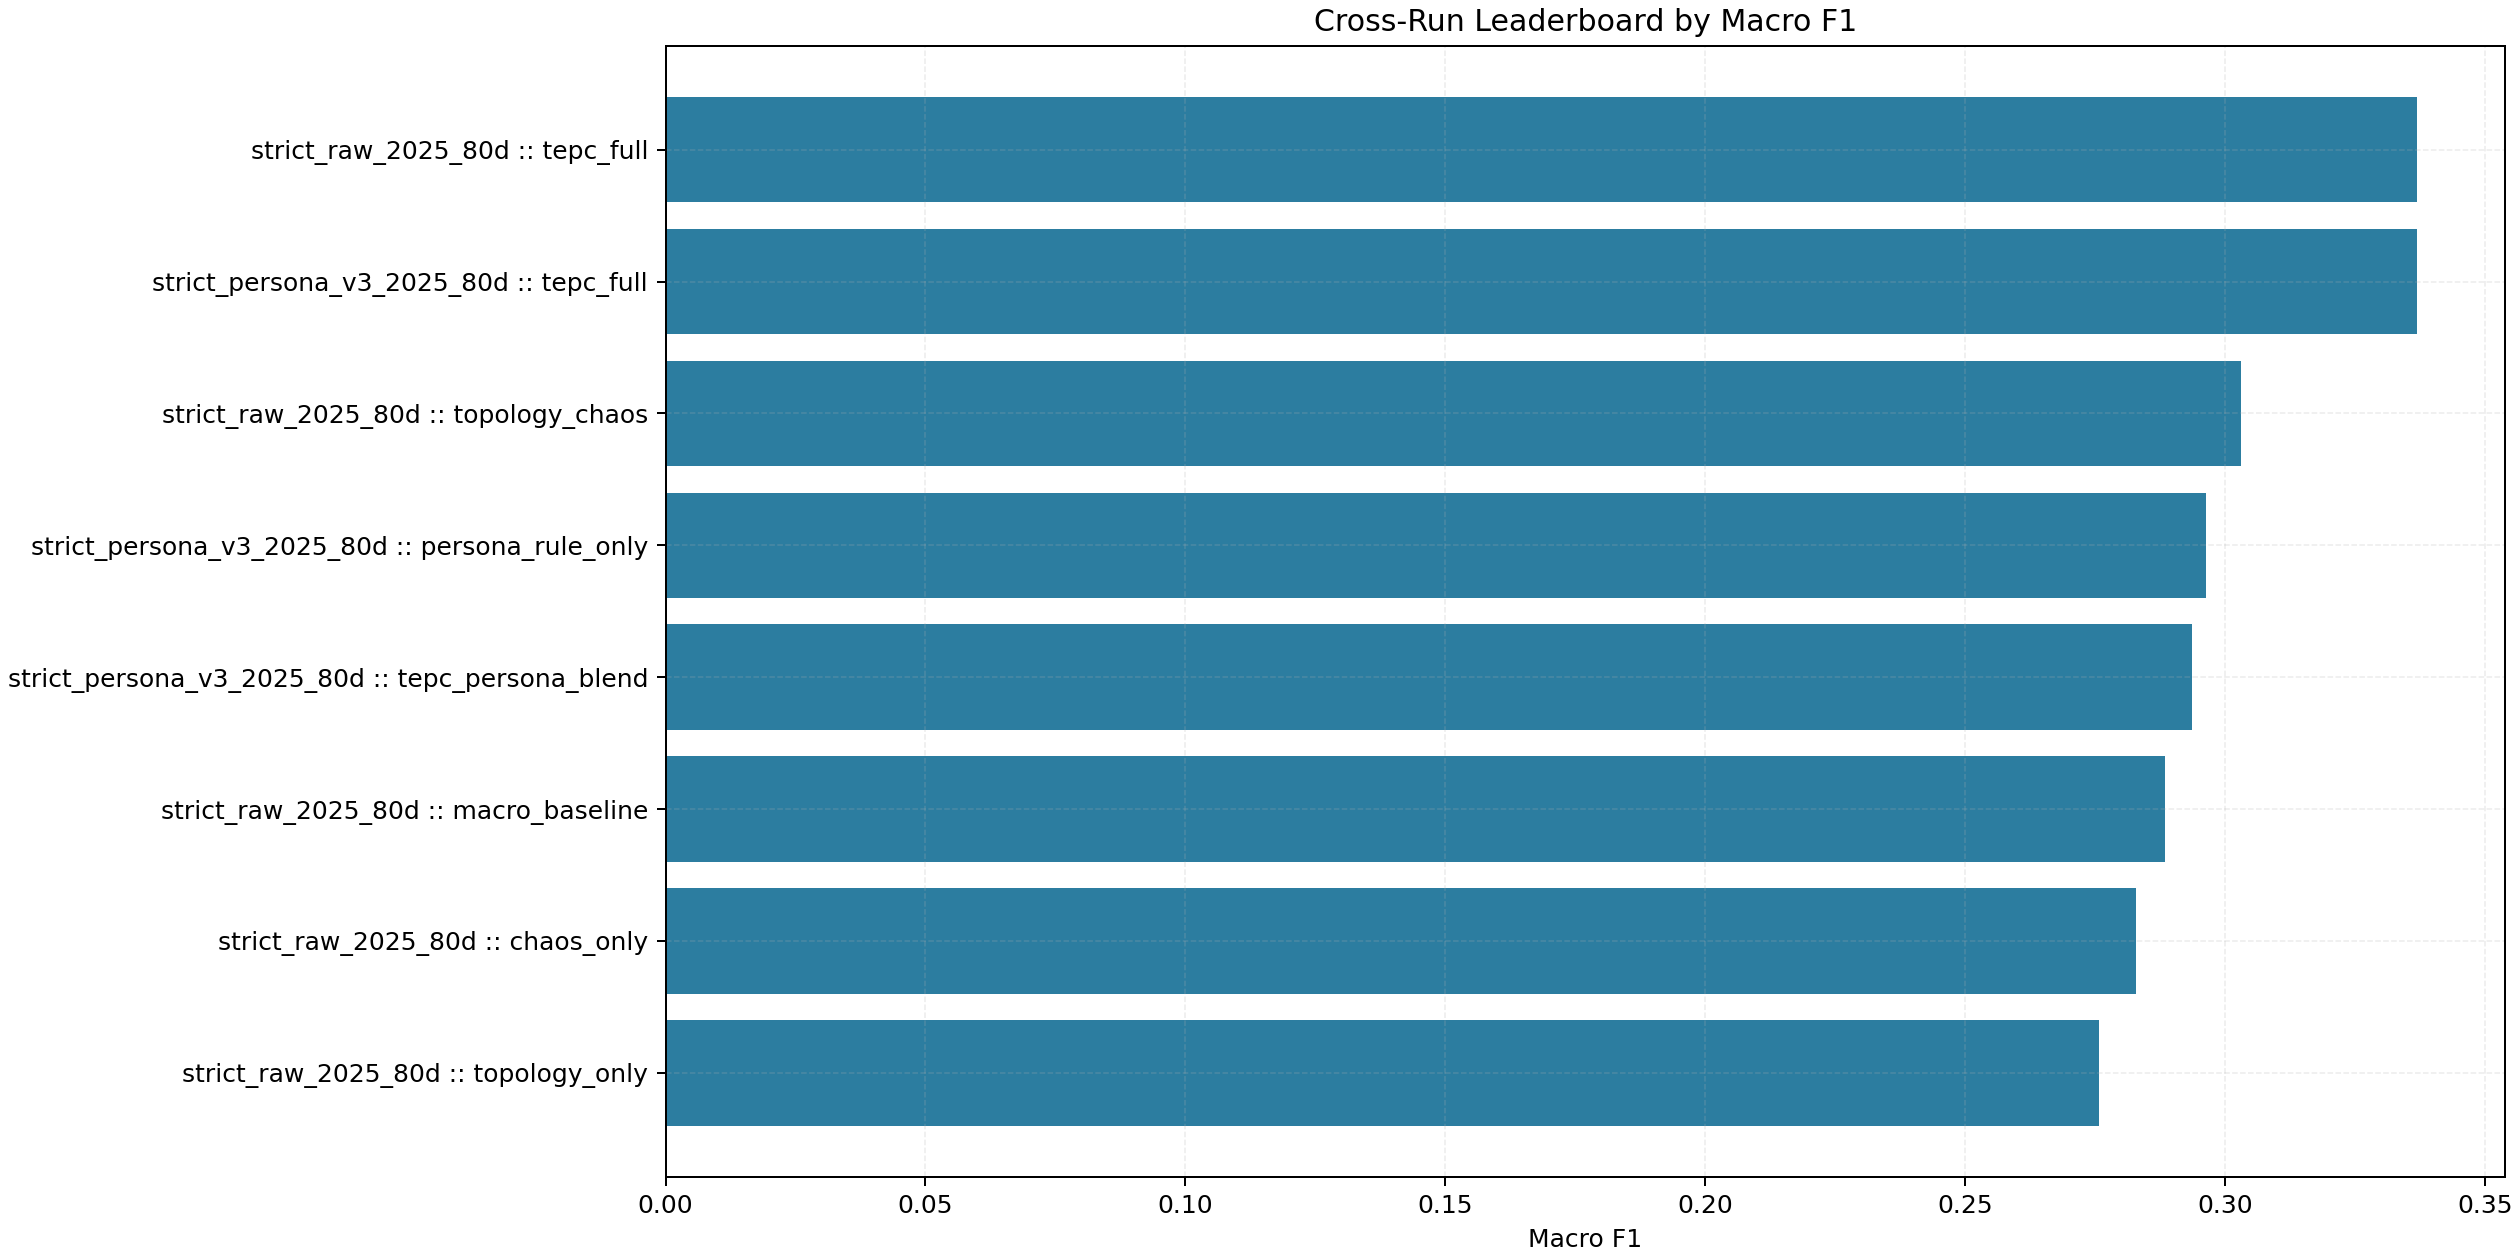
\includegraphics[width=\linewidth]{tepc_compare_leaderboard.png}
    \caption{TEPC cross-run leaderboard.}
\end{subfigure}
\hfill
\begin{subfigure}[t]{0.48\textwidth}
    \centering
    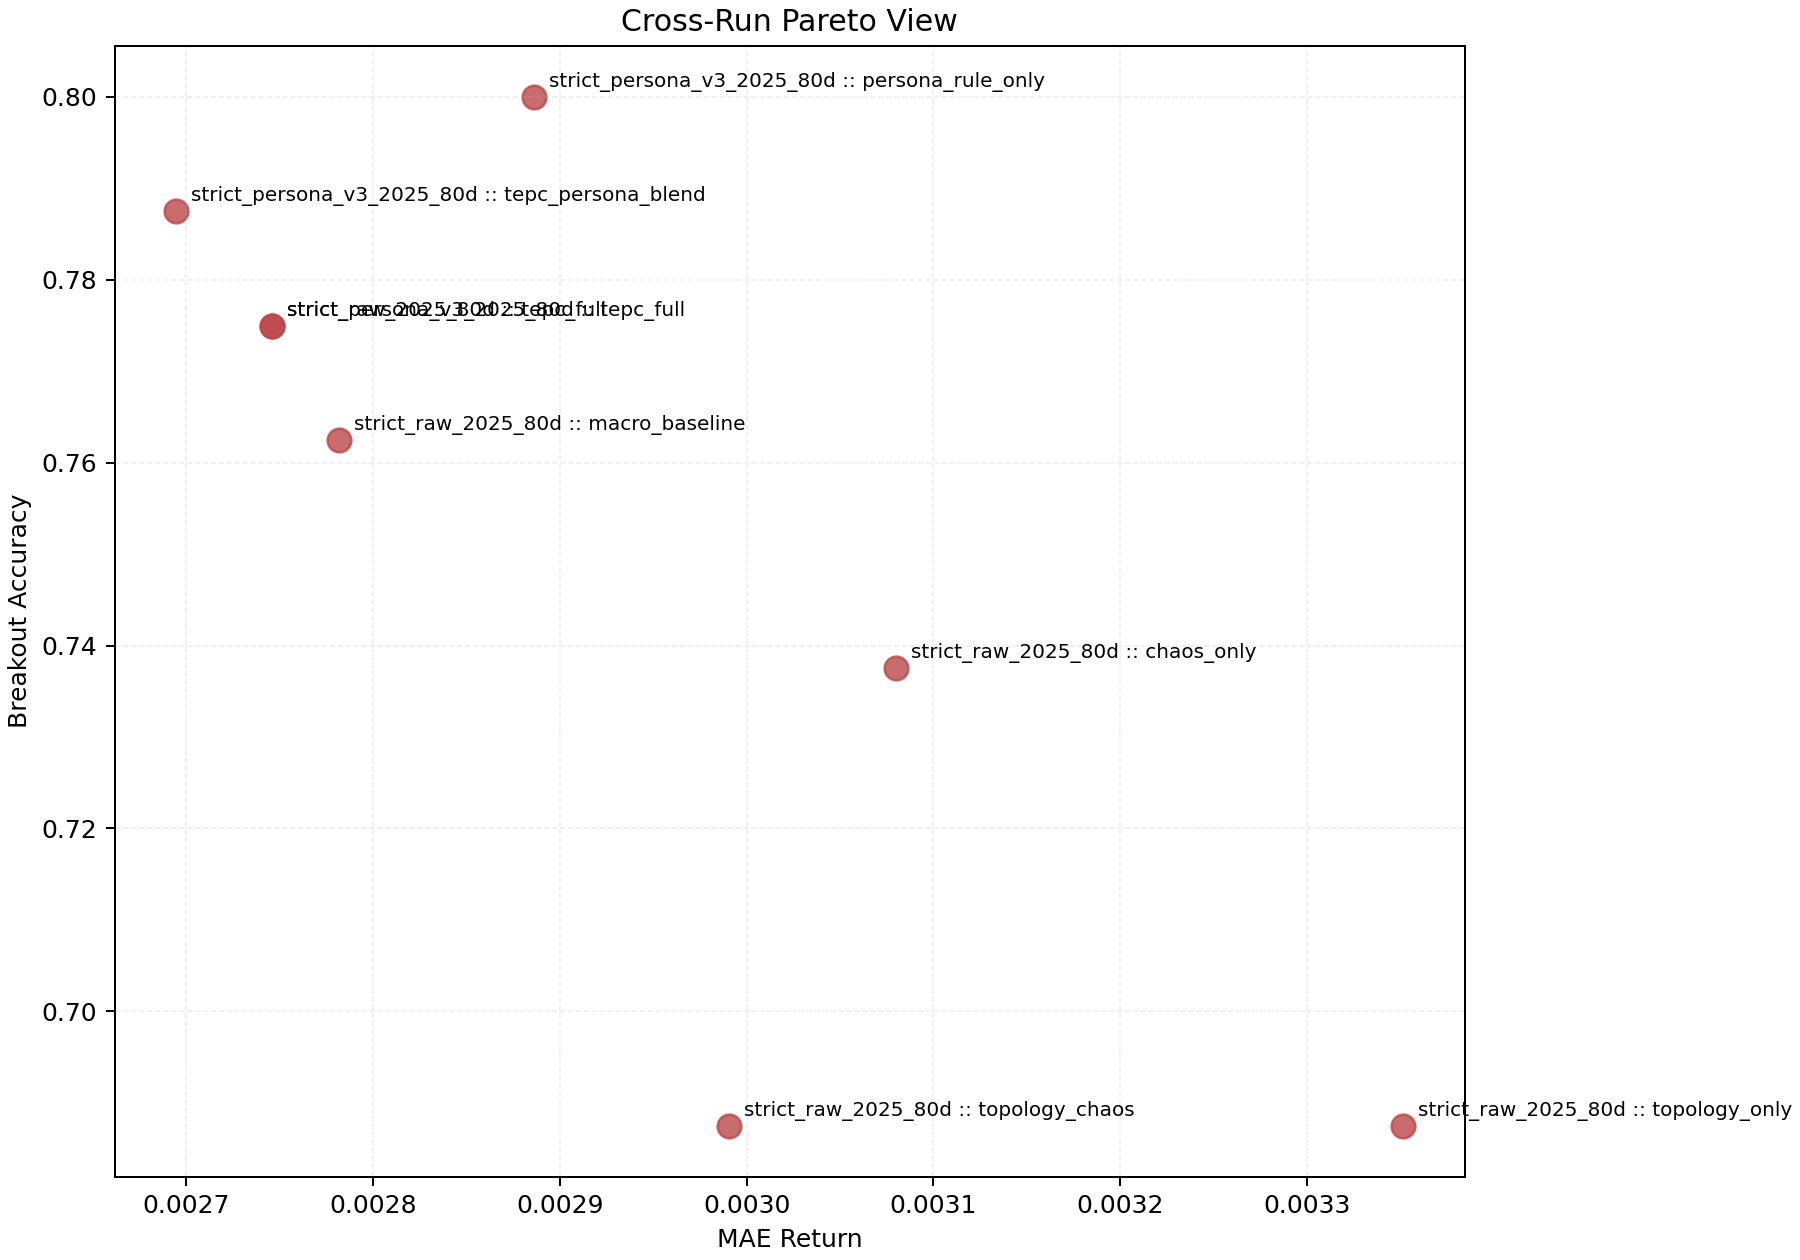
\includegraphics[width=\linewidth]{tepc_compare_pareto.png}
    \caption{TEPC cross-run Pareto comparison.}
\end{subfigure}
\caption{Additional TEPC comparison plots across strict raw and persona-overlay runs.}
\end{figure*}

\begin{figure*}[p]
\centering
\begin{subfigure}[t]{0.48\textwidth}
    \centering
    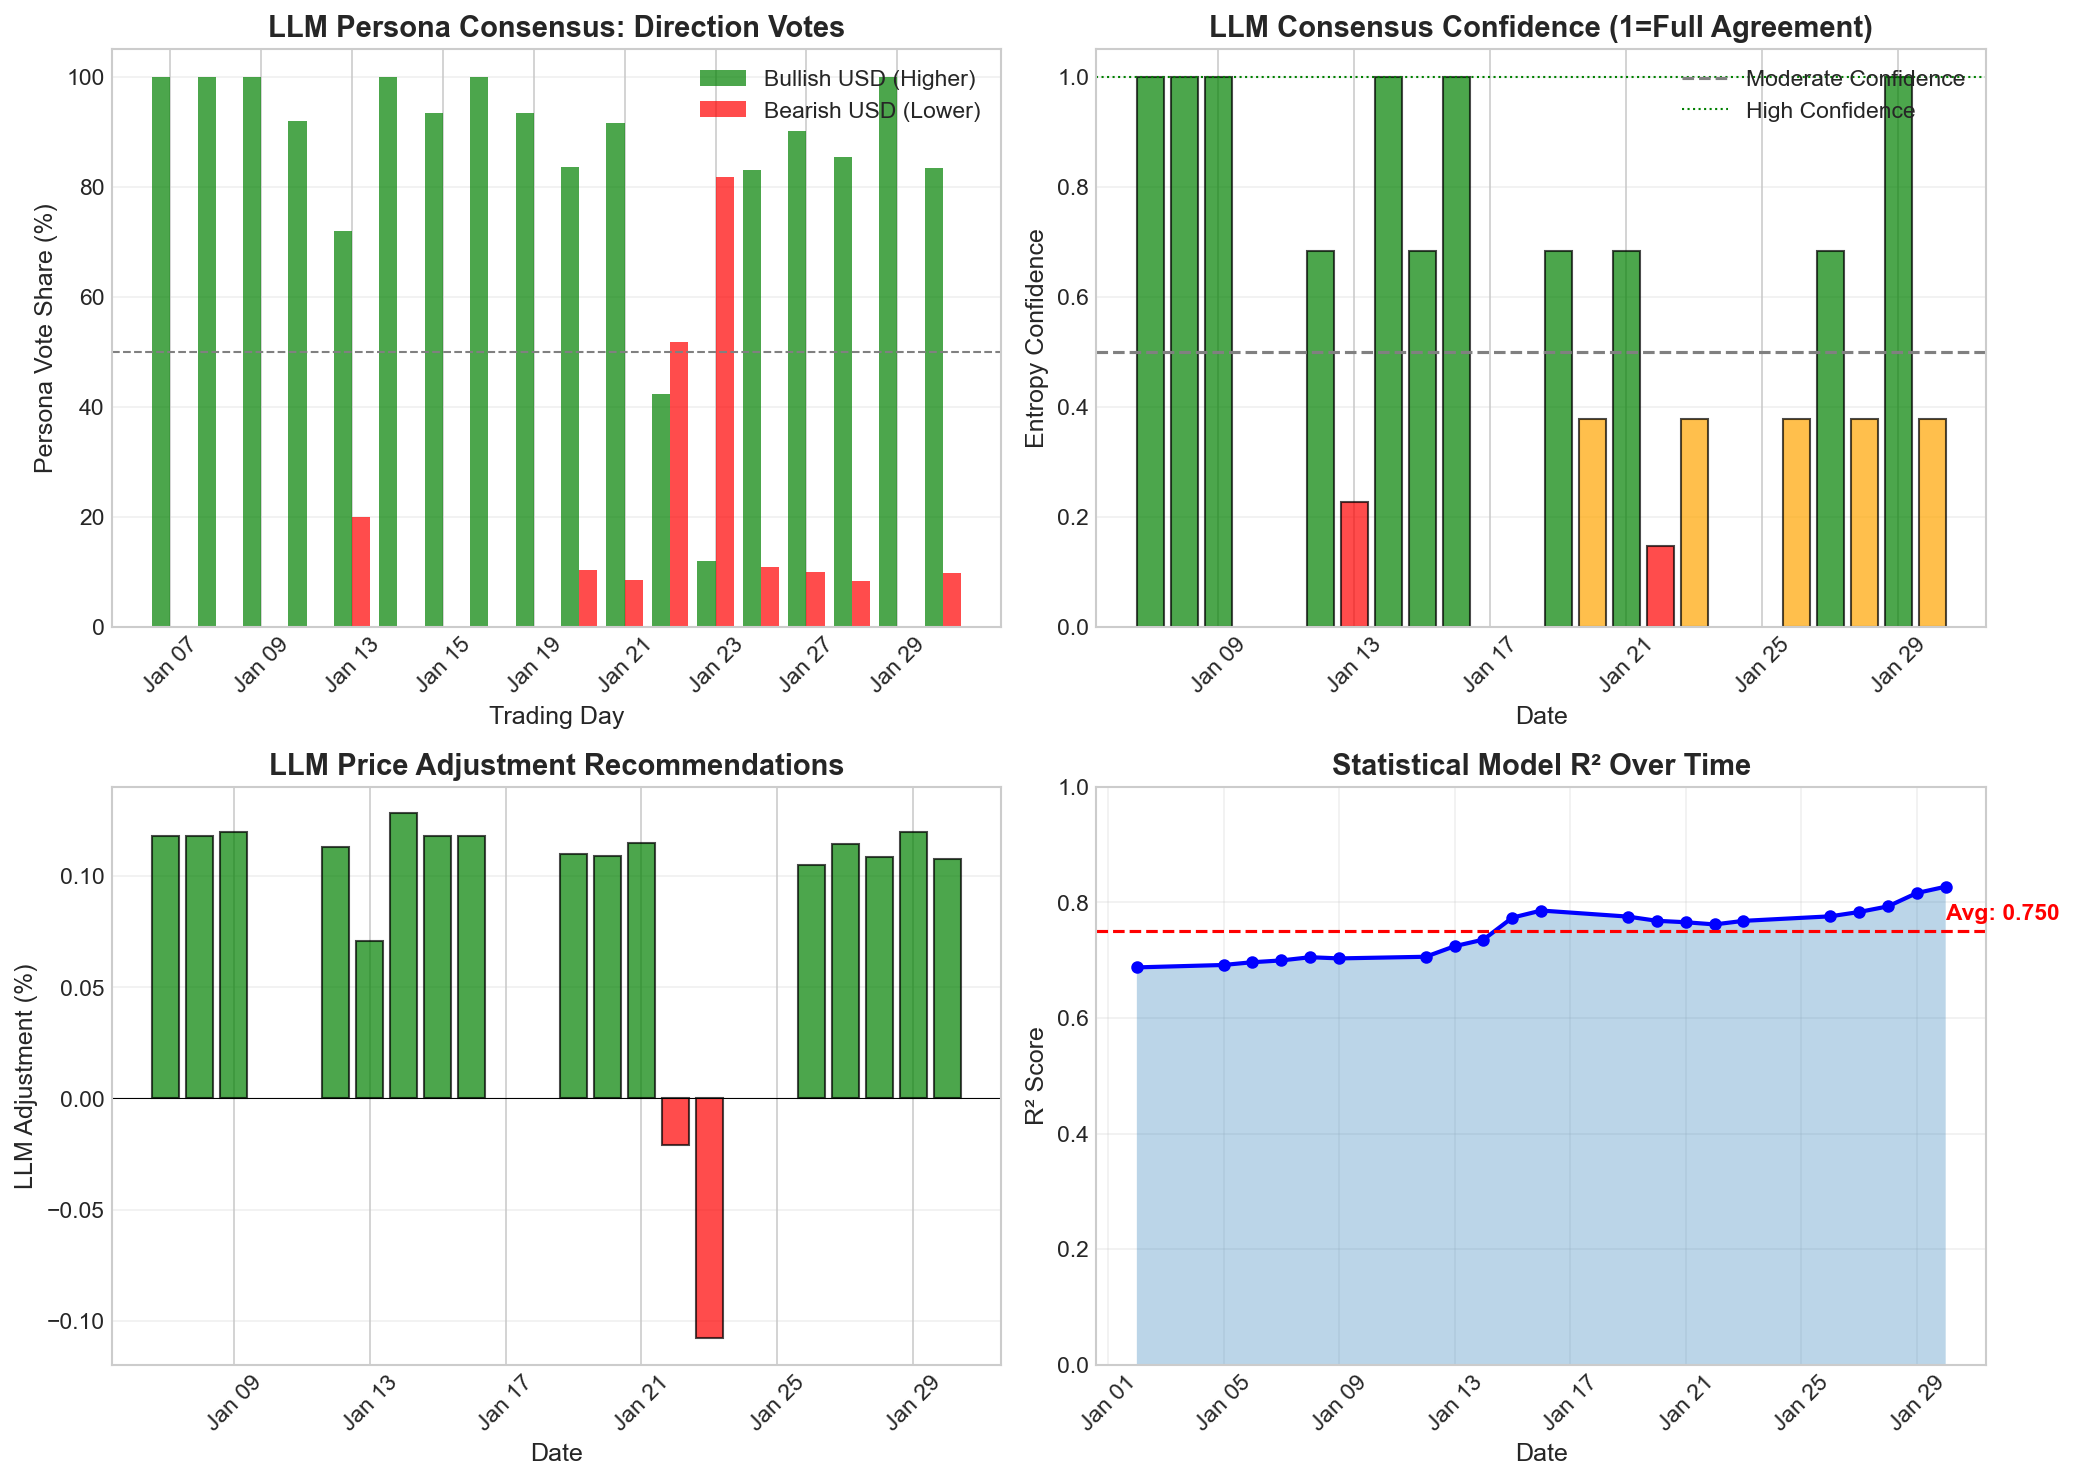
\includegraphics[width=\linewidth]{gemini_v4_jan_llm.png}
    \caption{Gemini January 2026 LLM analysis panel.}
\end{subfigure}
\hfill
\begin{subfigure}[t]{0.48\textwidth}
    \centering
    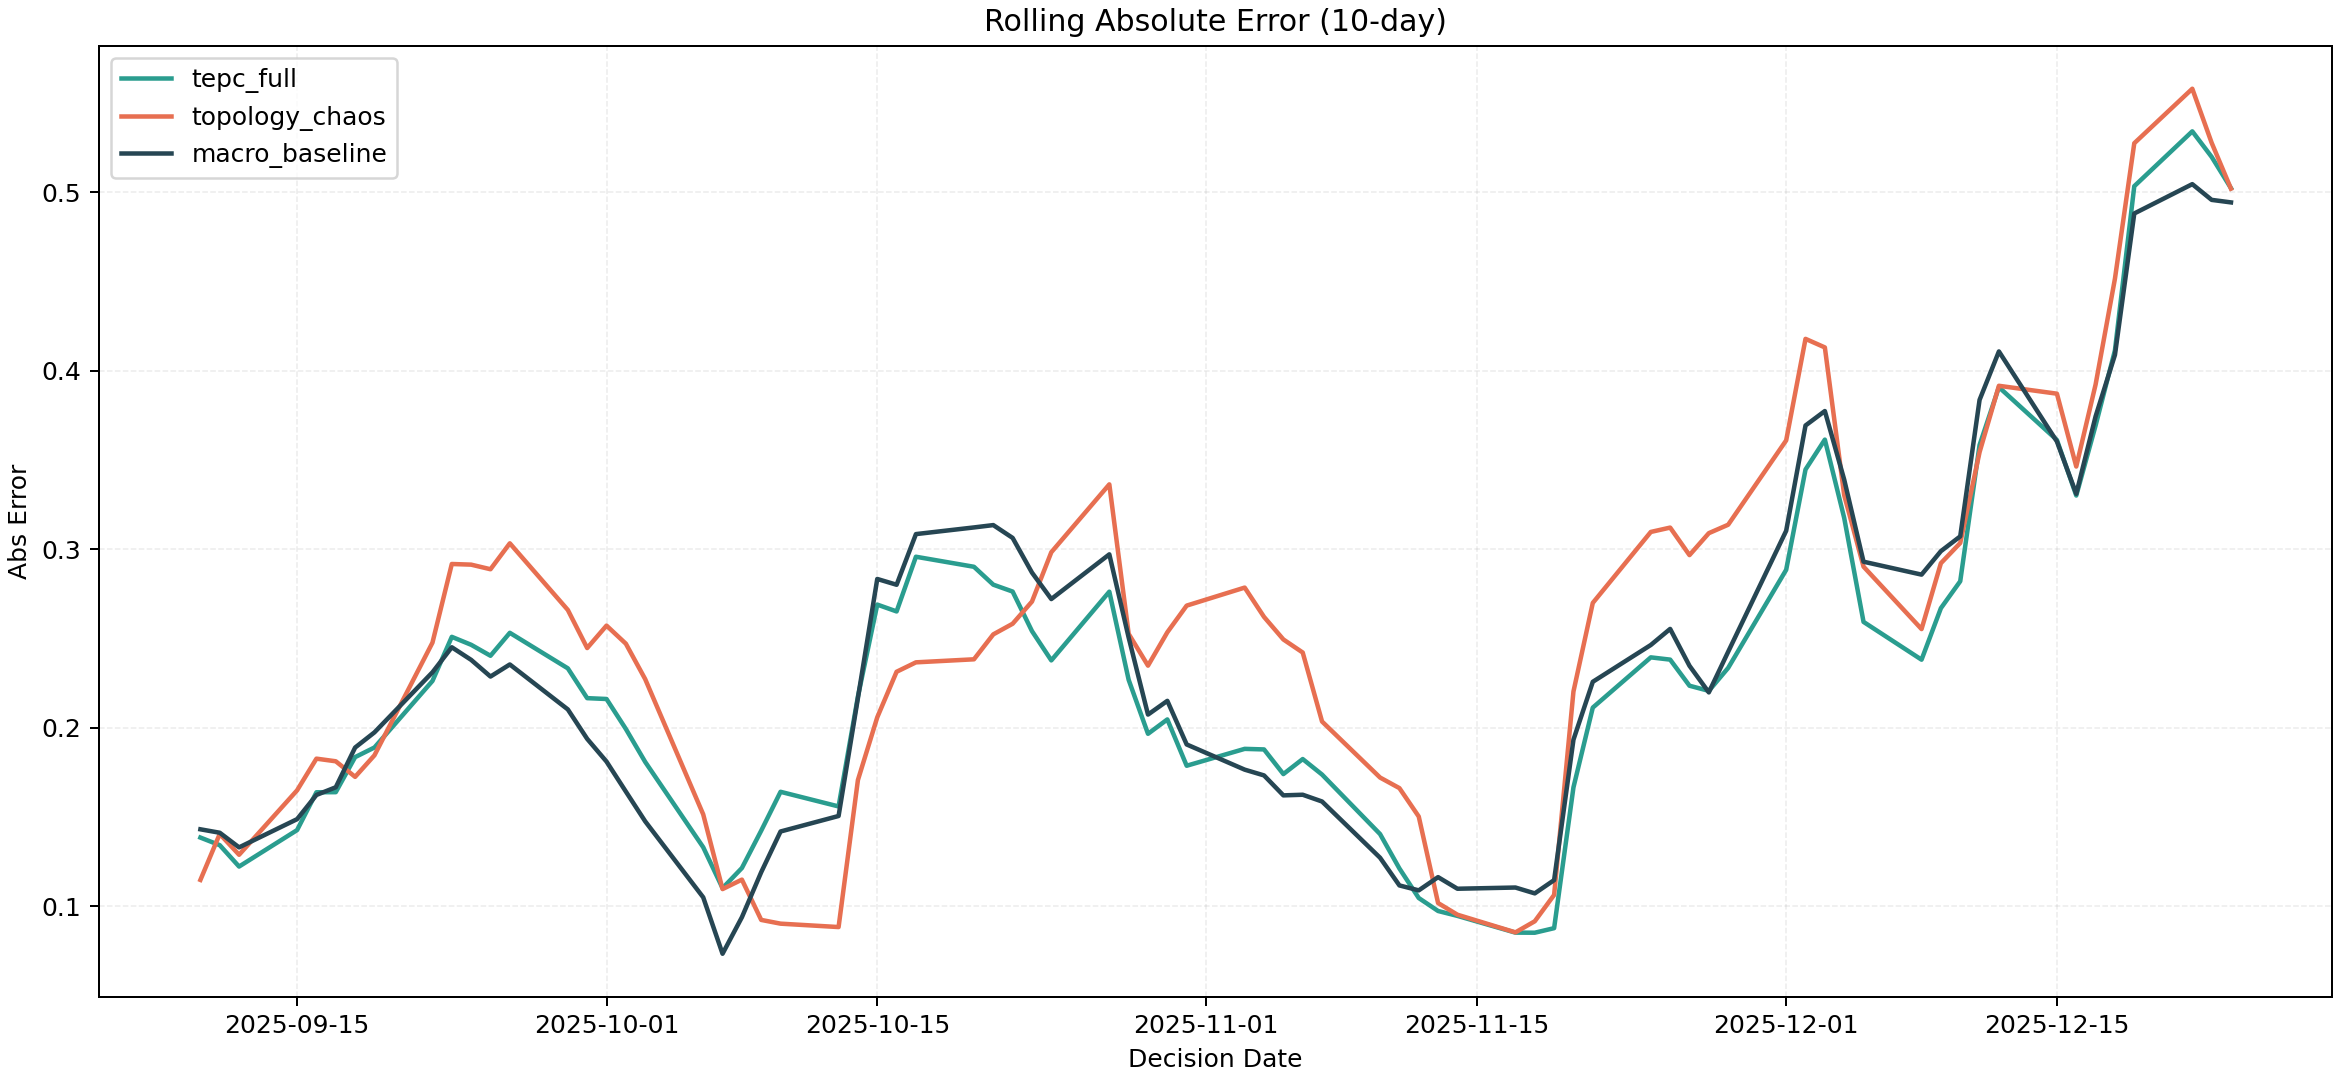
\includegraphics[width=\linewidth]{tepc_strict_rolling_error.png}
    \caption{TEPC strict rolling absolute error comparison.}
\end{subfigure}
\caption{Additional diagnostics for the LLM and topology-chaos branches.}
\end{figure*}

% ============================================================
% REFERENCES
% ============================================================
\bibliographystyle{apalike}

\begin{thebibliography}{99}

\bibitem[Baker \& Wurgler, 2007]{baker2007}
Baker, M., \& Wurgler, J. (2007).
Investor sentiment in the stock market.
\textit{Journal of Economic Perspectives}, 21(2), 129--151.

\bibitem[BIS, 2022]{bis2022}
Bank for International Settlements. (2022).
Triennial Central Bank Survey of Foreign Exchange and OTC Derivatives Markets.
\textit{BIS Statistical Release}.

\bibitem[Bollerslev, 1986]{bollerslev1986}
Bollerslev, T. (1986).
Generalized autoregressive conditional heteroskedasticity.
\textit{Journal of Econometrics}, 31(3), 307--327.

\bibitem[Bollen et al., 2011]{bollen2011}
Bollen, J., Mao, H., \& Zeng, X. (2011).
Twitter mood predicts the stock market.
\textit{Journal of Computational Science}, 2(1), 1--8.

\bibitem[Chen \& Guestrin, 2016]{chen2016xgboost}
Chen, T., \& Guestrin, C. (2016).
XGBoost: A scalable tree boosting system.
In \textit{Proceedings of the 22nd ACM SIGKDD International Conference on Knowledge Discovery and Data Mining}, 785--794.

\bibitem[Clemen, 1989]{clemen1989}
Clemen, R. T. (1989).
Combining forecasts: A review and annotated bibliography.
\textit{International Journal of Forecasting}, 5(4), 559--583.

\bibitem[Condorcet, 1785]{condorcet1785}
de Condorcet, M. (1785).
\textit{Essai sur l'application de l'analyse \`a la probabilit\'e des d\'ecisions rendues \`a la pluralit\'e des voix}.
Paris: Imprimerie Royale.

\bibitem[Dragomiretskiy \& Zosso, 2014]{dragomiretskiy2014}
Dragomiretskiy, K., \& Zosso, D. (2014).
Variational mode decomposition.
\textit{IEEE Transactions on Signal Processing}, 62(3), 531--544.

\bibitem[Engel \& West, 2005]{engel2014}
Engel, C., \& West, K. D. (2005).
Exchange rates and fundamentals.
\textit{Journal of Political Economy}, 113(3), 485--517.

\bibitem[Galeshchuk, 2016]{galeshchuk2016}
Galeshchuk, S. (2016).
Neural networks performance in exchange rate prediction.
\textit{Neurocomputing}, 172, 446--452.

\bibitem[Leetaru \& Schrodt, 2013]{leetaru2013}
Leetaru, K., \& Schrodt, P. A. (2013).
GDELT: Global Data on Events, Language, and Tone, 1979--2012.
In \textit{International Studies Association Annual Convention}.

\bibitem[Li et al., 2024]{li2024llm}
Li, Y., et al. (2024).
Large language models for financial decision-making: A multi-agent perspective.
\textit{arXiv preprint arXiv:2402.xxxxx}.

\bibitem[Lopez-Lira \& Tang, 2023]{lopez2023}
Lopez-Lira, A., \& Tang, Y. (2023).
Can ChatGPT forecast stock price movements? Return predictability and large language models.
\textit{SSRN Working Paper}.

\bibitem[Meese \& Rogoff, 1983]{meese1983}
Meese, R. A., \& Rogoff, K. (1983).
Empirical exchange rate models of the seventies: Do they fit out of sample?
\textit{Journal of International Economics}, 14(1--2), 3--24.

\bibitem[Nassirtoussi et al., 2014]{nassirtoussi2014}
Nassirtoussi, A. K., Aghabozorgi, S., Wah, T. Y., \& Ngo, D. C. L. (2014).
Text mining for market prediction: A systematic review.
\textit{Expert Systems with Applications}, 41(16), 7653--7670.

\bibitem[Nelson, 1991]{nelson1991}
Nelson, D. B. (1991).
Conditional heteroskedasticity in asset returns: A new approach.
\textit{Econometrica}, 59(2), 347--370.

\bibitem[Rossi, 2013]{rossi2013}
Rossi, B. (2013).
Exchange rate predictability.
\textit{Journal of Economic Literature}, 51(4), 1063--1119.

\bibitem[Sawhney et al., 2021]{sawhney2021}
Sawhney, R., Agarwal, S., Wadhwa, A., \& Shah, R. R. (2021).
Deep attentive learning for stock movement prediction from social media text and company correlations.
In \textit{Proceedings of the 2020 Conference on Empirical Methods in Natural Language Processing (EMNLP)}, 8415--8426.

\bibitem[Sezer et al., 2020]{sezer2020}
Sezer, O. B., Gudelek, M. U., \& Ozbayoglu, A. M. (2020).
Financial time series forecasting with deep learning: A systematic literature review: 2005--2019.
\textit{Applied Soft Computing}, 90, 106181.

\bibitem[Simon, 1955]{simon1955}
Simon, H. A. (1955).
A behavioral model of rational choice.
\textit{The Quarterly Journal of Economics}, 69(1), 99--118.

\bibitem[Tetlock, 2007]{tetlock2007}
Tetlock, P. C. (2007).
Giving content to investor sentiment: The role of media in the stock market.
\textit{The Journal of Finance}, 62(3), 1139--1168.

\bibitem[Wei et al., 2022]{wei2022}
Wei, J., et al. (2022).
Chain-of-thought prompting elicits reasoning in large language models.
\textit{Advances in Neural Information Processing Systems}, 35, 24824--24837.

\bibitem[Wu et al., 2020]{wu2020sentiment}
Wu, D., Fung, G. P. C., Yu, J. X., \& Pan, Q. (2020).
Stock market prediction with news sentiment analysis.
\textit{Journal of Database Management}, 31(1), 95--117.

\bibitem[Wu et al., 2023]{wu2023bloomberggpt}
Wu, S., et al. (2023).
BloombergGPT: A large language model for finance.
\textit{arXiv preprint arXiv:2303.17564}.

\bibitem[Xie et al., 2023]{xie2023}
Xie, Q., et al. (2023).
FinBen: A financial benchmark for large language models.
\textit{arXiv preprint arXiv:2310.xxxxx}.

\end{thebibliography}

\end{document}
